%%%%%%%%%%%%%%%%%%%%%%%%%%%%%%%%%%%%%%%%%
% Classicthesis Typographic Thesis
% LaTeX Template
% Version 1.4 (1/1/16)
%
% This template has been downloaded from:
% http://www.LaTeXTemplates.com
%
% Original author:
% André Miede (http://www.miede.de) with commenting modifications by:
% Vel (vel@LaTeXTemplates.com)
%
% License:
% GNU General Public License (v2)
%
% General Tips:
% 1) Make sure to edit the classicthesis-config.file
% 2) New enumeration (A., B., C., etc in small caps): \begin{aenumerate} \end{aenumerate}
% 3) For margin notes: \marginpar or \graffito{}
% 4) Do not use bold fonts in this style, it is designed around them
% 5) Use tables as in the examples
% 6) See classicthesis-preamble.sty for useful commands
%
%%%%%%%%%%%%%%%%%%%%%%%%%%%%%%%%%%%%%%%%%

%----------------------------------------------------------------------------------------
%	PACKAGES AND OTHER DOCUMENT CONFIGURATIONS
%----------------------------------------------------------------------------------------

\documentclass[
		twoside,openright,titlepage,numbers=noenddot,headinclude,%1headlines,
	 	footinclude=true,cleardoublepage=empty,
		dottedtoc, % Make page numbers in the table of contents flushed right with dots leading to them
		BCOR=5mm,paper=a4,fontsize=11pt, % Binding correction, paper type and font size
		ngerman,american, % Languages, change this to your language(s)
		]{scrreprt} 
                
% Includes the file which contains all the document configurations and packages - make sure to edit this file
\input{classicthesis-config}

\addbibresource{/Users/Juste/Documents/ComplexSystems/CityNetwork/Biblio/Bibtex/CityNetwork.bib} % The file housing your bibliography
%\addbibresource[label=ownpubs]{Self_Publications.bib} % Uncomment for optional self-publications



% customized header
%% Commands

\newcommand{\noun}[1]{\textsc{#1}}

% command fort head of chapter citation
\newcommand{\headercit}[3]{
\begin{multicols}{2}
\phantom{}
\columnbreak
\textit{#1}

 - \noun{#2}~#3
\end{multicols}
}



%% Math

% Operators
\DeclareMathOperator{\Cov}{Cov}
\DeclareMathOperator{\Var}{Var}
\DeclareMathOperator{\E}{\mathbb{E}}
\DeclareMathOperator{\Proba}{\mathbb{P}}

\newcommand{\Covb}[2]{\ensuremath{\Cov\!\left[#1,#2\right]}}
\newcommand{\Eb}[1]{\ensuremath{\E\!\left[#1\right]}}
\newcommand{\Pb}[1]{\ensuremath{\Proba\!\left[#1\right]}}
\newcommand{\Varb}[1]{\ensuremath{\Var\!\left[#1\right]}}

% norm
\newcommand{\norm}[1]{\| #1 \|}

% independent
\newcommand{\indep}{\rotatebox[origin=c]{90}{$\models$}}


% amsthm environments
\newtheorem{definition}{Definition}
\newtheorem{proposition}{Proposition}
\newtheorem{assumption}{Assumption}
\newtheorem{lemma}{Lemma}

\newenvironment{proof}[1][Proof]{\begin{trivlist}
\item[\hskip \labelsep {\bfseries #1}]}{\end{trivlist}}




\newcommand{\qed}{\nobreak \ifvmode \relax \else
      \ifdim\lastskip<1.5em \hskip-\lastskip
      \hskip1.5em plus0em minus0.5em \fi \nobreak
      \vrule height0.75em width0.5em depth0.25em\fi}



%%%%%%%%%%%%%%%%%%%
%%  Additional packages
%%%%%%%%%%%%%%%%%%%

%\usepackage{subcaption}

\usepackage{amssymb}

\usepackage{multicol}

\usepackage{bbm}


%%%

\renewcommand{\PrelimText}{%
  \footnotesize[\,\today\ at \thistime\ -- \texttt{Thesis}~\myVersion\,]}


%%%%%%%%
% bilingual version
\usepackage{ifthen}

\newcommand{\bpar}[2]{
\ifthenelse{\thelanguage=0}{#1}{}
\ifthenelse{\thelanguage=1}{#2}{}
}

% note : using these commands make section disappear from ide outline, not really practical -> better use classical commands wrapped around \bpar

%\newcommand{\bchapter}[2]{\chapter{\bpar{#1}{#2}}}
%\newcommand{\bsection}[2]{\section{\bpar{#1}{#2}}}
%\newcommand{\bsubsection}[2]{\subsection{\bpar{#1}{#2}}}
%\newcommand{\bsubsubsection}[2]{\subsubsection{\bpar{#1}{#2}}}
%\newcommand{\bchapters}[2]{\chapter*{\bpar{#1}{#2}}}
%\newcommand{\bsections}[2]{\section*{\bpar{#1}{#2}}}
%\newcommand{\bsubsections}[2]{\subsection*{\bpar{#1}{#2}}}
%\newcommand{\bsubsubsections}[2]{\subsubsection*{\bpar{#1}{#2}}}

%\newcommand{\bcaption}[2]{\caption{\bpar{#1}{#2}}}


% only one optional arg with renewcomand : trick using bpar in the optionnal arg (should check other packages)
%\renewcommand{\section}[3][]{
%\ifthenelse{\equal{#1}{}}{
%\section{\bpar{#1}{#2}}
%}{
%\section[#1]{\bpar{#2}{#3}}
%}
%}
% -> RECURSIVE PB : WHY ?

%\renewcommand{\section}[2]{\section{\bpar{#1}{#2}}}
% http://tex.stackexchange.com/questions/22576/redefining-sectioning-commands



%%%%%%%%%%
%  Drafting

% writing utilities

% comments	 and responses
%  -> use this comment to ask questions on what other wrote/answer questions with optional arguments (up to 4 answers)
\usepackage{xparse}
\usepackage{ifthen}
\DeclareDocumentCommand{\comment}{m o o o o}
{\ifthenelse{\draft=1}{
    \textcolor{red}{\textbf{C : }#1}
    \IfValueT{#2}{\textcolor{blue}{\textbf{A1 : }#2}}
    \IfValueT{#3}{\textcolor{ForestGreen}{\textbf{A2 : }#3}}
    \IfValueT{#4}{\textcolor{red!50!blue}{\textbf{A3 : }#4}}
    \IfValueT{#5}{\textcolor{Aquamarine}{\textbf{A4 : }#5}}
 }{}
}


% todo
\newcommand{\todo}[1]{
\ifthenelse{\draft=1}{\textcolor{red!50!blue}{\textbf{TODO : \textit{#1}}}}{}
}



% provisory part, removed if not draft

\newcommand{\provisory}[1]{
\ifthenelse{\draft=1}{#1}{}
}















%\hyphenation{Put special hyphenation here}

\begin{document}

\frenchspacing % Reduces space after periods to make text more compact

\raggedbottom % Makes all pages the height of the text on that page

\selectlanguage{american} % Select your default language - e.g. american or ngerman

%\renewcommand*{\bibname}{new name} % Uncomment to change the name of the bibliography
%\setbibpreamble{} % Uncomment to include a preamble to the bibliography - some text before the reference list starts

\pagenumbering{roman} % Roman page numbering prior to the start of the thesis content (i, ii, iii, etc)

\pagestyle{plain} % Suppress headers for the pre-content pages

%----------------------------------------------------------------------------------------
%	PRE-CONTENT THESIS PAGES
%----------------------------------------------------------------------------------------

% Title Page

\begin{titlepage}

\begin{addmargin}[-1cm]{-3cm}
\begin{center}
\large

\hfill
\vfill

\begingroup
\spacedallcaps{Thèse de Doctorat}\\
pour obtenir le grade de\\
Docteur de l'Université Paris VII - Denis Diderot\\
en Géographie\\\vspace{1cm}
\endgroup

\vfill

\begingroup
\color{Maroon}\spacedallcaps{\myTitle} \\ \bigskip % Thesis title
\endgroup

\vfill

\includegraphics[width=\textwidth]{Figures/Cover/cover} \\ \vspace{0.5cm} % Picture

Présentée par\\
\spacedlowsmallcaps{\myName}\\ % Your name
\bigskip


%\mySubtitle \\ \medskip % Thesis subtitle
%Under the supervision of \myProf and \myOtherProf \\ \medskip
Sous la direction de \myProf et \myOtherProf \\ \medskip
%\myDegree \\
\myDepartment \\  \medskip
%\myFaculty \\  \bigskip
%\myUni \\ \bigskip

\bigskip

\myTime\ -- \myVersion % Time and version

\bigskip

Composition du Jury :

\noun{Arnaud Banos}, Directeur de Recherche, CNRS (Directeur)\\
\noun{Florent Le Néchet}, Maître de Conférence, Université Paris-Est (Directeur)\\

\vfill

\end{center}
\end{addmargin}

\end{titlepage} % Main title page

\include{FrontBackMatter/Titleback} % Back of the title page

%\cleardoublepage% Dedication

\thispagestyle{empty}
\refstepcounter{dummy}

\pdfbookmark[1]{Dedication}{Dedication} % Bookmark name visible in a PDF viewer

\vspace*{3cm}



\bpar{
Our relation to our environment and people change at time scales we generally expect larger. Social relations are neither stationary nor in any kind of equilibrium at any time. They are chaos and complexity, as one's mind. As a witness, we include this preliminary dedication, for comparison purposes with the final version.
}{

}


%\begin{center}
%\emph{Ohana} means family. \\
%Family means nobody gets left behind, or forgotten. \\ \medskip
%--- Lilo \& Stitch    
%\end{center}
%
%\medskip
%
%\begin{center}
%Dedicated to the loving memory of Rudolf Miede. \\ \smallskip
%1939\,--\,2005
%\end{center} % Dedication page

%\cleardoublepage
% Abstract

%\renewcommand{\abstractname}{Abstract} % Uncomment to change the name of the abstract

%\pdfbookmark[1]{Reading Notes}{Reading Notes} % Bookmark name visible in a PDF viewer
\pdfbookmark[1]{Notes de Lecture}{Notes de Lecture}

\begingroup
\let\clearpage\relax
\let\cleardoublepage\relax
\let\cleardoublepage\relax

%\chapter*{Reading Notes}{Notes de Lecture}

\bpar{
\chapter*{Reading Notes}
}{
\chapter*{Notes de Lecture}
}



\bpar{
This thesis was initially intended to be written in English. A first third and most of papers were, to be then adapted and translated into French, in order to fulfill an administrative constraint from an other age. It has also been thought as a ``Paper Thesis'', but the strong recommendations of CNU have rapidly swept this ambition. Therefore, the current version has gone through several transformations and ``smoothing'', in order to give it a ``classical'' form, background and identity. We apologize in advance to the reader if translation or articulation issues remain and disturb the fluidity of the reading, since this English version was moreover fully translated again back from French. 
}{
Cette thèse devait initialement être rédigée en anglais. Un premier tiers et la majorité des articles l'ont été, pour être repris et traduits par la suite, afin de répondre à une contrainte administrative d'un autre âge. Elle avait également été conçue comme une ``thèse à articles'', mais les fortes recommandations du CNU ont vite eu vent de cette ambition. Ainsi, la version courante est passée par maintes transformations et ``lissages'', afin de lui donner une forme, un fond et une identité ``classiques''. Nous nous excusons préalablement auprès du lecteur si des écueils de traduction ou d'articulation subsistent et perturbent la fluidité de la lecture.
}


\bpar{
The layout is designed to be narrow in order to allow the reader to write notes on the manuscript where he wants, on the digital or paper version: maybe the dream of all manuscript is to become interactive.
}{
La mise en page est voulue étroite pour permettre au lecteur d'annoter à loisir ce manuscrit, de manière informatique ou papier : peut être que le rêve de tout manuscrit est de devenir interactif.
}


\bpar{
All the figures in main text are produced by the author, at the exception of Fig.~\ref{fig:computation:xkcd} (source xkcd \url{https://xkcd.com/}) and two illustrations in the Frame~\ref{frame:interdiscmorphogenesis:examples}. A large majority of figures are \emph{directly} reproducible, i.e. can be obtained by executing the scripts. All source code, from models to the interpretation of results and to this proper writing, is available openly with all its atomic history (\emph{commits}) on the repository of the project\footnote{at \url{https://github.com/JusteRaimbault/CityNetwork}}. All the datasets produced in that frame are open, and all data used are open or made open (in an aggregated way corresponding to the level of use by models in the case of a third-party closed database).  
}{
L'ensemble des figures du texte principal est produit par l'auteur, sauf la Fig.~\ref{fig:computation:xkcd} (source xkcd \url{https://xkcd.com/}) et deux illustrations dans l'Encadré~\ref{frame:interdiscmorphogenesis:examples}. La grande majorité des figures est \emph{directement} reproductible, c'est-à-dire pouvant être obtenue par exécution des scripts. L'ensemble des codes sources, des modèles à l'interprétation des résultats et à cette propre rédaction, est disponible de manière ouverte avec l'ensemble de son historique atomique (\emph{commits}) sur le dépôt du projet\footnote{à \url{https://github.com/JusteRaimbault/CityNetwork}}. L'ensemble des jeux de données produits dans ce cadre est ouvert, et l'ensemble des données utilisées sont ouvertes ou rendues ouvertes (de manière agrégée correspondant au niveau d'utilisation par les modèles dans le cas d'une base tierce fermée).
}


\bpar{
This memoir in itself has been proofread by the following readers (in alphabetical order): Arnaud Banos (AB), Clémentine Cottineau (CC), Florent Le Néchet (FL), Cinzia Losavio (CL), Sébastien Rey (SR), Hélène Serra (HS) in the spirit of an open review. By following the successive commits at \url{https://github.com/JusteRaimbault/ThesisMemoire}, the use of specific commands for the review remarks allows to track the full review process.
}{
Ce mémoire en lui-même a été relu par les lecteurs suivants (ordre alphabétique) : Arnaud Banos (AB), Clémentine Cottineau (CC), Florent Le Néchet (FL), Cinzia Losavio (CL), Sébastien Rey (SR), Hélène Serra (HS) dans l'esprit d'une revue ouverte. En suivant les commits successifs à \url{https://github.com/JusteRaimbault/ThesisMemoire}, l'utilisation de commandes spécifiques pour les retours de relecture permet de retracer l'ensemble du processus de revue.
}


\bpar{
Names in Mandarin (cities, places, people, etc.) are transcribed using the \emph{pinyin} system. 
}{
Les noms en Mandarin (villes, lieux, personnes, etc.) sont transcrits en système \emph{pinyin}.
}




\endgroup			

\vfill







%\textit{Cette thèse est un voyage, tout d'abord géographique au travers des territoires très divers que nous visiterons tout autour du monde et dans des mondes qui n'existent pas. Un voyage entre des disciplines qui n'ont pas forcément l'habitude de se parler. Un voyage au delà des illusions et des idéaux naïfs sur une recherche qui serait surhumaine, un voyage initiatique dans la médiocrité quotidienne et l'étroitesse d'esprit, particulièrement dans ses relations à l'enseignement. Un trip sous drogues diverses qui aura cherché un sens jusqu'au bout pour comprendre que le sens du sens lui-même n'en avait pas. Une exploration préliminaire effleurant l'immensité des voyages qui nous attendent plus tard.}


 % Uncomment and create a Foreword.tex to include a foreword

\cleardoublepage% Abstract

%\renewcommand{\abstractname}{Abstract} % Uncomment to change the name of the abstract

\pdfbookmark[1]{Abstract}{Abstract} % Bookmark name visible in a PDF viewer

\begingroup
\let\clearpage\relax
\let\cleardoublepage\relax
\let\cleardoublepage\relax

\chapter*{Abstract}
%Short summary of the contents\dots a great guide by 
%Kent Beck how to write good abstracts can be found here:  
%\begin{center}
%\url{https://plg.uwaterloo.ca/~migod/research/beckOOPSLA.html}
%\end{center}


Territorial systems exhibit complexity at any levels and for most of their aspects. Related disciplines generally embrace complex systems science approaches to tackle their understanding and the associated dramatic social and environmental issues. Choosing a specific angle of lecture of territories, it appears, following territorial theories of networks, that real networks play a crucial role in system dynamics, and in particular transportation networks. Taking furthermore a modeling paradigm, we ask to what extent a modeling approach to territorial systems as networked human territories can help disentangling complexly involved processes. We propose to build an associated theory, relying on a vision of human territories as networked, combined with the evolutive urban theory and insights from morphogenesis and co-evolution, that we call a \emph{theory of co-evolutive networked territorial systems}. It is then embedded into a more general epistemological framework insisting on the notions of emergence and modularity. Quantitative epistemological analysis confirm the manual literature review and guide research towards co-evolutive models of networks and territories. We search for stylized facts in empirical datasets to also guide model construction. Methodological developments allow to expect information on dynamical processes from static correlations between urban morphology and network shape. The first modeling experiments include a calibrated spatial model of urban growth, giving an insight into theoretical assumption of network necessity. This model is then weakly coupled with a network generation heuristic to explore the space of feasible correlations. It paves the road for both comparison with real correlations and a strongly coupled calibrated model. We also explore novel paradigms such as the role of governance processes in network growth, through a game-theoretic agent-based model. These preliminary results provide the roadmap towards a family of comprehensive operational models of co-evolution between networks and territories that aim to disentangle their circular causalities.






\endgroup			

\vfill % Abstract page

%\cleardoublepage% Publications - a page listing research articles written using content in the thesis

\pdfbookmark[1]{Publications}{Publications} % Bookmark name visible in a PDF viewer


% similar fr/en
\chapter*{Publications} % Publications page text

%Some ideas and figures have appeared previously in the following publications:\\

%\noindent Put your publications from the thesis here. The packages \texttt{multibib} or \texttt{bibtopic} etc. can be used to handle multiple different bibliographies in your document.

%\begin{refsection}[ownpubs]
%    \small
%    \nocite{*} % is local to to the enclosing refsection
%    \printbibliography[heading=none]
%\end{refsection}

%\emph{Attention}: This requires a separate run of \texttt{bibtex} for your \texttt{refsection}, \eg, \texttt{ClassicThesis1-blx} for this file. You might also use \texttt{biber} as the backend for \texttt{biblatex}. See also \url{http://tex.stackexchange.com/questions/128196/problem-with-refsection}.

\bpar{
The following publications and communications contain most content of this thesis. Sources are precisely mentioned at the beginning of each chapter. Translations are ensured by the author when they are needed.
}{
Les publications et communications suivantes contiennent la majorité du contenu de cette thèse. Les sources sont précisément mentionnées en introduction de chaque chapitre. Les traductions sont assurées par l'auteur le cas échéant.
}

% NOTE : on self-plagiarism, be careful to precise when extract from a published paper : 
%  - http://academia.stackexchange.com/questions/12342/self-plagiarism-in-phd-thesis
%  - http://academia.stackexchange.com/questions/2029/can-i-use-the-work-in-my-journal-conference-publications-as-chapters-in-my-disse
%  - http://academia.stackexchange.com/questions/149/what-is-a-sandwich-thesis


\section*{Publications}{Publications}


\noindent Raimbault, J. (2018). Indirect evidence of network effects in a system of cities. \textit{Environment and Planning B: Urban Analytics and City Science, 2399808318774335.}

\bigskip


\noindent Raimbault, J. (2018). Calibration of a density-based model of urban morphogenesis. \textit{PloSONE, in revision.}

\bigskip

\noindent Raimbault, J. (2018). An urban morphogenesis model capturing interactions between networks and territories, \textit{forthcoming in Mathematics of Urban Morphology. D'Acci L., ed. Springer Nature - Birkhäuser Mathematics.}

\bigskip

\noindent Raimbault, J. (2018). Models for the co-evolution of cities and networks, \textit{forthcoming in Handbook on Cities and Networks, Rozenblat C., Neal Z., eds.} arXiv preprint arXiv:1804.09430

\bigskip

\noindent Raimbault, J. (2018). Complexity, complexities and complex knowledge, \textit{forthcoming in Theories and models of urbanization. Pumain D., ed. Springer Lecture Notes in Morphogenesis.}

\bigskip

\noindent Raimbault, J. (2018). Unveiling co-evolutionary patterns in systems of cities : systematic exploration of the SimpopNet model, \textit{forthcoming in Theories and models of urbanization. Pumain D., ed. Springer Lecture Notes in Morphogenesis.}

\bigskip

\noindent Raimbault, J. (2018).Mutations of transportation networks in China, \textit{forthcoming in Medium Project e-book. Aveline N., ed.}

\bigskip

\noindent Raimbault, J. (2017). An applied knowledge framework to study complex systems, \textit{Complex Systems Design \& Management} (pp.31-45).
%\textit{Proceedings of the 8th International Conference on Complex Systems Design \& Management.}
% A. Chapoutout, D. Krob, A. Roussel, F. Stephan, eds. 

\bigskip

\noindent Raimbault, J. (2017). Identification de causalités dans des données spatio-temporelles, \textit{Spatial Analysis and GEOmatics 2017.}



\bigskip

\noindent Bergeaud, A., Potiron, Y., \& Raimbault, J. (2017). Classifying patents based on their semantic content. \textit{PloS one, 12}(4), e0176310.

\bigskip

\noindent Raimbault, J. (2017). A discrepancy-based framework to compare robustness between multi-attribute evaluations, \textit{Complex Systems Design \& Management} (pp. 141-154). Springer International Publishing. 
%\cite{raimbault2017discrepancy}

\bigskip

\noindent Raimbault, J. (2017). Investigating the empirical existence of static user equilibrium. \textit{Transportation Research Procedia}, 22, 450-458. 
%\cite{raimbault2017investigating}


\bigskip

\noindent Raimbault, J. (2017). Models coupling urban growth and transportation network growth: An algorithmic systematic review approach. \textit{Plurimondi}, (17).


\bigskip


\noindent Raimbault, J. (2016). Generation of correlated synthetic data, \textit{Actes des Journ{\'e}es de Rochebrune 2016.}






\section*{Working papers}{Documents de travail}


\noindent Raimbault, J. (2018). Co-evolution and morphogenetic systems. \textit{Rejected for Artificial Life 2018.} arXiv preprint arxiv:1803.11457.


\bigskip

\noindent Raimbault, J. \& Bergeaud, A. (2018). A large scale analysis of fuel prices spatial variability. \textit{Under review for Transportation Research Part A.} arXiv preprint arxiv:1706.07467.


\bigskip

\noindent Banos A., Chasset P.-O., Commenges A. Cottineau C., Pumain D. \& Raimbault J. (2018). Where do you mean? A spatialised bibliometrics approach of a scientific journal production. \textit{Under review for Scientometrics; desk rejected from Big Data and Society, Journal of Informetrics, Science Communication.}


\bigskip

\noindent Raimbault, J. (2017). Exploration of an interdisciplinary scientific landscape. \textit{Under review for Scientometrics.} arXiv preprint arXiv:1712.00805.

\bigskip

\noindent Raimbault J., Cottineau C., Le Texier M., Le Nechet F. \& Reuillon R.
 (2017). Space Matters: extending sensitivity analysis to initial spatial conditions in geosimulation models. \textit{Under review for Computer, Environment and Urban Systems; rejected from Environment and Planning B.}

\bigskip

\noindent Antelope, C., Hubatsch, L., Raimbault, J., and Serna, J. M. (2016). An interdisciplinary approach to morphogenesis. \textit{Working Paper, Santa Fe Institute CSSS 2016.}





\section*{Communications}{Communications}


\noindent Multi-modeling the morphogenesis of transportation networks, \textit{extended abstract forthcoming in Proceedings of ALife 2018, Tokyo, July 2018.}


\bigskip



\noindent Modeling Urban Morphogenesis: towards an integration of territories and networks, \textit{GoPro 2017, Lyon, Dec. 2017.}


\bigskip


\noindent Modeling the Co-evolution of Urban Form and Transportation Networks, \textit{Conference on Complex Systems 2017, Cancun, Sept. 2017.}

\bigskip

\noindent Raimbault J. \& Baffi S. (2017). Structural Segregation: Assessing the impact of South African Apartheid on Underlying Dynamics of Interactions between Networks and Territories, \textit{ECTQG 2017, York, Sept. 2017.}


\bigskip


\noindent Invisible Bridges ? Scientific landscapes around similar objects studied from Economics and Geography perspectives, \textit{ECTQG 2017, York, Sept. 2017.}


\bigskip


\noindent Raimbault, J. \& Bergeaud, A. (2017). The Cost of Transportation: Spatial Analysis of Fuel Prices in the US, \textit{EWGT 2017, Budapest, Sept. 2017.}

\bigskip


\noindent Cottineau C., Raimbault J., Le Texier M., Le N{\'e}chet F. \& Reuillon R. (2017). Initial spatial conditions in simulation models: the missing leg of sensitivity analyses?, \textit{Geocomputation 2017, Leeds, Sept. 2017}

\bigskip


\noindent A macro-scale model of co-evolution for cities and transportation networks, \textit{Medium International Conference, Guangzhou, June 2017.}


\bigskip

\noindent Losavio C. \& Raimbault J. (2017). Agent-based Modeling of Migrant Workers Residential Dynamics within a Mega-city Region: the Case of Pearl River Delta, China, \textit{Urban China Development International Conference, London, May 2017.}


\bigskip

\noindent Co-construire Modèles, Etudes Empiriques et Théories en Géographie Théorique et Quantitative: le cas des Interactions entre Réseaux et Territoires, \textit{Treizièmes Rencontres de ThéoQuant, Besançon, May 2017.}


\bigskip

\noindent Un Cadre de Connaissances pour une Géographie Intégrée,  \textit{Journée des jeunes chercheurs de l'Institut de Géographie de Paris, Paris, April 2017.}


\bigskip


\noindent Towards a Theory of Co-evolutive Networked Territorial Systems: Insights from Transportation Governance Modeling in Pearl River Delta, China, \textit{MEDIUM Seminar : Sustainable Development in Zhuhai, Guangzhou, Dec 2016.}


\bigskip


\noindent Models of growth for system of cities : Back to the simple, \textit{Conference on Complex Systems 2016, Amsterdam, Sept. 2016.}


\bigskip

\noindent Raimbault J., Bergeaud A. and Potiron Y. (2016). Investigating Patterns of Technological Innovation. \textit{Conference on Complex Systems 2016, Amsterdam, Sep 2016.}


\bigskip

\noindent For a Cautious Use of Big Data and Computation. \textit{Royal Geographical Society - Annual Conference 2016 - Session : Geocomputation, the Next 20 Years (1), London, Aug 2016.}


\bigskip

\noindent Indirect Bibliometrics by Complex Network Analysis. \textit{20e Anniversaire de Cybergeo, Paris, May 2016.}


\bigskip

\noindent Raimbault, J. \& Serra, H. (2016). Game-based Tools as Media to Transmit Freshwater Ecology Concepts, \textit{poster corner at SETAC 2016 (Nantes, May 2016).}


\bigskip

\noindent Le Néchet, F. \& Raimbault, J. (2015). Modeling the emergence of metropolitan transport authority in a polycentric urban region, \textit{ECTQG 2015, Bari, Sept. 2015).}


\bigskip

\noindent Hybrid Modeling of a Bike-Sharing Transportation System, \textit{poster presented at ICCSS 2015, Helsinki, June 2015.}

\bigskip

\noindent Raimbault, J. \& Gonzales, J. (2015). Application de la Morphog{\'e}n{\`e}se de R{\'e}seaux Biologiques {\`a} la Conception Optimale d'Infrastructures de Transport, \textit{poster presented at Rencontres du Labex Dynamite, Paris, May 2015.}


 % Publications from the thesis page

%\cleardoublepage% Acknowledgements

%\pdfbookmark[1]{Acknowledgements}{Acknowledgements} % Bookmark name visible in a PDF viewer
\pdfbookmark[1]{Remerciements}{Remerciements}

%\begin{flushright}{\slshape    
%We have seen that computer programming is an art, \\ 
%because it applies accumulated knowledge to the world, \\ 
%because it requires skill and ingenuity, and especially \\
%because it produces objects of beauty.} \\ \medskip
%--- \defcitealias{knuth:1974}{Donald E. Knuth}\citetalias{knuth:1974} \citep{knuth:1974}
%\end{flushright}

%\bigskip

%----------------------------------------------------------------------------------------

\begingroup

\let\clearpage\relax
\let\cleardoublepage\relax
\let\cleardoublepage\relax

%\chapter*{Acknowledgements}
\chapter*{Remerciements}


% \textit{La forme et la fonction se produisent mutuellement de manière complexe. Les remerciements ne feraient-ils finalement pas partie du fond scientifique ? }

% grille

Une grande partie des résultats obtenus dans cette thèse ont été calculés sur l'organisation virtuelle vo.complex-system.eu de l'European Grid Infrastructure (http://www.egi.eu). Nous remercions l'European Grid Infrastructure et ses National Grid Initiatives (France-Grilles en particulier) pour fournir le support technique et l'infrastructure. \\

% medium

Ce travail de recherche a été mené dans le cadre du project MEDIUM (New pathways for sustainable urban development in China’s MEDIUM sized-cities). Nous souhaitons remercier le Centre National de la Recherche Scientifique (CNRS) et l’UMR 8504 Géographie-cités pour leurs soutiens ainsi que les partenaires de MEDIUM, en particulier la Sun-Yat-Sen University. Le projet MEDIUM a été cofinancé par l’Union européenne au titre de l’Action Extérieure de l’UE – Contrat de subvention ICI+/2014/348-005.



% jury




% directeurs

% Ma profonde reconnaissance va naturellement en très grande partie à mes directeurs, qui ont rendu cette aventure possible et ont permis sa forme finale, par un pilotage subtil du système complexe que formait mes objets, mes modèles, mes idées. J'ai rencontré pour la première fois Arnaud Banos en octobre 2012 à l'ISC qu'il dirigeait, alors toujours rue Lhomond. C'était dans le cadre d'une supervision des \emph{Open Problems} du PA Systèmes Complexes, et nous nous étions immergés avec mon collègue Jorge dans le monde du multi-échelle, de l'optimisation multi-objectif, des réseaux biologiques auto-organisés (projet dont l'implémentation originale a d'ailleurs été reprise ici). Ou plutôt jetés inconsciemment à l'eau au risque de se noyer, merci à Arnaud de nous avoir repêchés. Je garde un certain nombre de paradigmes fondamentaux qu'il nous avait transmis dès le premier contact avec la recherche. Cette bifurcation coïncide étrangement avec une autre plus personnelle, peut être ironiquement pour rappeler la place du sujet dont l'objectivité de la recherche ne fait aucun sens.

%Ma première rencontre avec Florent Le Néchet a eu lieu en mars 2014, à la cafétéria des Ponts, pour discuter de ce projet de thèse. Naïvement, je lui présentais mon modèle RBD ainsi que des idées floues sur les ruptures de potentiel. Il a alors immédiatement donné de la profondeur au projet, en évoquant les Mega-city Regions, les nouveaux régimes urbains, la Chine : vision finalement prémonitoire (ou prophétie auto-réalisatrice ?). La richesse de ses idées n'a cessé d'irriguer ce travail mais aussi mes reflexions de manière plus générale. Sans lui, cette thèse n'aurait de géographie que le nom, et je lui suis fortement reconnaissant d'avoir été patient devant mes difficultés à appréhender les Sciences Humaines et Sociales.


% master systemes complexes

% Je tiens également à remercier Paul Bourgine et Kashayar Pakdaman


% formation des ponts



% X / graduate school X



% sficsss

% Je remercie l'ensemble de l'équipe pédagogique et des participants de la SFI Complex Systems Summer School 2016









%%%%%%%%%%%
%% Invitation soutenance

% -> positionnement scientifique / impact potentiel

% personnalités scientifiques
% - A. Bonnafous
% - F. Laurent
% - N. Aveline
% - C. Rozenblat
% - L. D'Acci
% - D. Chavalarias
% - F. Varenne
% - F. Pfaender
% - D. Badariotti
% - L. Sanders
% - M. Barthelemy
% - J.P. Marchand
% - F. Durand-Dastès
% - P. Frankhauser
% - N. Coulombel
% - C. Gallez


% SFICSS
% - European circ eco crew : Joris, Marius, Mario.
% - Matteo
% - Jelena

% LVMT
% -> annonce interne

% Geocités
% -> annonce interne

% ISC
% -> annonce interne

% EMCSS
% - Kashayar Pakdaman, René Doursat
% - anciens du master cs (via Mme Taki ?)
% - Carantino
% - Jorge

% CSSS2013
% - Claire, Nico


% X
% - Heliou(s), Buisson


% Ponts
% - Camille

% Medium
% - collègues Medium si en Europe
% - Elfie, Medhi

% Coauteurs
% (rq : // diagramme Clem : overlap avec potes etc)
% - Marion, Romain, Clem
% - Solène

% eleves
% ?


% potes
% - Anto, Yo (si en fr), Max, Arnaud
% - SFR, Nihal
% - Axel
% - Hélène (et parents)
% - Cinzia
% - Solène, Charline


% autres
% - Hervé












\endgroup % Acknowledgements page

\pagestyle{scrheadings} % Show chapter titles as headings

\cleardoublepage% Table of Contents - List of Tables/Figures/Listings and Acronyms

\refstepcounter{dummy}

\pdfbookmark[1]{\contentsname}{tableofcontents} % Bookmark name visible in a PDF viewer

\setcounter{tocdepth}{1} % Depth of sections to include in the table of contents - currently up to subsections

\setcounter{secnumdepth}{2} % Depth of sections to number in the text itself - currently up to subsubsections

\manualmark
\markboth{\spacedlowsmallcaps{\contentsname}}{\spacedlowsmallcaps{\contentsname}}
\tableofcontents 
\automark[section]{chapter}
\renewcommand{\chaptermark}[1]{\markboth{\spacedlowsmallcaps{#1}}{\spacedlowsmallcaps{#1}}}
\renewcommand{\sectionmark}[1]{\markright{\thesection\enspace\spacedlowsmallcaps{#1}}}

\clearpage

\begingroup 
\let\clearpage\relax
\let\cleardoublepage\relax
\let\cleardoublepage\relax

%----------------------------------------------------------------------------------------
%	List of Figures
%----------------------------------------------------------------------------------------

\refstepcounter{dummy}
%\addcontentsline{toc}{chapter}{\listfigurename} % Uncomment if you would like the list of figures to appear in the table of contents
\pdfbookmark[1]{\listfigurename}{lof} % Bookmark name visible in a PDF viewer

\listoffigures

\vspace{8ex}
\newpage

%----------------------------------------------------------------------------------------
%	List of Tables
%----------------------------------------------------------------------------------------

\refstepcounter{dummy}
%\addcontentsline{toc}{chapter}{\listtablename} % Uncomment if you would like the list of tables to appear in the table of contents
\pdfbookmark[1]{\listtablename}{lot} % Bookmark name visible in a PDF viewer

%\chapter*{List of Tables}

\listoftables
        
\vspace{8ex}
\newpage
    
%----------------------------------------------------------------------------------------
%	List of Listings
%---------------------------------------------------------------------------------------- 

%\refstepcounter{dummy}
%\addcontentsline{toc}{chapter}{\lstlistlistingname} % Uncomment if you would like the list of listings to appear in the table of contents
%\pdfbookmark[1]{\lstlistlistingname}{lol} % Bookmark name visible in a PDF viewer

%\lstlistoflistings 

%\vspace{8ex}
%\newpage
       
%----------------------------------------------------------------------------------------
%	Acronyms
%----------------------------------------------------------------------------------------

%\refstepcounter{dummy}
%\addcontentsline{toc}{chapter}{Acronyms} % Uncomment if you would like the acronyms to appear in the table of contents
%\pdfbookmark[1]{Acronyms}{acronyms} % Bookmark name visible in a PDF viewer

%\markboth{\spacedlowsmallcaps{Acronyms}}{\spacedlowsmallcaps{Acronyms}}

%\chapter*{Acronyms}

%\begin{acronym}[ABM]
%\acro{ABM}{Agent-based Modeling}
%\acro{API}{Application Programming Interface}
%\acro{UML}{Unified Modeling Language}
%\end{acronym}  
             
             

%\begin{acronym}[SOC]
%\acro{ABM}{Self-organized Criticality}
%\end{acronym} 
             
             
             
                   
\endgroup % Contents, list of figures/tables/listings and acronyms

\cleardoublepage

\pagenumbering{arabic} % Arabic page numbering for thesis content (1, 2, 3, etc)
%\setcounter{page}{90} % Uncomment to manually start the page counter at an arbitrary value (for example if you wish to count the pre-content pages in the page count)

\cleardoublepage % Avoids problems with pdfbookmark

%----------------------------------------------------------------------------------------
%	THESIS CONTENT - CHAPTERS
%----------------------------------------------------------------------------------------



%\ctparttext{}




%%% Test of translation to estimate translation speed %%%



\chapter*{Introduction}

% to have header for non-numbered introduction
\markboth{Introduction}{Introduction}

%\headercit{We need to find Banos' tenth modeling law}{Ren{\'e} Doursat}{}
\headercit{C'est quand on donne un coup de pied dans la fourmilière qu'on se rend compte de toute sa complexité.}{Arnaud Banos}{}

\bigskip

``En conséquence d'un problème technique, le trafic est interrompu sur la ligne B du RER pour une durée indéterminée. Plus d'information seront fournies dès que possible''. Il y a des fortes chances pour que quiconque ayant vécu ou passé un peu de temps en région parisienne ait déjà entendu cette annonce glaçante et en ait subi les conséquences pour le reste de la journée. Mais il ne se doute sûrement pas des ramifications des cascades causales induites par cet évènement presque banal. Les systèmes territoriaux, quelles que soient les aspects considérés pour leur définition, seront toujours extrêmement complexes, les interrelations à de nombreuses échelles spatiales et temporelles participant à la production des comportements émergents observés à tout niveau du système. Martin est un étudiant qui fait l'aller-retour journalier entre Paris et Palaiseau and manquera un examen crucial, ce qui aura un impact profond sur sa vie professionnelle : implications à une longue échelle de temps, une petite échelle spatiale et à la granularité de l'agent. Yuangsi était en train de relier les aéroports d'Orly et Roissy dans son voyage de Londres à Pékin et va manquer son avion ainsi que le mariage de sa soeur : grande échelle spatiale, petite échelle de temps, granularité de l'agent. Une pétition collective émerge des voyageurs, conduisant à la création d'une organisation qui mettra la pression sur les autorités pour qu'elles augmentent le niveau de service : échelle temporelle et spatiales mesoscopique, granularité de l'aggregation d'agents. La recherche de cause possible à l'incident conduira à des processus intriqués à diverses échelles, parmi lesquels aucun ne semble être une meilleure explication ; le développement historique du réseau ferroviaire en région parisienne a conditionné les écolutions futures et le RER B a suivi l'ancienne Ligne de Sceaux, le plan de \noun{Delouvrier} pour le développement régional et son execution partielle, sont également des éléments d'explication des faiblesses structurelles du réseau parisien de transports en commun~\cite{gleyze2005vulnerabilite} ; le motifs pendulaires dus à l'organisation territoriale induisent une surcharge de certaines ligne et ainsi nécessairement une augmentation des incidents d'exploitation. La liste pourrait être ainsi continuée un certain temps, chaque approche apportant sa vision mature correspondant à un corpus de connaissances scientifiques dans des disciplines diverses comme la géographie, l'économie urbains, les transports. Cette anecdote amusante est suffisante pour faire ressentir la complexité des systèmes territoriaux. Notre but ici est de se plonger dans cette complexité, et en particulier donner un point de vue original sur l'étude des relations entre réseaux et territoires. Le choix de cette position sera largement discuté dans une partie thématique, nous nous concentrons à présent sur l'originalité du point de vue que nous allons prendre.



%-------------------------------------------------

\section*{Contexte Scientifique : Paradigmes de la Complexité}

Pour une meilleure introduction du sujet, il est nécessaire d'insister sur le cadre scientifique dans lequel nous nous positionnons. Ce contexte est crucial à la fois pour comprendre les concepts épistémologiques implicites dans nos questions de recherche, et aussi pour être conscient de la variété de méthodes et outils utilisés. La science contemporaine prend progressivement le tournant de la complexité dans de nombreux champs, ce qui implique une mutation épistémologique pour abandonner le réductionnisme strict qui a échoué dans la majorité de ses tentatives de synthèse~\cite{anderson1972more}. Arthur a rappelé récemment~\cite{arthur2015complexity} qu'une mutation des méthodes et paradigmes en était également un enjeu, de par la place grandissante prise par les approches computationnelles qui remplacent les résolutions purement analytiques généralement limité en possibilités de modélisation et de résolution. La capture des \emph{propriétés émergentes} par des modèles de systèmes complexes est une des façons d'interpréter la philosophie de ces approaches.

Ces considérations sont bien connus des Sciences Humaines (qualitatives et quantitatives) pour lesquelles la complexité des agents et systèmes étudiés est une des justifications de leur existence : si les humains étaient des particules, la majorité des disciplines les prenant comme objet d'étude n'auraient jamais émergé puisque la thermodynamique aurait alors résolu la majorité des problèmes sociaux\footnote{bien que cette affirmation soit elle-même discutable, les sciences physiques classiques ayant également échoué à prendre en compte l'irréversibilité et l'évolution de Systèmes Complexes Adaptatifs comme le souligne \noun{Prigogine} dans \cite{prigogine1997end}.}. Elles sont au contraire moins connues et acceptées en sciences ``dures'' comme la physique : \noun{Laughlin} développe dans~\cite{laughlin2006different} une vision de la discipline à la même position de ``frontière des connaissances'' que d'autre champs pouvant paraître moins matures. La plupart des connaissances actuelles concerne des structures classiques simples, alors qu'un grand nombre de système présentent des propriétés \emph{d'auto-organisation}, au sense ou les lois macroscopiques ne sont pas suffisantes pour inférer les propriétés macroscopiques du systèmes à moins que son évolution soit entièrement simulée (plus précisément cette vision peut être prise comme une définition de l'émergence sur laquelle nous reviendrons par la suite, or des propriétés auto-organisées sont par nature émergentes). Cela correspond au premier cauchemar du Démon de Laplace développé dans~\cite{deffuant2015visions}. 
 

A la croisée de positionnements épistémologiques, de méthodes et de champs d'application, les \emph{Sciences de la complexité} se concentrent sur l'importance de l'émergence et de l'auto-organisation dans la plupart des phénomènes réel, ce qui les place plus proche de la frontière des connaissances que ce que l'on peut penser pour des disciplines classiques (\noun{Laughlin}, op. cit.). Ces concepts ne sont pas récents et avaient déjà été mis en valeur par \noun{Anderson}~\cite{anderson1972more}. On peut aussi interpréter la Cybernétique comme un précurseur des Sciences de la Complexité en la lisant comme un pont entre technologie et sciences cognitives~\cite{wiener1948cybernetics}. Plus tard, la Synergétique~\cite{haken1980synergetics} a posé les bases d'approches théoriques des phénomènes collectifs en physique. 


 Reasons for the recent growth of works claiming a CS approach may be various. The explosion of computing power is surely one because of the central role of numerical simulations~\cite{varenne2010simulations}. They could also be the related epistemological progresses : apparition of the notion of perspectivism~\cite{giere2010scientific}, finer reflexions around the notion of model~\cite{varenne2013modeliser}\footnote{In that frame scientific and epistemological progress can not be dissociated and can be seen as coevolving}. The theoretical and empirical potentialities of such approaches play surely a role in their success\footnote{
Although the adoption of new scientific practices may be strongly biased by imitation and lack of originality~\cite{dirk1999measure}, or more ambivalent, by marketing strategies as the fight for funds is becoming a huge obstacle for research~\cite{bollen2014funding}.}, as confirmed in various domains of application (see~\cite{newman2011complex} for a general survey), as for example Network Science~\cite{barabasi2002linked} ; Neuroscience~\cite{koch1999complexity}; Social Sciences ; Geography~\cite{manson2001simplifying}\cite{pumain1997pour} ; Finance with the rising importance of econophysics~\cite{stanley1999econophysics} ; Ecology~\cite{grimm2005pattern}. The Complex Systems Roadmap~\cite{2009arXiv0907.2221B} proposed a double lecture of studies on Complex Systems : an horizontal approach connecting fields of study with transversal questions on theoretical foundations of complexity and empirical common stylized facts, and a vertical conceptions of disciplines, with the aim to construct integrated disciplines and corresponding multi-scale heterogeneous models. Interdisciplinarity is thus central in our scientific background.





\section*{Interdisciplinarity}



We must further insist on the role of interdisciplinarity in the positions taken here. This is not a thesis in Geography nor in Complex Adaptive Systems Modeling, but in \emph{Complex Systems Science} that we claim as a proper discipline following \noun{Paul Bourgine}. It will naturally be seen with defiance by scholars of various concerned disciplines, as recent examples of misunderstandings and conflicts have illustrated~\cite{dupuy2015sciences}. The positioning of \noun{Batty} proposing \textit{A new Science of Cities}~\cite{batty2013new} (that he subtly presents as \textit{The} new science of cities) is directed towards an integration of disciplines and methods into a science defined by its object of study, cities. Its theoretical and epistemological weaknesses (no theoretical constructions of studied geographical objects on the one hand, approximative contextualization of complexity) combined with an overall impression of \emph{pot-pourri} of forgotten works (space syntax, land-use models), unfortunately avoid us to use it as we will use geographical theories (e.g. evolutive urban theory) in an appropriated epistemological complexity context. Yet our reading of this work may be the result of a misunderstanding due to different cultural backgrounds.



The scientific evolution of complexity that some see as a revolution~\cite{colander2003complexity}, or even as \emph{a new kind of science}~\cite{wolfram2002new}, could indeed face intrinsic difficulties due to behaviors and a-priori of researchers as human beings. More precisely, the need of interdisciplinarity that makes the strength of Complexity Science may be one of its greatest weaknesses, since the highly partitioned structure of science organization has sometimes negative impacts on works involving different disciplines. We do not tackle the issue of over-publication, competition, indexes, which is more linked to a question of open science and its ethics, also of high importance but of an other nature. That barrier we are dealing with and we might struggle to triumph of, is the impact of certains \emph{cultural disciplinary differences} and out-coming conflicts on views and approaches. 
The drama of scientific misunderstandings is that they can indeed annihilate progresses by interpreting as a falsification some work that answers to a totally different question. The example of a recent work on top-income inequalities given in~\cite{aghion2015innovation}, which conclusions are presented as opposed from the one obtained by Piketty~\cite{piketty2013capital}, follows such a scheme. Whereas Piketty focused on constructing long-time clean databases for income data and showed empirically a recent acceleration of income inequalities, his simple model aiming to link this stylized fact with the accumulation of capital has been criticized as oversimplified. On the other hand, Bergeaud \textit{et al.} prove by a model of innovation economics that \emph{under certain assumptions} income gaps may be beneficial to innovation and consequently a general utility. Thus diverging conclusions about the role of personal capitals in the economy. But diverging \emph{views} or \emph{interpretations} does not mean a scientific incompatibility, and one could imagine try to gather both approaches in an unified framework and model, yielding possibly similar or different interpretations. This integrated approach has chances to contain more information (depending on how coupling is done) and to be a further advance in Science. We shall now briefly develop other examples to give an overview how conflicts between disciplines can be damaging.


\paragraph{Physics reinvents geography.}

As already mentioned, \noun{Dupuy} and \noun{Benguigui} points out in \cite{dupuy2015sciences} the fact that urban sciences have recently known open conflicts between old tenants of the disciplines and new arrivants, especially physicists. The availability of large datasets of new type of data (social networks, ICT data) have drawn their attention towards the study of objects traditionally studied by human science, as analytical and computational methods of statistical physics became applicable. Although these studies are generally presented as the construction of a scientific approach to cities, implying that existing knowledge was not scientific because of their more qualitative aspect, they have not unveil specifically novel knowledge on urban systems : to give some examples, \cite{barthelemy2013self} concludes that Paris has followed a transition during Haussman period and that the evolution of a city is the combination of local transformations and global planning operations, what are facts known for a long time in urban history and urban geography. \cite{chen2009urban} rediscovers that the gravity model can be improved by adding lags in interactions and theoretically derives the expression of the force of interaction between cities, without any thematic theoretical background. Examples could be multiplied, confirming the current discomfort in communication between physicists and urban geographers. Significant benefices could results from a wise integration of disciplines~\cite{o2015physicists} but the road seems still long.

\paragraph{Economic Geography or Geographical Economics ?}

Similar conflict occurred in economics : as \cite{marchionni2004geographical} describes, the discipline of economic geography, traditionally close from geography, heavily criticized a new stream of thought named \emph{geographical economics}, which purposes is spatialization of mainstream economic techniques. Both do not have the same purposes and aims, and the conflict appears as a total misunderstanding for an external observer.


\paragraph{Agent-based Modeling in Economy}

Disciplinary conflicts may also manifest themselves as the reject of novel methods by mainstream currents. Following \cite{farmer2009economy}, the operational failure of most classic economic approaches could be compensated by a broader use of agent-based modeling and simulation practices. The lack of analytical framework that is natural in the study of complex adaptive systems seems to be rebutting for most of economists.


\paragraph{Finance}

In Quantitative Finance coexist various stream of research with a very few interactions. Let consider two examples. On the one hand, Statistics are highly advanced in theoretical mathematics, using stochastic calculus and probabilities to obtain very refined estimators of parameters for a given model (see e.g. \cite{barndorff2011multivariate}). On the other hand, Econophysics aims to study empirical stylized facts and infer empirical laws to explain complexity-related phenomena in financial systems~\cite{stanley1999econophysics}, such as e.g. cascades leading to market crashes, fractal properties of asset signals, complex structure of correlation networks. Both have their advantages in a particular context and each would benefit from increased interactions between the fields.


\bigskip

These diverse examples illustrate how interdisciplinarity is both crucial and difficult to achieve. We will try to follow that narrow path in our work, borrowing ideas, theories and methods from various disciplines, aiming for the construction of an integrated knowledge. Indeed, coupling heterogeneous approaches at different levels and scales will be a cornerstone of our thesis, skeleton of the underlying philosophy and building brick of the theory we will propose.







%-------------------------------------------------

\section*{Complexity in Geography}


Coming back to our introducing anecdote, we will focus on our thematic object of study that are territorial systems. More generally, we propose an overview of the role of complexity in geography. Geographers are familiar with complexity for a long time, as the study of spatial interactions is one of its purposes. The variety of fields in geography (geomorphology, physical geography, environmental geography, human geography, health geography to give a few) has certainly been important in the subtlety of the geographical thinking, that considers heterogeneous and multi-scalar processes.

\noun{Pumain} recalls in~\cite{pumain2003approche} a subjective history of the emergence of complexity paradigms in geography. Cybernetics yielded system theories as the one developed by Forrester. Later the shift to self-organized criticality and self-organisation concepts in physics conducted to corresponding developments in geography, as \cite{sanders1992systeme} witnesses the application of the concepts of synergetics for the dynamics of an urban system. Finally, Complex Systems paradigms as we currently know them appeared from various points of view. For example, the fractal nature of urban shape was introduced in~\cite{batty1994fractal} and had numerous application including more recent developments~\cite{keersmaecker2003using}. \noun{Batty} also introduced cellular automata in urban modeling and proposed a joint synthesis with agent-based modeling and fractals in~\cite{batty2007cities}. An other incursion of complexity in geography was for the case of urban systems through the evolutive urban theory of \noun{Pumain}. In close relation with modeling from the beginning (the first Simpop model described in~\cite{sanders1997simpop} enters the theoretical framework of \cite{pumain1997pour}), this theory aims to understand system of cities as systems of co-evolving adaptive agents, interacting in many ways, with particular features emphasized such as the diffusion of innovation. The series of Simpop models~\cite{pumain2012multi} focused in testing various assumptions of the theory. For example, different underlying mechanisms were revealed for european city systems and city system of the united states~\cite{bretagnolle2010comparer}. At other time scales and in other contexts, the SimpopLocal model~\cite{schmitt2014modelisation} aimed to investigate the conditions for the emergence of hierarchical urban systems from disparate settlements. A minimal model (in the sense of sufficient and necessary parameter) has been isolated thanks to the use of intensive computation with the model exploration software OpenMole~\cite{schmitt2014half}, what was a result analytically not derivable for this kind of complex model. The technical progresses of OpenMole~\cite{reuillon2013openmole} were done simultaneously with theoretical and empirical advancements. Epistemological advances were also essential to this framework, as \noun{Rey} develops in~\cite{rey2015plateforme}, and novel concepts such as incremental modeling~\cite{cottineau2015incremental} were found, with powerful concrete applications : \cite{cottineau2014evolution} implemented it on the soviet city system and isolated dominating socio-economic processes, by systematic testing of thematic assumptions and implementation functions. Directions for the development of such Modeling and Simulation practices in quantitative geography were recently introduced by \noun{Banos} in~\cite{banos2013pour}. He concludes with nine principles\footnote{I remember \noun{Ren{\'e} Doursat} insisting on the search of the last commandement of Banos}, from which we can cite the importance of intensive exploration of computational models and the importance of heterogeneous model coupling, that are among other principles such as reproducibility at the center of the study of complex geographical systems from the point of view described just before. Positioning in the legacy of this line of research, we will conjointly work in the theoretical, empirical, epistemological and modeling domains.




\section*{Research Question}


Research question and precise objects are deliberately fuzzy for now, as we postulate that the construction of a problematic can not be dissociated from the production of a corresponding theory. Reciprocally, it makes no sense to ask questions out of the blue, on objects that have been only partially or rapidly defined. Our preliminary question to enter the subject, that we can obtain from concrete cases such as our introducing anecdote or from preliminary literature review, is the following :

\bigskip

\textit{Is it possible to produce a definition of territorial systems, and corresponding scales and ontologies, that would yield a natural, consistent and informational view on processes ?}

\bigskip

Indeed, a necessary characteristic of territorial systems is their spatio-temporal nature, that is contained in spatio-temporal dynamics. The notion of \emph{process} in the sense of \cite{hypergeo} captures furthermore causal relationships in these dynamics, and is thus an interesting approach for an understanding of such systems. \emph{Scale} must be understood here in the operational sense (physical characteristic ) and \emph{ontology} as real-world studied objects\footnote{this use of ontology here naturally biaises our research towards modeling paradigms as it is close from the notion of ontology used in~\cite{livet2010}, but we take the position (largely developed further) to understand any scientific construction as \emph{models}, making the frontier between theory and modeling less relevant than in standard views. Any theory has to make choices on described objects, relations and processes, and therefore contains an ontology in that sense.}. Our question may be roughly viewed as a search for theories and models that would unveil some processes involved in complex systems containing at least human settlements, the last requirement being crucial for a convergent problematic construction rather than ending in non-realistic and non-constructive propositions to understand everything between the brain (that can be seen as one building brick of territorial systems as they emerge from human social constructions) and the ecosphere that includes territorial systems.  




%-------------------------------------------------

\section*{Contents}


This provisory Memoire is organized the following way. A first part with four chapters sets the thematic, theoretical and methodological background. The study of geographical systems implies, because of their complexity, a subtle combination of Theoretical constructions and Empirical Analysis, either in an inductive reasoning or in a didactic constitution of knowledge. The first part aims to approach our subject from the theoretical and methodological point of view, and rather as a \textit{necessary foundation} shall be understood as a body of knowledge \emph{coevolving} with Empirical and Modeling Parts. A linear reading is not necessarily the best way to deeply perceive the implications of theory on empirical and modeling experiments and reciprocally. Some methodological developments are necessary but explicit reference will be done when it will be the case. A first chapter starts from the provisory research question given above and frames from a thematic point of view geographical objects and processes to be studied, resulting in precise research questions. The scene is set up for the construction of our theoretical background in a second chapter, that consists in a geographical theory for territorial systems on the one hand and in an epistemological theory of socio-technical systems modeling that frames our approach at a meta-level. We then develop methodological considerations on diverse questions implied by theory and required for modeling. Finally, a chapter of quantitative epistemology finishes to pave the way for modeling directions, unveiling literature gaps precisely linked to our question. A second part develops results obtained from empirical analysis and modeling experiments, along with on-going and planned projects in these fields. It first present empirical analysis aimed at identifying stylized facts. Toy-models of urban growth are then proposed, followed by an example and propositions for more complex models. The third part constructs our research objective for the remaining part of our project and sets a corresponding roadmap. Appendices contain non-digest important parts of our work such as models implementation architecture and details and specific tools developed for a reproducible research workflow.
























%----------------------------------------------------------------------------------------

\ctparttext{} % Text on the Part 1 page describing  the content in Part 1

% Part I : methodology / theory / meta-theory
\part{Thematic, Methodological and Theoretical Foundations} % First part of the thesis



%%%%%%%%%%%%%%%%%%%%%%%%%%%%%
% Chapter : Quantitative Epistemology


% Chapter 




\chapter{Interactions between Networks and Territories} % Chapter title

\label{ch:thematic} % For referencing the chapter elsewhere, use \autoref{ch:name} 


%%  Thematic chapter framing geographically the subject.
%%   and reviewing state of the art
%%   and why modeling : evolutive theory of urban systems etc ; multimodeling simfamily etc
%%  
%%   Q  : example to introduce theory ?
%
%   Modelography.  (non-exhaustive) : classification according to purpose, theme, scale, etc.
%   Why dynamic models of ``co-evolution''  ?
%   definition of terms, contextualisation, etc.  (le what/where d'Arnaud ; ontology de Anne)



%----------------------------------------------------------------------------------------

%\headercit{If you are embarrassed by the precedence of the chicken by the egg or of the egg by the chicken, it is because you are assuming that animals have always be the way they are}{Denis Diderot}{\cite{diderot1965entretien}}

\headercit{Si la question de la priorit{\'e} de l'\oe{}uf sur la poule ou de la poule sur l'\oe{}uf vous embarrasse, c'est que vous supposez que les animaux ont {\'e}t{\'e} originairement ce qu'ils sont {\`a} pr{\'e}sent.}{Denis Diderot}{\cite{diderot1965entretien}}

\bigskip


This analogy is ideal to evoke the questions of causality and processes in territorial systems. When trying to tackle naively our preliminary question, some observers have qualified the identification of causalities in complex systems as ``chicken and egg'' problems : if one effect appears to cause another and reciprocally, how can one disentangle effective processes ? This vision is often present in reductionist approaches that do not postulate an intrinsic complexity in studied systems. The idea that Diderot suggests is the notion of \emph{co-evolution} that is a central phenomenon in evolutive dynamics of Complex Adaptive Systems as \noun{Holland} develops in~\cite{holland2012signals}. He links the notion of emergence (that is ignored in a reductionist vision), in particular the emergence of structures at an upper scales from the interactions between agents at a given scale, materialized generally by boundaries, that become crucial in the coevolution of agents at any scales : the emergence of one structure will be simultaneous with one other, each exploiting their interrelations and generated environments conditioned by their boundaries. We shall explore these ideas in the case of territorial systems in the following.


This introductive chapter aims to set up the thematic scene, the geographical context in which further developments will root. It is not supposed to be understood as an exhaustive literature review nor the fundamental theoretical basement of our work (the first will be an object of chapter~\ref{ch:quantepistemo} whereas the second will be earlier tackled in chapter~\ref{ch:theory}), but more as narration aimed to introduce typical objects and views and construct naturally research questions.



%-------------------------------

\newpage

\section[Territories and Networks]{Territories and Networks}


\subsection{Territories and Networks : There and Back Again}

\paragraph{Human Territories}

The notion of territory can be taken as a basis to explore the scope of geographical objects we will study. In Ecology, a territory corresponds to a spatial extent occupied by a group of agents or more generally an ecosystem. \emph{Human Territories} are far more complex in the sense of semiotic representations of these that are a central part in the emergence of societies. For \noun{Raffestin} in~\cite{raffestin1988reperes}, the so-called \emph{Human Territoriality} is the ``conjonction of a territorial process with an informational process'', what means that physical occupation and exploitation of space by human societies is not dissociable from the representations (cognitive and material) of these territorial processes, driving in return its further evolutions. In other words, as soon as social constructions are assumed in the constitution of human settlements, concrete and abstract social structures will play a role in the evolution of the territorial system, through e.g. propagation of information and representations, political processes, conjonction or disjonction between lived and perceived territory. Although this approach does not explicitly give the condition for the emergence of a seminal system of aggregated settlements (i.e. the emergence of cities), it insists on the role of these that become places of power and of creation of wealth through exchange. But the city has no existence without its hinterland and the territorial system can not be summarized by its cities as a system of cities. There is however compatibility on this subsystem between \noun{Raffestin} approach to territories and \noun{Pumain}'s evolutive theory of urban systems~\cite{pumain2010theorie}, in which cities are viewed as an auto-organized complex dynamical systems, and act as mediators of social changes : for example, cycles of innovation occur within cities and propagate between them. Cities are thus competitive agents that co-evolve (in the sense given before). The territorial system can be understood as a spatially organized social structure, including its concrete and abstract artifacts. A imaginary free-of-man spatial extent with potential ressources will not be a territory if not inhabited, imagined, lived, and exploited, even if the same ressources would be part of the corresponding habited territorial system. Indeed, what is considered as a ressource (natural or artificial) will depend on the corresponding society (e.g. of its practices and technological potentialities). A crucial aspect of human settlements that were studied in geography for a long time, and that relate with the previous notion of territory, are \emph{networks}. Let see how we can switch from one to the other and how their definition may be indissociable.


\paragraph{A Territorial Theory of Networks}

We paraphrase \noun{Dupuy} in~\cite{dupuy1987vers} when he proposes elements for ``a territorial theory of networks'' based on the concrete case of Urban Transportation Networks. This theory sees \emph{real networks} (i.e. concrete networks, including transportation networks) as the materialization of \emph{virtual networks}. More precisely, a territory is characterized by strong spatio-temporal discontinuities induced by the non-uniform distribution of agents and ressources. These discontinuities naturally induce a network of ``transactional projects'' that can be understood as potential interactions between elements of the territorial system (agents and/or ressources). For example today, people need to access the ressource of employments, economic exchanges operate between specialized production territories. At any time period, potential interactions existed\footnote{even when nomadism was still the rule, spatially dynamic networks of potential interactions necessarily existed, but should have less chance to materialize into concrete routes.% bib on that ?
}. The potential interaction network is concretized as offer adapts to demand, and results of the combination of economic and geographical constraints with demand patterns, in a non-linear way through agents designed as \emph{operators}. This process is not immediate, leading to strong non-stationarity and path-dependance effects : the extension of an existing network will depend on previous configuration, and depending on involved time scales, the logic and even the nature of operators may have evolved. \noun{Raffestin} points out in his preface of~\cite{offner1996reseaux} that a geographical theory articulating space, network and territories had never been consistently formulated. It appears to still be the case today, but the theory developed just before is a good candidate, even if it stays at a conceptual level. The presence of a human territory necessarily imply the presence of abstract interaction networks and concrete networks used for transportation of people and ressources (including communication networks as information is a crucial ressource). Depending on regime in which the considered system is, the respective role of different networks may be radically different. Following \noun{Duranton} in \cite{duranton1999distance}, pre-industrial cities were limited in growth because of limitations of transportation networks. Technological progresses have lead to the end of these limitations and the preponderance of land markets in shaping cities (and thus a role of transportation network as shaping prices through accessibility), and recently to the rising importance of telecommunication networks that induce a ``tyranny of proximity'' as physical presence is not replaceable by virtual communication. This territorial approach to networks seems natural in geography, since networks are studied conjointly with geographical objects with an underlying theory, in opposition to network science that studies brutally spatial networks with few thematic background~\cite{ducruet2014spatial}.


\paragraph{Networks shaping territories}

% how do network shape territories : boundaries, scales, etc.
% example : \cite{l2012ville} bahn-ville, volontary coevol ? // idem villes nouvelles





\paragraph{Territorial Systems}

This detour from territories, to networks and back again, allows us to give a preliminary definition of a territorial system 



\subsection{Transportation Networks}


\paragraph{Deconstructing Accessibility}

% critic of accessibility as a planning tool : danger of not taking into account socio-eco dynamics and coupled dynamics (coevol) - cit Hadri mobility as a constructed notion.


\paragraph{Scales and Hierarchies}




%----------------------------------------------------------------------------------------

\section{Modeling Interactions}


\subsection{Modeling in Quantitative Geography}

% brief reference to the history of TQG ; history of modeling.
%  note : history of future of TQG, London september 2016




\subsection{Modeling Territories and Networks}

% here overview of different approaches
% TODO Q : do it here, not during quant epistemo part ?

\subsubsection{Land-Use Transportation Interaction Models}

A subsequent bunch of literature in modeling interaction between networks and territories can be found in the field of planning, with the so-called \emph{Land-use Transportation Interaction Models}. These works are difficult to be precisely bounded as they may be influenced by various disciplines. For example, from the point of view of Urban Economics, propositions for synthesizing models have existed for a relatively long term~\cite{putman1975urban}. The variety of possible models has lead to operational comparisons~\cite{paulley1991overview,wegener1991one}. More recently, the respective advantages of static and dynamic was investigated in~\cite{kryvobokov2013comparison}.

\cite{chang2006models}

\cite{delons:hal-00319087}

\cite{iacono2008models}

\cite{wegener2004land}


\subsubsection{Urban Systems Modeling}

% differentiate to other hybrid models : SimpopNet and others ? (if exist ?)


\subsubsection{Network Growth}



\subsubsection{Hybrid Modeling}

Models of simulation implementing a coupled dynamic between urban growth and transportation network growth are relatively rare, and always rather poor from a theoretical and thematic point of view. A generalization of the geometrical local optimization model described before was developed in~\cite{barthelemy2009co}. % pb of scales, def of coevol, thematic meaning of assumptions, etc.



\cite{levinson2007co} : economic model of coevolution. % TODO check timescales if are consistent.



\subsection{Sketch of a \emph{Modelography}}





%-------------------------

\newpage

\section{Research Question}








%%%%%%%%%%%%%%%%%%%%%%%%%%%%%




%%%%%%%%%%%%%%%%%%%%%%%%%%%%%
% Chapter : Quantitative Epistemology


\newpage

%----------------------------------------------------------------------------------------

\section{An epistemological Approach}{Une Approche Epistémologique}

\label{sec:quantepistemo}


%----------------------------------------------------------------------------------------


\bpar{
A corollary of the thematic background introduced in chapter~\ref{ch:thematic} is the need of an understanding of involved disciplines themselves to be able to build integrated heterogeneous models. The potentialities of couplings and integrations are greatly determined by existing approaches and corresponding gaps. This implies an advanced epistemological study in each field, that we propose to tackle in a systematic and quantitative way. This deliberate choice may shadow elaborated epistemological considerations but fits our purpose of preliminary investigations for the construction of models, as it may reveal investigation directions.
}{
Un corolaire de la matière thématique introduite\comment[FL]{phrase a reprendre} en chapitre~\ref{ch:thematic} est le besoin d'une compréhension des disciplines impliquées elles-même pour être en mesure de construire des modèles hétérogènes intégrés. Les possibilités de couplage et d'intégration\comment[FL]{definir, differencier, clarifier}[(JR) cf intro] sont hautement déterminées par les approches existantes et les lacunes correspondantes qui ont été exposées dans la section précédente~\ref{sec:modelingsa}. Cela implique une étude épistémologique avancée dans chaque champ, que nous proposons de mener de manière quantitative et systématique. Ce choix délibéré\comment[FL]{choix qui n'est pas justifie de facon satisfaisante. pourquoi = pourquoi faire ? quattends tu de cela et pourquoi l'approche classique ne convient pas ?}[(JR) importance de la reflexivite et de l'epistmo quanti pour les approches integratives] pourrait occulter des considérations épistémologiques élaborées mais suit notre objectif d'investigations préliminaires pour la construction de modèles, en révélant potentiellement des directions de recherche.
}


\bpar{
We describe and explore first a systematic review exploration algorithm, that retrieve corpuses of references through iterative semantic extraction. We describe then briefly possible extended bibliometrics by presenting an external example of application. We finally suggest possible development directions towards unsupervised data and text-mining.
}{
Nous décrivons et explorons d'abord un algorithme de revue systématique algorithmique, qui reconstruit des corpus de références par une extraction sémantique itérative\comment[FL]{ajouter precisions}. Nous procédons ensuite à une analyse de réseaux, couplant réseau de citation et réseau sémantique, pour préciser les contours des disciplines impliquées. Nous suggérons finalement des possibles extensions vers de l'apprentissage non-supervisé et la fouille de texte complets pour une extraction automatique de la structure de modèles par exemple.
}





%----------------------------------------------------------------------------------------



\subsection{Algorithmic Systematic Review}{Revue Systématique Algorithmique}


\bpar{
A broad bibliographical study suggests a scarcity of quantitative models of simulation integrating both network and urban growth. This absence may be due to diverging interests of concerned disciplines, resulting in a lack of communication.  We propose to proceed to an algorithmic systematic review to give quantitative elements of answer to this question. A formal iterative algorithm to retrieve corpuses of references from initial keywords, based on text-mining, is developed and implemented. We study its convergence properties and do a sensitivity analysis. We then apply it on queries representative of the specific question, for which results tend to confirm the assumption of disciplines compartmentalization.
}{
Une étude bibliographique étendue suggère une rareté\comment[FL]{par rapport a quoi ?} des modèles quantitatifs de simulation qui intègrent à la fois la croissance urbaine et la croissance des réseaux. Cette absence pourrait être due aux intérêts divergents des disciplines\comment[FL]{peut on parler d'interets de disciplines de facon univoque ?} concernées qui induiraient un manque de communication. Nous proposons de procéder à une revue de la littérature systématique et algorithmique pour donner des éléments de réponse quantitatifs à cette question. Un algorithme itératif formel pour construire des corpus de références à partir de mots-clés initiaux, basé sur l'analyse textuelle, est développé et mis en oeuvre. Nous étudions ses propriétés de convergence et procédons à une analyse de sensibilité. Nous l'appliquons ensuite à des requêtes représentatives de notre question spécifique, pour lesquelles les résultats tendent à confirmer l'hypothèse d'isolation\comment[FL]{relative} des disciplines.
}



\subsubsection{In search of models of co-evolution}{En recherche de modèles de co-évolution}


\bpar{
Transportation networks and urban land-use are known to be strongly coupled components of urban systems at different scales~\cite{bretagnolle2009organization}. One common approach is to consider them as co-evolving, avoiding misleading interpretations such as the myth of structural effect of transportation infrastructures~\cite{offner1993effets}. A question rapidly arising is the existence of models endogeneizing this co-evolution, i.e. taking into account simultaneous urban and network growth. We try to answer it using an algorithmic systematic review. We propose in this section, after a brief state of the art of existing literature, to present such an approach by formalizing the algorithm, which results are then presented and discussed. 
}{
Comme développé en~\ref{sec:networkterritories}, les réseaux de transport et l'usage du sol urbain sont connus pour être des composantes au couplage complexe au sein des systèmes urbains\comment[FL]{trop rapide, cest une lectire possible mais pas une realite bien connue}, à différentes échelles~\cite{bretagnolle2009organization}. Une approche commune est de les considérer comme étant en co-évolution, tout en évitant les interprétations trompeuses\comment[FL]{la aussi tu simplifies trop} comme le mythe des effets structurants des infrastructures de transport~\cite{offner1993effets}. Une question qui se présente rapidement\comment[FL]{mal dit} est l'existence de modèles endogénéisant cette co-évolution, i.e. prenant en compte simultanément la croissance urbaine et celle du réseau. Nous essayons d'y répondre par une revue systématique algorithmique\comment[FL]{1) tu l'as deja dit, 2) tu ne justifies pas cette approche}. Nous proposons dans cette section de développer cette approche en formalisant l'algorithme, dont les résultats sont ensuite présentés et discutés.
}


\subsubsection{Modeling Interactions between Urban Growth and Network Growth}{Modéliser les interactions entre croissance urbaine et croissance des réseaux}

Nous avons revu selon divers point de vue les efforts de modélisation des interactions entre territoires et réseaux dans la section précédente~\ref{sec:modelingsa}. Cet état de l'art nous suggère fortement des domaines relativement cloisonnés et s'intéressant à des problématiques différentes.



\subsubsection{Bibliometric Analysis}{Analyse Bibliométrique}


\bpar{
Literature review is a crucial preliminary step for any scientific work and its quality and extent may have a dramatic impact on research quality. Systematic review techniques have been developed, from qualitative review to quantitative meta-analyses allowing to produce new results by combining existing studies \cite{rucker2012network}. Ignoring some references can even be considered as a scientific mistake in the context of emerging information systems~\cite{lissacksubliminal}. We aim to take advantage of such techniques to tackle our issue.
Indeed, observing the form of the bibliography obtained in previous section raises some hypothesis. It is clear that all components are present for co-evolutive models to exist but different concerns and objectives seem to stop it. As it was shown by \cite{commenges:tel-00923682} for the concept of mobility, for which a ``small world of actors'' relatively closed invented a notion ad hoc, using models without accurate knowledge of a more general scientific context, we could be in an analog case for the type of models we are interested in. Restricted interactions between scientific fields working on the same objects but with different purposes, backgrounds and at different scales, could be at the origin of the relative absence of co-evolving models. 
While most of studies in bibliometrics rely on citation networks \cite{2013arXiv1310.8220N} or co-autorship networks \cite{2014arXiv1402.7268S}, we propose to use a less explored paradigm based on text-mining introduced in~\cite{chavalarias2013phylomemetic}, that obtain a dynamic mapping of scientific disciplines based on their semantic content. For our question, it has a particular interest, as we want to understand content structure of researches on the subject. We propose to apply an algorithmic method described in the following. The algorithm proceeds by iterations to obtain a stabilized corpus from initial keywords, reconstructing scientific semantic landscape around a particular subject.
}{
Avec l'avènement des nouveaux moyens techniques et des nouvelles sources de données, la revue de littérature classique tend à se coupler à des revues automatiques. Des techniques de revue systématique ont été développées, des revues qualitatives aux meta-analyses quantitatives qui permettent de produire des nouveaux résultats par combinaison d'études existantes~\cite{rucker2012network}. Passer sous silence certaines références peut même être considéré comme une erreur scientifique dans le contexte de l'émergence des systèmes d'information qui par l'accès plus aisé à l'information rend difficilement justifiable l'omission de références clés~\cite{lissacksubliminal}.\comment[FL]{phrase risquee : est-tu certain de n'etre passe a cote de rien ? par exemple as tu lu Brotchie 1984 ?}[(JR) justement la est la contradiction et la justification de l'approche : maximiser couverture, tout en sachant qu'on ne peut pas tout couvrir (perspectivisme) - a developper] Nous proposons de tirer parti de telles techniques pour traiter notre problème.
En effet, l'observation de la bibliographie obtenue dans la section précédente soulève une hypothèse. On peut postuler sans risques\comment[FL]{tournure a reprendre} à partir de la revue précédente~\ref{sec:modelingsa} Il semble clair que toutes les briques sont présentes pour l'existence de modèles co-évolutifs mais des questionnements et objectifs différents semblent la stopper. Comme montré par~\cite{commenges:tel-00923682} pour le concept de mobilité, pour lequel un ``petit monde d'acteurs''\comment[FL]{sens ?} relativement fermé, en l'occurence les Corpsards de l'Ecole des Ponts et Chaussées\comment[FL]{tu generalises trop}, a inventé une notion \emph{ad hoc}, utilisant des modèles sans connaissance préalable d'un contexte scientifique plus général. On pourrait se trouver dans un cas similaire pour le type de modèles auxquels on s'intéresse. Des interactions restreintes entre des champs scientifiques travaillant sur les mêmes objets mais avec des objectifs et contextes divergents, et à des échelles différentes, pourrait être à l'origine de l'absence de modèles co-évolutifs. Tandis que la majorité des études en bibliométrie se reposent sur les réseaux de citation~\cite{2013arXiv1310.8220N} ou les réseaux de co-auteurs~\cite{2014arXiv1402.7268S}, nous proposons d'utiliser un paradigme moins exploré, basé sur l'analyse textuelle, introduit par~\cite{chavalarias2013phylomemetic}, qui obtient une cartographie dynamique des disciplines scientifiques en se basant sur leur contenu sémantique. Nous postulons que cette couche supplémentaire d'information apporte une information complémentaire\comment[FL]{c'est une posture originale, dommage de ne pas avoir applique de methode plus classique pour commencer}[(JR) c'est l'objet du 2.1], nécessaire pour appréhender la diversité des domaines. La méthode est particulièrement adaptée pour notre étude puisque nous voulons comprendre la structure du contenu des recherches sur le sujet. Nous appliquons une approche algorithmique décrite par la suite. L'algorithme procède par itérations pour obtenir un corpus stabilisé à partir de mots-clés initiaux, reconstruisant l'horizon sémantique scientifique autour d'un sujet donné.
}


\paragraph{Description of the Algorithm}{Description de l'Algorithme}


\bpar{
Let $A$ be an alphabet, $A^{\ast}$ corresponding words and $T = \cup_{k\in \mathbb{N}} {A^{\ast}}^k$ texts of finite length on it. A reference is for the algorithm a record with text fields representing title, abstract and keywords. Set of references at iteration $n$ will be denoted $\mathcal{C} \subset T^3$. We assume the existence of a set of keywords $\mathcal{K}_n$, initial keywords being $\mathcal{K}_0$. An iteration goes as follows :

\begin{enumerate}
\item A raw intermediate corpus $\mathcal{R}_n$ is obtained through a catalog request providing previous keywords $\mathcal{K}_{n-1}$.
\item Overall corpus is actualized by $\mathcal{C}_n = \mathcal{C}_{n-1} \cup \mathcal{R}_n$.
\item New keywords $\mathcal{K}_n$ are extracted from corpus through Natural Language Processing treatment, given a parameter $N_k$ fixing the number of keywords.
\end{enumerate}

The algorithm stops when corpus size becomes stable or a user-defined maximal number of iterations has been reached. Fig.~\ref{fig:quantepistemo:algo} shows the global workflow.
}{
Soit $A$ un alphabet (un ensemble arbitraire de symboles), $A^{\ast}$ les mots correspondants\comment[FL]{sens ?} et $T = \cup_{k\in \mathbb{N}} {A^{\ast}}^k$\comment[FL]{que signifie cette notation ?}[(JR) INF101] les textes de longueur finie sur celui-ci. Ce qu'on nomme une référence est pour l'algorithme un enregistrement avec des champs textuels représentant le titre, le résumé et les mots-clés. L'ensemble de références\comment[FL]{on ne voit pas le lien avec Astar} à l'itération $n$ sera noté $\mathcal{C} \subset T^3$\comment[FL]{pourquoi ny a til pas n ?}[(JR) on parle d'un element] : il s'agit d'un sous-ensemble de triplets de textes. Nous supposons l'existence d'un ensemble de mots-clés $\mathcal{K}_n$, les mots-clés initiaux étant $\mathcal{K}_0$, spécifiés par l'utilisateur\footnote{On pourrait également partir d'un corpus $\mathcal{C}_0$, mais il s'agit plutôt de l'esprit de la méthodologie présentée dans la sous-section suivante. Nous nous en tiendrons ici pour cette exploration préliminaire en assumant le caractère arbitraire forcément biaisé de cette spécification.\comment[FL]{oui mais justement l'explication du choix de ce corpus est cruciale}}. Une itération procède de la manière suivante :

\comment[FL]{Commencer par expliquer les objets qui seront utilises}

\begin{enumerate}
\item Un corpus intermédiaire brut $\mathcal{R}_n$ est obtenu par une requête à un catalogue\footnote{La dépendance au catalogue devant sûrement introduire un biais que nous ne pouvons contrôler, une analyse de sensibilité ou le croisement de divers catalogues étant hors de propos pour cette analyse exploratoire.}
 auquel on fourni les mots-clés précédents $\mathcal{K}_{n-1}$.
\item Le corpus total est actualisé par $\mathcal{C}_n = \mathcal{C}_{n-1} \cup \mathcal{R}_n$.
\item Les nouveaux mot-clés $\mathcal{K}_n$ sont extraits du corpus par Traitement du Language Naturel (NLP), étant donné un paramètre fixé $N_k$\comment[FL]{pourquoi cette notation ?} donnant le nombre de mot-clés.\comment[FL]{expliquer ce dont il s'agit}
\end{enumerate}

L'algorithme termine quand la taille du corpus devient stable\comment[FL]{quel sens? quel critere ?} ou quand un nombre maximal d'itérations défini par l'utilisateur est atteint. La figure~\ref{fig:quantepistemo:algo} synthétise le processus général.
}


%%%%%%%%%%%%%%%%%%%%%%%%%%%%
\begin{figure}
\centering
\includegraphics[width=0.8\linewidth]{Figures/QuantEpistemo/schema_algo}
\caption[Systematic review algorithm workflow][Algorithme de revue systématique]{Global workflow of the algorithm, including implementation details: catalog request is done through Mendeley API; final state of corpuses are RIS files.\label{fig:quantepistemo:algo}}{Architecture globale de l'algorithme, incluant des détails d'implémentation : la requête au catalogue est faite via l'API Mendeley \comment[FL]{tu ne l'as pas dit auparavant}; les corpus finaux sont sous forme de fichiers RIS.\label{fig:quantepistemo:algo}\comment[FL]{traduire ; pourquoi mendeley ?}}
\end{figure}
%%%%%%%%%%%%%%%%%%%%%%%%%%%%



%%%%%%%%%%%%%%%%%%%%%%%%%%%%
\paragraph{Results}{Résultats}



\bpar{
Once the algorithm is partially validated, we apply it to our question. We start from five different initial requests that were manually extracted from the various domains identified in the bibliography (that are ``city system network'', ``land use transport interaction'', ``network urban modeling'', ``population density transport'', ``transportation network urban growth''). We take the weakest assumption on parameter $N_k=100$, as it should less constrain reached domains. After having constructed corpuses, we study their lexical distances as an indicator to answer our initial question. Large distances would go in the direction of the assumption made above, i.e. that discipline self-centering may be at the origin of the lack of interest for co-evolutive models. We show in Table~\ref{tab:quantepistemo:lexical} values of relative lexical proximity, that appear to be significantly low, confirming this assumption.
}{
Les détails précis concernant l'implémentation de l'algorithme ainsi qu'une analyse de sensibilité pour vérifier la convergence sur un échantillon de requêtes initiales (typiques des champs étudiés\comment[FL]{?}) sont donnés en Appendice~\ref{app:sec:quantepistemo}. Lorsque l'algorithme a été partiellement validé par cette analyse, nous l'appliquons à notre question. Nous partons de cinq différentes requêtes initiales qui ont été manuellement extraites des divers domaines identifiés dans la bibliographie (qui sont ``city system network'', ``land use transport interaction'', ``network urban modeling'', ``population density transport'', ``transportation network urban growth'')\comment[FL]{ces mots sont nombreux, quel impact sur l'algo ?}\comment[FL]{du coup tu exclues totalement la literature francophone. pourquoi ce choix ?}\footnote{Ce choix est arbitraire,\comment[FL]{on espere que non} cette étude étant préliminaire on admet de travailler potentiellement sur des échantillons. Par exemple, l'utilisation de ``co-evolution'' n'est pas concluante car trop peu d'articles utilisent cette formulation.}. Nous prenons l'hypothèse la plus faible pour le paramètre $N_k=100$ (plus $N_k$ est grand, plus les domaines atteints devraient être moins restreints et donc plus des résultats de distance seront significatifs)\label{tab:quantepistemo:lexical}\comment[FL]{phrase non comprehensible}. Après avoir construit les corpus, nous étudions leur cohérence lexicale comme un indicateur de réponse à notre question initiale. De grande distances devraient confirmer l'hypothèse formulée ci-dessus, i.e. que des disciplines auto-centrées pourraient être à l'origine d'un manque d'intérêt pour des modèles co-évolutifs. La table~\ref{tab:quantepistemo:lexical} montre les valeurs\comment[FL]{tu n'as pas explique comment tu quantifies cela} de la proximité lexicale relative, qui est significativement basse\comment[FL]{sens ?} sachant que les chiffres peuvent directement s'interpréter comme une proportion de mots en co-occurrence, ce qui tend à confirmer notre hypothèse. Pour être plus précis tout de même, il faudrait un modèle nul\comment[FL]{?} avec des corpus aléatoires par exemple, ce qui pourrait faire l'objet de développements futurs. 
}




%%%%%%%%%%%%%%%%%%%%%%%%%%%%
\begin{table}
\caption[Stationary lexical proximities][Proximités lexicales stationnaires]{Symmetric matrix of lexical proximities between final corpuses, defined as the sum of overall final keywords co-occurrences between corpuses, normalized by number of final keywords (100). We obtain very low values, confirming that corpuses are significantly far. Size of final corpuses is given as $W$.\label{tab:quantepistemo:lexical}}{Matrice symétrique des proximités lexicales entre les corpus finaux, définies comme la somme des co-occurrences totale de mots-clés finaux entre corpus, normalisé par le nombre de mots-clés finaux (100). La taille des corpus finaux est donnée par $W$. Les valeurs obtenues pour les proximités sont considérablement faibles, ce qui confirme que les corpus sont éloignés de manière significative (voir texte).\comment[FL]{ce tableau est difficilement comprehensible ; traduire ; trop de chiffres significatifs.}\label{tab:quantepistemo:lexical}}
\includegraphics[width=0.8\linewidth]{Figures/QuantEpistemo/corpusesDistances}
\end{table}
%%%%%%%%%%%%%%%%%%%%%%%%%%%%




\bpar{
Possible developments can include the construction of citation networks through an automatic access to Google Scholar that provides backward citations. The confrontation of inter-cluster coefficients on the citation network for the different corpuses with lexical consistence are an essential aspect of a further validation of our results.
}{
Les développements possibles incluent la construction de réseaux de citation via un accès automatique à Google Scholar\comment[FL]{pourquoi cette plateforme et pas une autre ?} qui fournit les citations entrantes. La confrontation des coefficients inter-clusters pour le réseau de citations entre les différents corpus avec la cohérence lexicale est un aspect clé d'une validation approfondie des résultats.
}



\bpar{
The disturbing absence of models simulating the co-evolution of transportation networks and urban land-use, confirmed through a state-of-the-art covering many domain, may be due to the absence of communication between scientific disciplines studying different aspects of that problems. We have proposed an algorithmic method to give elements of answers through text-mining-based corpus extraction. First numerical results seem to confirm the assumption. However, such a quantitative analysis should not be considered alone, but rather come as a back-up for qualitative studies that will be the object of further work, such as the one lead in~\cite{commenges:tel-00923682}, in which questionnaires with historical actors of modeling provide highly relevant information.
}{
L'absence peu explicable\comment[FL]{pourquoi cette hypothese ?} a priori de modèles qui simulent la co-évolution des réseaux de transport et de l'usage du sol urbain, qui se confirme à première vue par un état de l'art couvrant des domaines disparates, pourrait être due à l'absence de communication entre les disciplines scientifiques étudiant différents aspects du problème. D'autres explications possibles qui en sont proches peuvent par exemple être le manque de cas d'application concrets de tels modèles vu les échelles temporelles mises en jeu et donc l'absence de financement propre - ce qui n'est pas si loin de l'absence d'une discipline y consacrant certains de ses objets. Cette question des portées et des échelles des modèles fera l'objet de la meta-analyse à la section suivante~\ref{sec:modelography}. Ainsi, nous ici avons proposé une méthode algorithmique pour donner des éléments de réponse par l'extraction de corpus basée sur l'analyse textuelle. Les premiers résultats numériques semblent confirmer l'hypothèse. Cependant, une telle analyse quantitative ne doit pas être considérée seule, mais devrait plutôt venir comme soutien à des études qualitatives qui peuvent être l'objet de développements futurs, comme celle menée dans~\cite{commenges:tel-00923682}, dans laquelle des questionnaires avec des acteurs historiques fournit des informations extrêmement pertinentes. \comment[FL]{ET A UNE REVUE DE BIBLIO CLASSIQUE}[(JR) faite en 2.1]
}




%--------------------------------------------------------------


%%%%%%%%%%%%%%%%%%%%%%%%
\subsection[Indirect Bibliometrics][Bibliométrie indirecte]{Indirect bibliometrics through Complex Network analysis}{Bibliométrie Indirecte par Analyse de Réseaux Complexes}

\label{subsec:indirectbibliometrics}


\bpar{
As described before, semantic analysis of final corpus does not contain all the information on disciplinary compartmentation nor on patterns of propagation of scientific knowledge as the ones contained in citation networks for example. Furthermore, data collection in the previous algorithm is subject to convergence towards self-consistent themes because of the proper structure of the method. It may give more insight about scientific social patterns of ontological choices in modeling to study communities in broader networks, that would more correspond to disciplines (or sub-disciplines depending on granularity level). We propose to reconstruct disciplines around our thematic, to obtain a more precise view of interdisciplinarity and the scientific landscape on our subject.
}{
Comme décrit précédemment, l'analyse sémantique des corpus finaux ne contient pas la totalité de l'information sur les liens entre disciplines ni sur les motifs de propagation de la connaissance scientifique comme ceux contenus dans les réseaux de citations par exemple. De plus, la collection des données dans l'algorithme précédent est sujette à convergence vers des thèmes relativement auto-cohérents de par la structure propre de la méthode. On pourrait obtenir plus d'information sur les motifs sociaux de choix ontologiques\comment[FL]{sens ?} pour la modélisation en étudiant les communautés dans des réseaux plus larges, ce qui correspondrait plus à des disciplines (ou des sous-disciplines selon le niveau de granularité). Nous proposons de reconstruire les disciplines autour de notre thématique, pour obtenir une vue plus précise de l'interdisciplinarité\comment[FL]{est ce que si les disciplines sont (re) construites par l'algo, la notion d'interdisciplinarite a le meme sens ?} et du paysage scientifique sur notre sujet. 
}


\subsubsection{Context}{Contexte}


\bpar{
Most of scientific disciplines seem to be in a need of more interdisciplinarity and transversal approaches, as highlighted by the special issue of Nature (\cite{natureInterdisc}), for diverse reasons that may include the development of vertically integrated fields conjointly with horizontal questions as detailed in the Complex Systems roadmap (\cite{2009arXiv0907.2221B}). There are naturally ongoing debates on what is exactly interdisciplinarity (many other terms such as trans-disciplinarity, cross-disciplinarity also exist) and it actually depends of involved domains : recent hybrid disciplines (see e.g. the ones underlined  by \cite{bais2010praise} such as astro-biology) are a good illustration of the case where entanglement is strong and new discoveries are vertically deep, whereas more loose fields such as ``urbanism'' which has no precise definition and integration is by essence horizontal is an other illustration of how transversal knowledge can be produced (leading to misunderstandings when recently introduced to non-aware physicists as warned by~\cite{dupuy2015sciences}). This question projects itself naturally into the field of scientific communication : what are corresponding alternatives for an efficient dissemination of knowledge ? Elements of answer to such a high-level issue imply, in an evidence-based perspective, quantitative measures of interdisciplinarity, that would be part of a multidimensional approach of the study of science that is in a way ``beyond bibliometrics'' (\cite{cronin2014beyond}).
}{
La majorité des disciplines scientifiques présentent un besoin\comment[FL]{n'y a t'il pas la deja un postulat fort ?} fort en interdisciplinarité et approches transversales, comme illustré par exemple par l'édition spéciale récente de Nature sur le sujet (\cite{natureInterdisc}), pour diverses raisons qui peuvent inclure le développement de champs intégrés verticalement\comment[FL]{sens ?} conjointement aux questions horizontales comme détaillé dans la feuille de route des Systèmes Complexes \comment[FL]{expression grandiloquente}[(JR) pas d'autre facon de nommer la roadmap](\cite{2009arXiv0907.2221B}). Les débats courants sur la nature exacte de l'interdisciplinarité sont bien sûr nombreux (d'autres termes existent comme transdisciplinarité ou cross-disciplinarité), et celle-ci dépend en fait des domaines impliqués : des disciplines hybrides apparues récemment (voir par exemples celles soulignées par \cite{bais2010praise} comme l'astro-biologie \comment[FL]{la geomatique}) sont une bonne illustration du cas où les intrications sont très fortes, tandis que des champs plus mou\comment[FL]{mauvaise strategie je pense : avant de designer une discipline en particulier, il faut preciser le sens de ``mou''} comme ``l'urbanisme'' qui n'ont pas de définition précise\comment[FL]{mal dit} montrent comment l'intégration horizontale est nécessaire et comment de la connaissance transversale peut être produite (menant à des possibles malentendus\comment[FL]{et alors ? est ce que les malentendus sont necessairement contre-productifs ?} lorsque récemment introduite trop brutalement à des physiciens comme montré par~\cite{dupuy2015sciences}). Cette question se transfère naturellement au champ de la communication scientifique : quelles sont les alternatives correspondantes pour une dissémination efficace de la connaissance ? Des éléments de réponse à une question si générale impliquent, dans une perspective \emph{evidence-based}\comment[FL]{traduire}[(JR)non traduisible - appuyer quelque part sur le sens de l'evidence-based], des mesures quantitatives de l'interdisciplinarité, qui font partie d'une approche multi-dimensionnelle de l'étude de la science, en quelque sorte ``au-delà de la bibliométrie''~\cite{cronin2014beyond}\comment[FL]{que tu n'as pas introduite}.
}


\bpar{
The possible methods for quantitative insights into epistemology are numerous. Using citation network features, a good predicting power for citation patterns is for example obtained by~\cite{2013arXiv1310.8220N}. Co-authorship networks can also be used for predictive models (\cite{2014arXiv1402.7268S}). A multilayer network approach was recently proposed in~\cite{2016arXiv160106075O}, using bipartites networks of papers and scholars, in order to produce measures of interdisciplinarity. Disciplines can be stratified into layers to reveal communities between them and therein collaboration patterns (\cite{2015arXiv150601280B}). Keyword networks are used in other fields such as economics of innovation: for example, \cite{choi2014patent} proposes a method to identify technological opportunities by detecting important keywords from the point of view of topological measures. \cite{shibata2008detecting} uses topological analysis of the citation network to detect emerging research fronts.
}{
Les méthodes potentielles pour des entrées quantitatives en épistémologie sont nombreuses. En utilisant les caractéristiques des réseaux de citation, un bon pouvoir prédictif pour les motifs de citation est par exemple obtenu par~\cite{2013arXiv1310.8220N}. Les réseaux de co-auteurs peuvent également être utilisés pour des modèles prédictifs~\cite{2014arXiv1402.7268S}. Une approche multi-couches a récemment été proposée par~\cite{2016arXiv160106075O}, utilisant des réseaux bipartites des papiers et des chercheurs, dans le but de produire des mesures d'interdisciplinarité. Les disciplines peuvent être stratifiées en couches pour révéler des communautés entre elles et ainsi des motifs de collaboration~\cite{2015arXiv150601280B}. Les réseaux de mots-clés sont utilisés dans d'autres champs comme l'économie de l'innovation : par exemple, \cite{choi2014patent} introduit une méthode pour identifier les opportunités technologiques en détectant des mots-clés importants au sens des mesures topologiques. \cite{shibata2008detecting} utilise l'analyse topologique du réseau de citations pour détecter des fronts de recherche émergents.
}

\bpar{
The approach developed here couples citation network exploration and analysis with text-mining, aiming at mapping the scientific landscape in the neighborhood of a particular corpus. The context is particularly interesting for the methodology developed. First of all, the subject studied is very broad and by essence interdisciplinary. Secondly, bibliographical data is difficult to obtain, raising the concern of how the perception of a scientific landscape may be shaped by actors of the dissemination and thus far from objective, making technical solutions as the ones consequently developed here crucial tools for an open and neutral science. Our approach combine semantic communities analysis (as done in~\cite{2016arXiv160208451P} for papers in physics but with keyword extraction ; \cite{2015arXiv151003797G} analyses semantic networks of political debates) with citation network to extract e.g. interdisciplinarity measures. Our contribution differs from the previous works quantifying interdisciplinarity as it does not assume predefined domains nor classification of the considered papers, but reconstructs from the bottom-up the fields with the endogenous semantic information. \cite{nichols2014topic} already introduced a close approach, using Latent Dirichlet Allocation topic modeling to characterize interdisciplinarity of awards in particular sciences. \cite{lariviere201410} quantifies interdisciplinarity over a long time range by looking at the field of references of publications.
}{
L'approche développée ici couple exploration et analyse de réseau de citation avec analyse textuelle, dans le but de cartographier le paysage scientifique dans le voisinage d'un corpus donné. Le contexte est particulièrement intéressant pour la méthodologie développée. Premièrement, le sujet étudié est très large et par essence interdisciplinaire. Deuxièmement, les données bibliographiques sont difficiles à obtenir, soulevant la question de comment la perception d'un horizon scientifique peut être déterminée par les acteurs de la dissémination et donc loin d'être objective, rendant les solutions techniques comme celle développée ici en conséquence des outils cruciaux pour une science ouverte et neutre. Notre approche combine une analyse des communautés sémantiques (comme fait dans~\cite{2016arXiv160208451P} pour les articles en physique mais sans extraction des mots-clés, ou par \cite{2015arXiv151003797G} pour un analyse des réseaux sémantiques de débats politiques) avec celle du réseau de citations pour extraire par exemple des mesures d'interdisciplinarité. Notre contribution se démarque des travaux précédents quantifiant l'interdisciplinarité puisqu'elle ne suppose pas de domaines a priori ou une classification des références considérées, mais reconstruit par le bas les champs via l'information sémantique endogène. \cite{nichols2014topic} introduit une approche similaire, utilisant le modèle d'extraction de thématiques \emph{Latent Dirichlet Allocation} pour caractériser l'interdisciplinarité de récompenses dans des sciences précises. \cite{lariviere201410} quantifie l'interdisciplinarité sur une longue période temporelle en étudiant l'étendue de la bibliographie des publications.\comment[FL]{vague}
}



%%%%%%%%%%%%%%%%%%%%%%%
\subsubsection{Database Construction}{Données}


\bpar{
Our approach imposes some requirements on the dataset used, namely: (i) cover a certain neighborhood of the studied journal in the citation network in order to have a consistent view on the scientific landscape; (ii) have at least a textual description for each node. For these to be met, we need to gather and compile data from heterogeneous sources, using therefore a specific application, which general architecture is synthesized in Fig.~\ref{fig:datacollection}. For the sake of simplicity, we will denote by \emph{reference} any standard scientific production that can be cited by another (journal paper, book, book chapter, conference paper, communication, etc.) and contains basic records (title, abstract, authors, publication year). We will work in the following on networks of references. Note that one significant contribution of this paper is the construction of such an hybrid dataset from heterogeneous sources, and the development of associated tools that can be reused and further developed for similar purposes.
}{
Notre approche implique des spécifications pour le jeu de données utilisé, à savoir : (i) couvrir un voisinage conséquent du corpus étudié dans le réseau de citation afin d'avoir une vue la moins biaisée possible du paysage scientifique ; (ii) avoir au moins une description textuelle pour chaque noeud.\comment[FL]{B} Pour cela, nous rassemblons et compilons les données de sources hétérogènes en utilisant une architecture et implémentation spécifiques, décrites en Appendice~\ref{app:sec:cybergeo}. Pour simplifier, nous dénommons \emph{référence} toute production scientifique standard\footnote{ce qui est bien sûr sujet à débat, voir nos discussion en ouverture sur l'évolution des modes de communication scientifique} qui peut être citée par une autre (articles de journaux, livre, chapitre de livre, article d'actes, communication, etc.) et contient des informations de base (titre, résumé, auteurs, année de publication). Nous travaillons par la suite sur le réseau des références. Il est important de noter qu'une contribution fondamentale\comment[FL]{le dire avant} de cette partie consiste en la construction de jeux de données hybrides à partir de sources hétérogènes, et les développement des outils associés qui peuvent être réutilisés et améliorés pour des applications similaires.
}

\paragraph{Initial Corpus}{Corpus Initial}

Notre corpus initial est construit à partir de l'état de l'art établi en~\ref{sec:modelingsa}. Sa composition complète est donnée en Appendice~\ref{app:sec:quantepistemo}. Celui-ci est pris de taille raisonnable\comment[FL]{sens ?}, mais les méthodes utilisées ici ont été développées sur des données massives, pour les brevets par exemple~\cite{bergeaud2017classifying}.


\paragraph{Citation Data}{Données de citation}

\bpar{
Citation data is collected from \texttt{Google Scholar}\comment[FL]{police}, that is the only source for incoming citations~\cite{noruzi2005google} in our case as the journal is poorly in other databases\footnote{or was just added as in the case of \textit{Web of Science}, indexing \textit{Cybergeo} since May 2016}. We are aware of the possible biaises using this single source (see e.g.~\cite{bohannon2014scientific})\footnote{or \texttt{http:\/\/iscpif.fr\/blog\/2016\/02\/the-strange-arithmetic-of-google-scholars}}, but these critics are more directed towards search results than citation counts. %The automatic collection requires the use of an open source data crawling software to pipe requests, namely \texttt{TorPool}~\cite{torpool} that provides a Java API allowing an easy integration into our application. Using it, a crawler can retrieve html pages and get backward citation data, i.e. all citing articles for a given initial article.
 We retrieve that way two sub-corpuses: references \emph{citing} Cybergeo and references \emph{citing the ones cited} by cybergeo. At this stage, the full corpus contains around $4\cdot10^5$ references.
}{
Le réseau de citations est reconstruit à partir de \texttt{Google Scholar} qui est souvent l'unique source des citations entrantes~\cite{noruzi2005google} puisqu'en science humaines les ouvrages ne sont pas systématiquement référencés par les bases fournissant des services (payants) comme le réseau de citation.\footnote{Par exemple, le journal Cybergeo n'est indexé dans le \emph{Web of Science} que depuis mai 2016, suite à des négociations ardues et non sans contrepartie.} Nous sommes conscients des biais possibles de l'utilisation de cette source unique (voir par exemple~\cite{bohannon2014scientific})\footnote{ou \texttt{http:\/\/iscpif.fr\/blog\/2016\/02\/the-strange-arithmetic-of-google-scholars}}, mais ces critiques sont plutôt dirigées vers les résultats de recherche plutôt que les comptes de citations. Nous récoltons ainsi les références \emph{citantes} à profondeur deux, c'est à dire les références citant le corpus initial et celles citant celles-ci. Le réseau obtenu contient $V=9462$ références correspondant à $E=12004$ liens de citation. Concernant les langues, l'anglais représente 87\% du corpus, le français 6\%, l'espagnol 3\%, l'allemand 1\%, complété par des langues comme le mandarin pouvant être indéfinies (la détection de celui-ci étant peu fiable). Le corpus n'est pas très international (contrairement par exemple au thème de la croissance urbaine, étudié pour le développement thématique sur les liens entre économie et géographie développé en~\ref{app:sec:ecogeo}).
}

\paragraph{Text Data}{Données textuelles}

\bpar{
A textual description for all references is necessary for a complete semantic analysis. We use for this an other source of data, that is the online catalog of \textit{Mendeley} reference manager software~\cite{mendeley}. It provides a free API allowing to get various records under a structured format. Although not complete, the catalog provides a reasonable coverage (over 55\%), yielding a final corpus with full abstracts of size $2.1\cdot 10^5$, which structure is recalled in Fig.~\ref{fig:citationnetwork}
}{
Pour mener l'analyse sémantique, une description suffisamment conséquente est nécessaire. Nous collectons pour cela les résumés pour le réseau précédent. Ceux-ci sont disponibles pour environ un tiers des références, donnant $V=3510$ noeuds avec description textuelle.
}



%%%%%%%%%%%%%%%%%%
\subsubsection{Results}{Résultats}


\paragraph{Citation Network Properties}{Réseau de citations}


Des statistiques basiques pour le réseau de citation donnent déjà des informations intéressantes. Le réseau a un degré moyen de $\bar{d}=2.53$ et une densité de $\gamma=0.0013$. Le degré entrant moyen (qui peut être interprété comme un facteur d'impact stationnaire) est de 1.26, ce qui est relativement élevé pour des sciences humaines. Il est important de noter sa connexité faible, ce qui signifie que les domaines initiaux ne sont pas en isolation totale : les références initiales sont partagées à un degré minimal par les différents domaines. Nous travaillons sur la suite sur le sous-réseau des noeuds comprenant au moins deux liens, pour extraire le coeur de la structure du réseau et se débarrasser de l'effet ``grappe''. De plus, le réseau est nécessairement complet entre ces noeuds puisqu'on est remonté au deuxième niveau. Nous procédons à une détection de communautés par l'algorithme de Louvain, sur le réseau non-dirigé correspondant. On obtient 13 communautés\comment[FL]{comment ? c'est elliptique}[(JR) dit juste avant, algo de Louvain], de modularité dirigée 0.66, extrêmement significative en comparaison à une estimation par bootstrap de la même mesure sur le graphe aléatoirement rebranché qui donne une modularité de $0.0005 \pm 0.0051$ sur $N=100$ répétitions. Les communautés font sens de manière thématique, puisqu'on retrouve pour les plus grosses les domaines suivants : LUTI (18\% du réseau), Géographie Urbaine et des Transports (16\%), Planification des infrastructures (12\%), Planification intégrée - TOD (6\%), Réseaux Spatiaux (17\%), Etudes d'accessibilité (18\%).\comment[FL]{quelle est leur coherence interne ? comment as tu donne les noms ?}[(JR) cf remarque de Caruso a ECTQG] La Fig.~\ref{fig:quantepistemo:citnw} permet de visualiser les relations de ces domaines. Il est intéressant d'observer que les travaux des économistes et des physiciens dans le domaine tombent dans la même catégorie d'étude des \emph{Spatial Networks}. En effet, la littérature citée par les physiciens comporte souvent plus d'ouvrage en économie qu'en géographie, tandis que les économistes utilisent des techniques d'analyse de réseau. Ensuite, le planning, l'accessibilité, les LUTI et le TOD sont très proches mais se distinguent dans leur spécificités: le fait qu'ils apparaissent dans des communautés séparées est un résultat en lui-même témoignant d'une certaine séparation.\comment[FL]{phrase alambiquee} Ceux-ci font le pont entre les approches Réseaux spatiaux et les approches géographiques, qui comportent une partie importante de sciences politiques par exemple. Les liens entre physique et géographie restent très faibles. Ce panorama dépend bien sûr du corpus initial, mais nous permet de mieux comprendre le contexte de celui-ci dans son environnement disciplinaire.


%%%%%%%%%%%%%%%%%
\begin{figure}[!ht]
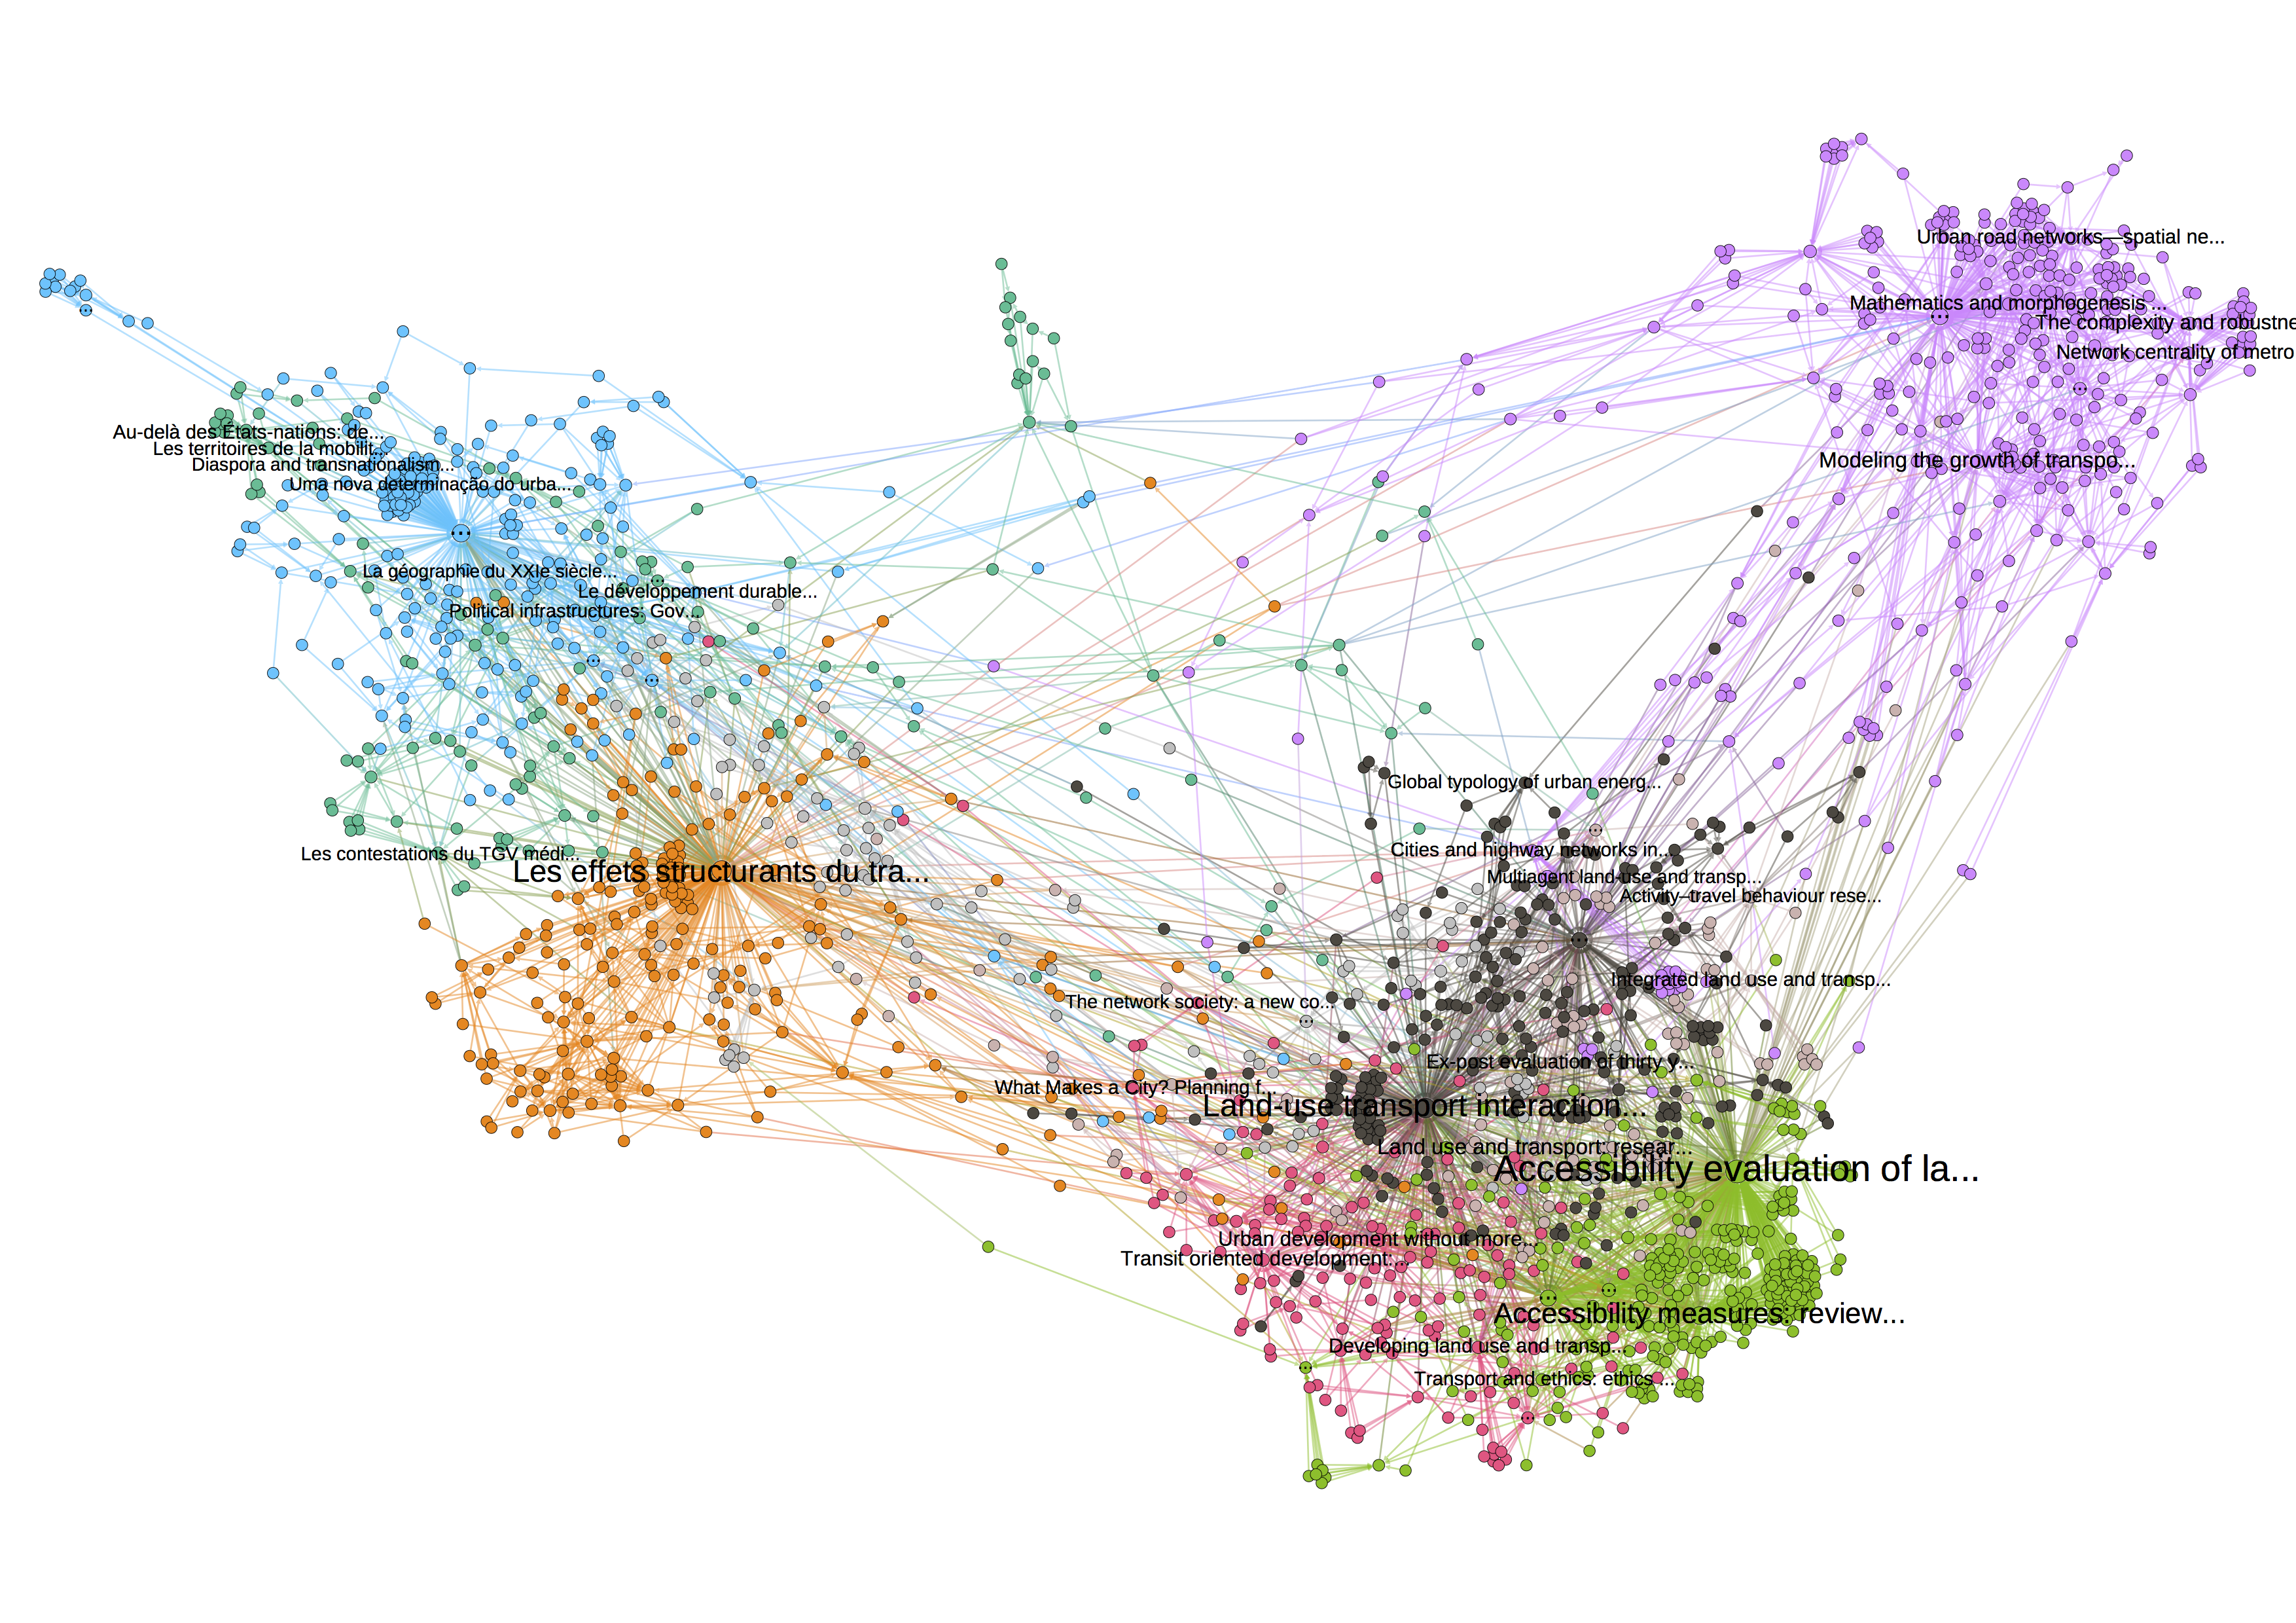
\includegraphics[width=\linewidth]{Figures/QuantEpistemo/rawcore}
\caption[Citation Network][Réseau de citations]{\textbf{Citation Network}\label{fig:quantepistemo:citnw}}{\textbf{Réseau de citations.} Nous visualisons les références ayant au moins deux liens, par un algorithme de force-atlas. Les couleurs donnent les communautés décrites dans le texte. En orange, bleu, turquoise: géographie urbaine, géographie des transports, sciences politiques ; en rose, noir, vert: planning, accessibilité, LUTI ; en violet : réseaux spatiaux (physique et économie).\label{fig:quantepistemo:citnw}}
\end{figure}
%%%%%%%%%%%%%%%%%





%%%%%%%%%%%%%%%%%%
\paragraph{Semantic Communities}{Communautés Sémantiques}


L'extraction des mots-clés est faite suivant une heuristique inspirée de~\cite{chavalarias2013phylomemetic}. La description complète de la méthode et de son implémentation est donnée en Appendice~\ref{app:sec:cybergeo}. Elle se base sur les relations au second ordre entre les entités sémantiques, qui sont des \emph{n-grams}, c'est à dire des mots-clés multiples pouvant avoir une longueur jusqu'à 3. Celles-ci sont estimées via la matrice de co-occurrence, dont les propriétés statistiques fournissent une mesure de déviation à des co-occurrences uniformes, qui est utilisée pour juger la pertinence des mots-clés. Sélectionnant un nombre fixe de mots-clés pertinents $K_W = 10000$, nous pouvons ensuite construire un réseau pondéré par les co-occurrences.


\bpar{
The topology of raw networks does not allow the extraction of clear communities, in particular because of the presence of hubs that correspond to frequent terms common to many fields (e.g. \texttt{model}, \texttt{space}). We assume these highest degree terms do not carry specific information on particular classes and can be thus filtered given a maximal degree threshold $k_{max}$. Similarly, edge with small weight are considered as noise and filtered according to a minimal edge weight threshold $\theta_w$. Keywords are preliminary filtered by a document frequency window $\left[ f_{min},f_{max} \right]$ which is slightly different from network filtering and complementary. A sensitivity analysis of resulting network topology to these parameters is presented in Fig.~\ref{fig:sensitivity}. We choose parameter values that maximize modularity under the constraint of a community number and size distribution of same magnitude as technological classes. This multi-objective optimization does not have a unique solution as objectives are somehow contradictory, and a compromise point must be chosen.
}{
La topologie du réseau brut ne permet pas l'extraction claire de communautés, en particulier à cause de hubs qui correspondent à des termes fréquents commun à de nombreux champs (e.g. \texttt{model}, \texttt{space})\comment[FL]{statut de ces mots ?}. Nous faisons l'hypothèse que ces termes à fort degré ne portent pas d'information particulière sur des classes données et peuvent ainsi être filtrés étant donné un seuil de degré maximal $k_{max}$ (on s'intéresse alors à ce qui fait la spécificité de chaque domaine). De la même manière, les liens avec un poids faibles sont considérés comme du bruit et filtrés selon un seuil de poids minimal $\theta_w$. La méthode générique permet de plus une filtration préliminaire des mot-clés, complémentaire à la filtration topologique, par fréquence d'apparition dans les documents $\left[ f_{min},f_{max} \right]$, à laquelle les résultats ne sont pas sensibles dans notre cas. L'analyse de sensibilité des caractéristiques du réseau filtré, notamment de sa taille, modularité et structure des communautés, est donnée en~\ref{app:sec:quantepistemo}. Nous choisissons des valeurs de paramètres permettant une optimisation multi-objectif entre modularité et taille du réseau, $\theta_w = 10,k_{max} = 500$, par le choix d'un point compromis sur un front de Pareto, qui donne un réseau sémantique de taille $(V=7063,E=48952)$. Celui-ci est visualisé en Appendice~\ref{app:sec:quantepistemo}.
}


\bpar{
We then retrieve communities in the semantic network (using standard Louvain algorithm, with the optimized filtering parameters). communities correspond to well-defined scientific fields (and/or domains, approaches). An expert validation allow us to give names to these, a more complicated naming procedure would eventually be possible (as in~\cite{yang2000improving} for the case of patents 
 where a chi-square test on distribution of documents in classes), but we prefer to stick here to a certain level of supervision. Table~\ref{tab:domains} summarizes the communities 
}{
Nous récupérons ensuite les communautés dans le réseau par un clustering de Louvain standard sur le réseau filtré optimal. On obtient 20 communautés pour une modularité de 0.58. Celles-ci sont examinées à la main pour être nommées, les techniques de désignation automatique~\cite{yang2000improving} n'étant pas assez élaborées et ne font pas la distinction implicite entre champs thématiques et méthodologiques par exemple (en fait entre les domaines de connaissance, voir~\ref{sec:knowledgeframework}) qui est une dimension supplémentaire que nous ne traitons pas ici, mais nécessaire pour avoir des désignations parlantes. Les communautés sont décrites en Table~\ref{tab:quantepistemo:semanticdomains}. On voit tout de suite la complémentarité avec l'approche par citation, puisque se dégagent ici à la fois des sujet d'étude (High Speed Rail, Maritime Networks), des domaines et méthodes (Networks, Remote Sensing, Mobility Data Mining), des domaines thématiques (Policy), des méthodes pures (Agent-based Modeling, Measuring). Ainsi, une référence peut mobiliser plusieurs de ces communautés. On a de plus une granularité plus fine de l'information. L'effet du langage est puissant puisque la géographie française se distingue en une catégorie séparée (des analyses poussées pourraient être envisagées pour mieux comprendre le phénomène et en tirer parti: sous-communautés, reconstruction d'un réseau spécifique, études par traduction ; mais celles-ci sont hors de propos dans cette étude exploratoire). On constante l'importance des réseaux, des problématiques de sciences politiques et socio-économiques. Nous mobiliserons la première catégorie dans la plupart des modèles développés, mais en gardant en tête l'importance des problématiques liées à la gouvernance, nous réaliserons un travail spécifique en~\ref{sec:lutetia}.
}




%%%%%%%%%%%%%%%%%%
\begin{table}
\caption[Semantic communities][Communautés sémantiques]{Disciplines/domains/fields reconstructed from community detection in the semantic network}{\textbf{Description des communautés sémantiques.} On donne leur taille, leur proportion en quantité de mots-clés cumulés sur l'ensemble du corpus, et des mots-clés représentatifs sélectionnés par degré maximal.\comment[FL]{pourquoi ces mots sont ils tronques ?}[(JR) cest explique dans le texte (surtout en annexe) il s'agit de stem]}
\label{tab:quantepistemo:semanticdomains}
\begin{tabular}{llll}
\hline\noalign{\smallskip}
Name & Size & Weight & Keywords  \\
\noalign{\smallskip}\hline\noalign{\smallskip}
Networks & 820 & 13.57\% & \texttt{social network, spatial network, resili} \\
Policy & 700 & 11.8\% & \texttt{actor, decision-mak, societi} \\
Socio-economic & 793 & 11.6\% & \texttt{neighborhood, incom, live} \\
High Speed Rail & 476 & 7.14\% & \texttt{high-spe, corridor, hsr} \\
French Geography & 210 & 6.08\% & \texttt{système, développement, territoire} \\
Education & 374 & 5.43\% & \texttt{school, student, collabor} \\
Climate Change & 411 & 5.42\% & \texttt{mitig, carbon, consumpt} \\
Remote Sensing & 405 & 4.65\% & \texttt{classif, detect, cover} \\
Sustainable Transport & 370 & 4.38\% & \texttt{sustain urban, travel demand, activity-bas} \\
Traffic & 368 & 4.23\% & \texttt{traffic congest, cbd, capit} \\
Maritime Networks & 402 & 4.2\% & \texttt{govern model, seaport, port author} \\
Environment & 289 & 3.79\% & \texttt{ecosystem servic, regul, settlement} \\
Accessibility & 260 & 3.23\% & \texttt{access measur, transport access, urban growth} \\
Agent-based Modeling & 192 & 3.18\% & \texttt{agent-bas, spread, heterogen} \\
Transportation planning & 192 & 3.18\% & \texttt{transport project, option, cba} \\
Mobility Data Mining & 168 & 2.49\% & \texttt{human mobil, movement, mobil phone} \\
Health Geography & 196 & 2.49\% & \texttt{healthcar, inequ, exclus} \\
Freight and Logistics & 239 & 2.06\% & \texttt{freight transport, citi logist, modal} \\
Spanish Geography & 106 & 1.26\% & \texttt{movilidad urbana, criteria, para} \\
Measuring & 166 & 1.0\% & \texttt{score, sampl, metric} \\
\noalign{\smallskip}\hline
\end{tabular}
\end{table}
%%%%%%%%%%%%%%%%%%



%%%%%%%%%%%%%%%%%%
\paragraph{Measures of Interdisciplinarity}{Mesures d'interdisciplinarité}


\bpar{
Distribution of keywords within communities provides an article-level interdisciplinarity.
Combination of citation and semantic layers in the hyper-network provide second order interdisciplinarity measures, that we don't use here because of the modest size of the citation network. More precisely, a reference can be viewed as a probability vector on semantic classes.
}{
La distribution des mots clés dans les communautés permettent de définir une mesure d'interdisciplinarité au niveau de l'article. La combinaison des couches de citation et sémantique dans l'hyperréseau fournit des mesures d'interdisciplinarité au second ordre (motifs sémantiques des cités ou des citants), que nous n'utiliserons pas ici à cause de la taille modeste du réseau de citation (voir \ref{app:sec:cybergeo} et \ref{app:sec:patents}). Plus précisément, une référence $i$ peut être vue comme un vecteur de probabilités sur les classes sémantiques $j$, qu'on notera sous forme matricielle $\mathbf{P}=(p_{ij})$. Celles-ci sont estimées simplement par les proportions de mots-clés classifiés dans chaque classe pour la référence. Une mesure classique d'interdisciplinarité~\cite{bergeaud2017classifying} est alors $I_i = 1 - \sum_j p_{ij}^2$. Soit $\mathbf{A}$ la matrice d'adjacence du réseau de citation, et soit $\mathbf{I}_k$ les matrices de selection des lignes correspondants à la classe $k$ de la classification de citation: $Id\cdot \mathbbm{1}_{c(i)=k}$, telle que $I_k \cdot A \cdot I_{k'}$ donne exactement les citations de $k$ vers $k'$. La proximité de citation entre les communautés de citation est alors définie par $c_{kk'} = \sum \mathbf{I}_k \cdot \mathbf{A} \cdot \mathbf{I}_{k'} /  \sum \mathbf{I}_k \cdot \mathbf{A}$. On définit la proximité sémantique en définissant une matrice de distance entre références par $\mathbf{D} = d_{ii'}=\sqrt{\frac{1}{2}\sum (p_{ij}-p{i'j})^2}$ puis la proximité sémantique par $s_{kk'} = \mathbf{I}_k \cdot \mathbf{D} \cdot \mathbf{I}_{k'} / \sum \mathbf{I}_k \sum \mathbf{I}_{k'}$. Nous montrons en Fig.~\ref{fig:quantepistemo:interdisc} les valeurs de ces différentes mesures, ainsi que la composition sémantique des communautés de citation, pour les classes sémantiques majoritaires. La distribution de $I_i$ montre que les papiers gravitant dans le domaine du LUTI sont les plus interdisciplinaires dans les termes utilisés, ce qui pourrait être lié à leur caractère appliqué. Les autres disciplines sont dans des motifs similaires, à part la géographie et la planification des infrastructures qui présentent des distributions quasi-uniformes, témoignant de l'existence de références très spécialisées dans ces classes. Ce n'est pas nécessairement étonnant vu les sous-champs pointus exhibés (sciences politiques par exemples, et de même les études prospectives type coût-bénéfices sont très étriquées). Ce premier croisement des couches nous confirme les spécificités de chaque champ. Concernant les compositions sémantiques, la plupart agissent comme validation externe vu les classes majoritaires. Le champ le moins concerné par les problème socio-économiques est la planification des infrastructure, ce qui donnera du grain à moudre aux détracteurs de la technocratie. Les questions de changement climatique et durabilité sont relativement bien répartie. Enfin, les ouvrages géographiques concernent en majorité des problèmes de gouvernance. Les matrices de proximité confirment la conclusion de la sous-section précédente en terme de citation, les partages étant très faibles, les plus hautes valeurs étant jusqu'à un quart de la planification vers la géographie et des LUTI vers le TOD (mais pas l'inverse, les relations peuvent être à sens unique). Hors, les proximités sémantiques montrent par exemple que LUTI, TOD, Accessibility et Networks sont proches dans leur termes, ce qui est logique pour les trois premiers, et confirme pour le dernier que les physiciens se basent majoritairement sur les méthodes des ces champs liés au planing pour légitimer leur travaux. La géographie est totalement isolée, sa plus proche voisine étant la planification des infrastructures. Cette étude est très utile pour notre propos, puisqu'elle montre des domaines cloisonnés partageant des termes at donc a priori des problématiques et sujet commun. On ne se parle pas alors qu'on parle des languages pas si lointains, d'où la pertinence accrue de les faire parler d'une commune voie dans nos travaux : nos modèles devront mobiliser des éléments, ontologies et échelles de ces différents champs.
}



%%%%%%%%%%%%%%%%%%
\begin{figure}
\includegraphics[width=0.49\linewidth]{Figures/QuantEpistemo/interdisciplinarities}
\includegraphics[width=0.49\linewidth]{Figures/QuantEpistemo/compo_proportion}\\
\includegraphics[width=0.49\linewidth]{Figures/QuantEpistemo/citation_proximities}
\includegraphics[width=0.49\linewidth]{Figures/QuantEpistemo/semantic_proximities}
\caption[][Motifs d'interdisciplinarité]{\label{fig:quantepistemo:interdisc}}{\textbf{Motifs d'interdisciplinarité.} \textit{(Haut Gauche)} Distribution des $I_i$ par classes de citations ; \textit{(Haut Droite)} Composition sémantiques des classes de citation ; \textit{(Bas Gauche)} Matrice de proximité de citation $c_{kk'}$ entre classes de citations ; \textit{(Bas Droite)} Matrice de proximité sémantique $s_{kk'}$ entre classes de citations.\label{fig:quantepistemo:interdisc}\comment[FL]{tu compares les disciplines entre elles mais pas la facon dont elles attaquent les questions au coeur de ta these. c'est dommage.}[(JR)c'est l'objet de la section suivante]}
\end{figure}
%%%%%%%%%%%%%%%%%%



% bootstrap
%min(corrs);max(corrs);mean(abs(corrs))
% -0.170952  0.5496791  0.08384802
% apply(bcorrs,2,mean)
%       minrho        maxrho    meanabsrho     minrhosup     maxrhosup meanabsrhosup 
%  -0.08792137    0.11690677    0.03137750   -0.17686637    0.68579406    0.11079253 
% apply(bcorrs,2,sd)
%       minrho        maxrho    meanabsrho     minrhosup     maxrhosup meanabsrhosup 
%  0.012683338   0.021324056   0.002250636   0.038402781   0.134996447   0.051553244 

% modularities
% sem : 0.1053156
% cit : 0.8140818
% bootstrap N=100
% sem : 0.073097051446193 +- 0.00307154703966512
% cit : 0.204223565075042 +- 0.0141450119581389


\bpar{
}{
Nous concluons cette analyse par une approche plus robuste pour quantifier les proximités entre couches de l'hyperréseau. Il est aisé de construire une matrice de corrélation entre deux classifications, par les corrélations de leur colonnes. Nous définissons les probabilités $\mathbf{P}_C$ toutes égales à 1 pour la classification de citation. La matrice de correlation de celle-ci avec $\mathbf{P}$ s'étend de -0.17 à 0.54 et a une moyenne de valeur absolue de 0.08, ce qui est significatif par rapport à des classifications aléatoire puisque un bootstrap à $b=100$ répétitions avec les matrices mélangées donne un minimum à $-0.08 \pm 0.012$, un maximum à $0.11 \pm 0.02$ et une moyenne absolue à $0.03 \pm 0.002$. Cela montre que les classifications sont complémentaires et que cette complémentarité est significative statistiquement par rapport à des classifications aléatoires. L'adéquation de la classification sémantique par rapport au réseau de citation peut également être quantifiée par la modularité multi-classes~\cite{nicosia2009extending} (voir~\ref{sec:app:patents} pour une définition mathématique), qui traduit la probabilité qu'un lien soit dû à la classification étudiée, en prenant en compte l'appartenance simultanée à de multiples classes. Ainsi, la modularité multi-classes des probabilités sémantiques pour le réseau de citation est de 0.10, ce qui d'une part est significativement signe d'adéquation, un bootstrap toujours à $b=100$ donnant une valeur de $0.073 \pm 0.003$, qui reste limitée vu la valeur maximale fixée par les probabilités de citations dans leur propre réseau qui donnent une valeur de 0.81, ce qui confirme d'autre part la complémentarité des classifications.
}








%--------------------------------------------------------------



%%%%%%%%%%%%%%%%%%%%%%%%
\subsection{Discussion}{Discussion}




\subsubsection{Towards modeling purpose and context automatic extraction}{Vers une modélisation des thèmes et une extraction automatique du contexte}


\bpar{
A possible direction to strengthen our quantitative epistemological analysis would be to work on full textes related to the modeling of interaction between networks and territories, with the aim to automatically extract thematics within articles. The idea would be to perform some kind of automatized modelography, with possible features to be extracted that would be ontologies, model architecture or structures, scales, or even typical parameter values. It is not clear to what degree structure of models can be extracted from their description in papers and it surely depends on the discipline considered. For example in a framed field such as transportation planning, using a pre-defined ontology (in the sense of dictionary) and a fuzzy grammar could be efficient to extract information as the discipline is relatively formatted. In theoretical and quantitative geography, beyond the barrier of language, information organisation is surely less subject to unsupervised data-mining because of the more literary nature of the discipline : synonyms and figures of speech are generally the norm in good level human sciences writing, fuzzing a possible generic structure of knowledge description. 
}{
Une direction possible pour renforcer cette analyse en épistémologie quantitative serait de travailler sur les textes complets des références contenant des efforts de modélisations des interactions entre réseaux et territoires, avec le but d'extraire automatiquement les thématiques des articles. Des méthodes plus adaptées pour les long texte que celle utilisée ici incluent par exemple l'Allocation Latente de Dirichlet~\cite{blei2003latent}. L'idée serait de procéder à une sorte de modélographie automatique, pour extraire des caractéristiques telle les ontologies, l'architecture ou la structure des modèles, les échelles ou même des valeurs typiques des paramètres. Il n'est pas clair dans quelle mesure la structure des modèles peut être extraite de leur description dans un article, et cela dépend sûrement de la discipline considérée. Par exemple dans champ relativement cadré comme la planification des transports, l'utilisation d'une ontologie pré-définie (dans le sens d'un dictionnaire) et d'une grammaire floue pourrait être efficace vu les conventions assez strictes dans la discipline. En géographie théorique et quantitative, au delà de la barrière du language\comment[FL]{?}, l'organisation de l'information est sûrement plus délicate à appréhender par de l'apprentissage non-supervisé à cause de la nature plus littéraire de la discipline : les synonymes et les figures de style sont généralement la norme pour l'écriture d'un bon niveau en sciences humaines, rendant plus floue une possible structure générique de la description des connaissances.
}


%Depending on extended results of the two previous sections and on thematic requirements (huge need of knowledge on precise models structure, that may appear when trying to construct more specialized operational models), this project may be conducted with more or less investment.




\subsubsection{Reflexivity}{Réflexivité}


\bpar{
The methodology developed here is particularly interesting since it is reflexive, i.e. it can be used on our work itself. Therefore, an other application will be the reflexivity of our thesis : we attend to proceed to similar analysis on our proper bibliography (and possibly its evolution, available via \texttt{git} history), to understand our patterns of knowledge, possible gaps or unveil unexpected developments. The detailed development is done in Appendix~\ref{app:reflexivity}.
}{
La méthodologie que nous avons développé ici est particulièrement intéressante puisqu'elle offre des potentialités de réflexivité, c'est à dire qu'elle peut être utilisée pour étudier notre approche elle-même. Une de ses applications, hors de celle à la revue scientifique Cybergeo dans la perspective de Science Ouverte (voir Appendice~\ref{app:sec:cybergeo}), sera à notre propre corpus de références, dans le but de révéler des possibles  directions de recherche ou problématiques exotiques. Il est éventuellement possible de le faire de manière dynamique, grâce à l'historique de \texttt{git} qui permet de récupérer n'importe quelle version de la bibliographie à une date donnée sur les trois ans écoulés. Il s'agira aussi de comprendre nos motifs de production de connaissance afin de contribuer à~\ref{sec:knowledgeframework}. Le développement détaillé est fait en Appendice~\ref{app:reflexivity}.
}





\stars




%%%%%%%%%%%%%%%%%%%%%%%%%%%%%




%%%%%%%%%%%%%%%%%%%%%%%%%%%%%
% Chapter : Quantitative Epistemology



% Chapter 

\chapter{Methodological Developments} % Chapter title

\label{ch:methodology} % For referencing the chapter elsewhere, use \autoref{ch:name} 

%----------------------------------------------------------------------------------------

\headercit{We are now building a rigorous Science of Cities, contrarily to what was done before.}{Marc Barth{\'e}l{\'e}my}{}

\bigskip

Such a shocking phrase was pronounced during the introduction of a \emph{Network} course for students of Complex System Science. Besides the fact that the spirit of CSS is precisely the opposite, {\ie} the construction of integrative disciplines (vertical integration that is necessarily founded on the existing body of knowledge of concerned fields) that answer transversal questions (horizontal integration that imply interdisciplinarity) - see {\eg} the roadmap for CS~\cite{2009arXiv0907.2221B}, it reveals how methodological considerations shape the perceptions of disciplines. From a background in Physics, ``rigorous'' implies the use of tools and methods judged more rigorous (analytical derivations, large datasets statistics, etc.). But what is rigorous for someone will not be for an other discipline\footnote{a funny but sad anecdote told by a friend comes to mind : defending his PhD in statistics, he was told at the end by economists how they were impressed by the mathematical rigor of his work, whereas a mathematician judged that ``he could have done everything on the back of an enveloppe''.}, depending on the purpose of each piece of research (perspectivism~\cite{giere2010scientific} poses the \emph{model}, that includes methods, as the articulating core of research entreprises). Thus the full role of methodology aside and not beside theory and experiments. We go in this chapter into various methodological developments which may be precisely used later or contribute to the global background.

We first propose a kind of essay insisting on the importance of reproducibility in science. More than a guideline, it is a way to practice science that a necessary condition for its rigor. Any non-reproducible work is not scientific. We then derive technical results on models of urban growth and on the sensitivity of scaling laws, that are both recurrent themes in the modeling of complex urban systems. We then introduce a method in the context of systematic model exploration and model behavior. We finally work on a link between static and dynamic correlations in a geographical system. This chapter is rather heteroclite as sections may correspond to a particular technical need at a point in the thesis, to global methodological directions, or global research directions.



%----------------------------------------------------------------------------------------

\newpage

% Section : Reproducibility


\section{Reproducibility}




The strength of science comes from the cumulative and collective nature of research, as progresses are made as Newton said ``standing on the shoulder of giants'', meaning that the scientific enterprise at a given time relies on all the work done before and that advances would not be possible without constructing on it. It includes development of new theories, but also extension, testing or falsifiability of previous ones. In that context 





As scientific reproducibility is an essential requirement for any study, its practice seems to be increasing~\cite{stodden2010scientific} and technical means to achieve it are always more developed (as e.g. ways to make data openly available, or to be transparent on the research process such as \texttt{git}~\cite{ram2013git}, or to integrate document creation and data analysis such as \texttt{knitr}~\cite{xie2013knitr}), at least in the field of numerical modeling and simulation. However, the devil is indeed in the details and obstacles judged at first sight as minor become rapidly a burden for reproducing and using results obtained in some previous researches. We describe two cases studies where models of simulation are apparently highly reproducible but unveil as puzzles on which research-time balance is significantly under zero, in the sense that trying to exploit their results may cost more time than developing from scratch similar models.






%%%%%%%%%%%%%%%%%%%%%%%%%%%%%%%%%%
\subsection{On the Need to Explicit the Model}

A current myth is that providing entire source code and data will be a sufficient condition for reproducibility. It will work if the objective is to produce exactly same plots or statistical analysis, assuming that code provided is the one which was indeed used to produce the given results. It is however not the nature of reproducibility. First, results must be as much implementation-independent as possible for clear robustness purposes. Then, in relation with the precedent point, one of the purposes of reproducibility is the reuse of methods or results as basis or modules for further research (what includes implementation in another language or adaptation of the method), in the sense that reproducibility is not replicability as it must be adaptable~\cite{drummond2009replicability}.

Our first case study fits exactly that scheme, as it was undoubtedly aimed to be shared with and used by the community since it is a model of simulation provided with the Agent-Based simulation platform NetLogo~\cite{wilensky1999netlogo}. The model is also available online~\cite{de2007netlogo} and is presented as a tool to simulate socio-economic dynamics of low-income residents in a city based on a synthetic urban environment, generated to be close in stylized facts from the real town of Tijuana, Mexico. Beside providing the source code, the model appears to be poorly documented in the literature or in comments and description of the implementation. Comments made thereafter are based on the study of the urban morphogenesis part of the model (setup for the ``residential dynamics'' component) as it is our global context of study~\cite{raimbault2014vers}. In the frame of that study, source code was modified and commented, which last version is available on the repository of the project\footnote{at \texttt{https://github.com/JusteRaimbault/CityNetwork/tree/master/Models/Reproduction/UrbanSuite}}.




\paragraph{Rigorous Formalization}

An obvious part of model construction is its rigorous formalization in a formal framework distinct from source code. There is of course no universal language to formulate it~\cite{banos2013pour}, and many possibilities are offered by various fields (e.g. UML, DEVS, pure mathematical formulation). No paper nor documentation is provided with the model, apart from the embedded NetLogo documentation since it only thematically describes in natural language the ideas behind each step without developing more and provides information about role of different elements of the interface.

This formulation is a key for it to be understood, reproduced and adapted ; but it also avoids implementation biases such as
\begin{itemize}
\item Architecturally dangerous elements : in the model, world context is a torus and agents may ``jump'' in the euclidian representation, what is not acceptable for a 2D projection of real world. To avoid that, many tricky tests and functions were used, including unadvised practices (e.g. dead of agents based on position to avoid them jumping).
\item Lack of internal consistence : the example of the patch variable \texttt{land-value} used to represent different geographical quantities at different steps of the model (morphogenesis and residential dynamics), what becomes an internal inconsistence when both steps are coupled when option \texttt{city-growth?} is activated.
\item Coding errors : in an untyped language such as NetLogo, mixing types may conduct to unexpected runtime errors, what is the case of the patch variable \texttt{transport} in the model (although no error occurs in most of run configurations from the interface, what is more dangerous as the developer thinks implementation is secure). Such problems should be avoided if implementation is done from an exact formal description of the model.
\end{itemize}


\paragraph{Transparent Implementation}

A totally transparent implementation is expected, including ergonomics in architecture and coding, but 

\paragraph{Expected Model Behavior}

Whatever the definition, a model can not be reduced to its formulation and/or implementation, as expected model behavior or model usage can be viewed as being part of the model itself. In the frame of \noun{Giere}'s perspectivism~\cite{giere2010scientific}, the definition of model includes the purpose of use but also the agent who aims to use it. Therefore a minimal explication of model behavior and exploration of parameter roles is highly advised to decrease chances of misuses or misinterpretations of it. It includes simple runtime charts that are immediate on the NetLogo platform, but also indicators computations to evaluate outputs of the model. It can also be improved visualizations during runtime and model exploration, such as showed in Fig.~\ref{fig:example_tij_viz}.

\begin{figure}
\centering

\hspace{-2cm}
\includegraphics[width=0.33\textwidth]{Figures/PartI/Methodology/Reproducibility/stdView}
\hfill
\includegraphics[width=0.33\textwidth]{Figures/PartI/Methodology/Reproducibility/ViewRoads}
\hfill
\includegraphics[width=0.33\textwidth]{Figures/PartI/Methodology/Reproducibility/landValues_cityFinished}
\caption[Reproducibility and visualization]{Example of simple improvement in visualization that can help understanding mechanisms implied in the model. \textit{Left : } example of original output ; \textit{Middle : } visualization of main roads (in red) and underlying patches attribution, suggesting possible implementation bias in the use of discretized trace of roads to track their positions ; \textit{Right : }Visualization of land values using a more readable color gradient. This step confirms the hypothesis, through the form of value distribution, that the morphogenesis step is an unnecessary detour to generate a random field for which simple diffusion method should provide similar results, as detailed in the paragraph on implementation.}
\label{fig:example_tij_viz}
\end{figure}




\subsection{On the Need of Exactitude in Model Implementation}

% Barthelemy paper, pb in model description/implementation
%  - test different analyses with possible biaises -

Possible divergences between model description in a paper and the effectively implemented processes may have grave consequences on the reproducibility of science. The road network growth model given in~\cite{barthelemy2008modeling} is one example that we are currently investigating. A strict implementation of model mechanisms provide slightly different results than the one presented in the paper, and as source code is not provided we need to test different hypotheses on possible mechanisms added by the programmer (that seems to be a connexion rule to intersections under a certain distance threshold). Lessons that could be possibly drawn from this examples are 
\begin{itemize}
\item the necessity of providing source code
\item the necessity of providing architecture description along with code (if model description is in a langage too far from architectural specifications) in order to identify possible implementation biaises
\item the necessity of performing and detailing explicitly model explorations, that would in that case have helped to identify the implementation bias.
\end{itemize}

The last point, if first not provided, may ensure a limited risk of scientific falsification as it may be more complicated to fake false exploration results than to effectively explore the model. A joint project currently done is the writing of a false modeling paper in the spirit of~\cite{zilsel2015canular}, in which opposite results to the effective results of a given model are provided, without providing model implementation. A first bunch of test is the acceptance of a clearly non-reproducible paper in diverse journals, possibly with a control on textual elements (using or not ``buzz-words'' associated to the journal, etc.). Depending on results, a second experiment may be tested with providing open source code for model implementation but still with false results, to verify if reviewers effectively try to reproduce results when they pretend to want the code (in reasonable computational power limits of course, HPC being not currently broadly available in Humanities).



\subsection{Perspectives}


Again, reproducibility and transparency is a non-negotiable feature of contemporaneous science, along with Open practices and Open Access. Too much examples (see a very recent one in experimental economics~\cite{camerer2016evaluating}) show in various disciplines the lack of reproducibility of experiments, that is a falsification of previous results or a result in itself. Falsification is a costly practice, and even if necessary~\cite{chavalarias2005nobel}, could be made more efficient through more transparency and direct reproducibility, increase therein the global workflow of science. We develop in parallel of this thesis various tools aimed to ease reproducibility, for which an overview is given in appendix~\ref{app:workflow}.



%----------------------------------------------------------------------------------------

% Section : stochastic framework for urban growth


\newpage

\section{An unified framework for stochastic models of urban growth}

Urban growth modeling fall in the case of tentatives to find self-consistent rules reproducing dynamics of an urban system, and thus in our logic of system morphogenesis. We examine here methodological issues linked to different frameworks of urban growth.

%%%%%%%%%%%%%%%%%%%%
\subsection{Introduction}
%%%%%%%%%%%%%%%%%%%%

Various stochastic models aiming to reproduce population patterns on large temporal and spatial scales (city systems) have been discussed across various fields of the literature, from economics to geography, including models proposed by physicists. We propose here a general framework that allows to include different famous models (in particular Gibrat, Simon and Preferential Attachment model) within an unified vision. It brings first an insight into epistemological debates on the relevance of models. Furthermore, bridges between models lead to the possible transfer of analytical results to some models that are not directly tractable.


%%%%%%%%%%%%%%%%%%%%
%\subsubsection{Context}

Seminal models of urban growth are Simon~\cite{simon1955class} (later generalized as e.g. \cite{haran1973modified}) and Gibrat models. Many examples can be given across disciplines. \cite{benguigui2007dynamic} give an equation-based dynamical model, whereas \cite{gabaix1999zipf} solves a stationary model. \cite{Gabaix20042341} reviews urban growth approaches in economics. A model adapted from evolutive urban theory is solved in~\cite{favaro2011gibrat} and improves Gibrat models. The question of empirical scales at which it is consistent to study urban growth was also tackled in the particular case of France~\cite{bretagnolle2002time}. We stay to a certain level of tractability to include models as essence of our approach is links between models but do not make ontologic assumptions.


%%%%%%%%%%%%%%%%%%%%
%\subsubsection{Notations}



%%%%%%%%%%%%%%%%%%%%
\subsection{Framework}
%%%%%%%%%%%%%%%%%%%%


%%%%%%%%%%%%%%%%%%%%
%\subsubsection{Formulation}

\paragraph{Presentation}
What we propose as a framework can be understood as a meta-model in the sense of~\cite{cottineau2015incremental}, i.e. an modular general modeling process within each model can be understood as a limit case or as a specific case of another model. More simply it should be a diagram of formal relations between models. The ontological aspect is also tackled by embedding the diagram into an ontological state space (which discretization corresponds to the ``bricks'' of the incremental construction of~\cite{cottineau2015incremental}). It constructs a sort of model classification or modelography.

We are still at the stage of different derivations of links between models that are presented hereafter.

%\subsubsection{Models Included}

%The following models are included in our framework. The list is arbitrary but aims to offer a broad view of disciplines concerned

%\subsubsection{Thematic Classification}


%\subsubsection{Framework Formulation}
%Diagram linking various models ; first embedded into time/population plane, cases Discrete/Continous. Other aspects more sparse (ex. spatialization) ; how represent it ?

%%%%%%%%%%%%%%%%%%%%
%\subsection{Models formulation}



%%%%%%%%%%%%%%%%%%%%
\subsection{Derivations}

\subsubsection{Generalization of Preferential Attachment}

\cite{yamasaki2006preferential} give a generalization of the classical Preferential Attachment Network Growth model, as a birth and death model with evolving entities. More precisely, network units gain and lose population (equivalent to links connexions) at fixed probabilities, and new unit can be created at a fixed rate.

\subsubsection{Link between Gibrat and Preferential Attachment Models}


\bpar{
Let consider a strictly positive growth Gibrat model given by $P_i(t)=R_i(t)\cdot P_{i}(t-1)$ with $R_i(t)>1$, $\mu_i(t)=\Eb{R_i(t)}$ and $\sigma_i(t)=\Eb{R_i(t)^2}$. On the other hand, we take a simple preferential attachment, with fixed attachment probability $\lambda \in [0,1]$ and new arrivants number $m>0$. We derive that Gibrat model can be statistically equivalent to a limit of the preferential attachment model, assuming that the moment-generating function of $R_i(t)$ exists. Classical distributions that could be used in that case, e.g. log-normal distribution, are entirely defined by two first moments, making this assumption reasonable.
}{
Considérons un modèle de croissance strictement positive de Gibrat donnée par $P_i(t)=R_i(t)\cdot P_{i}(t-1)$ avec $R_i(t)>1$, $\mu_i(t)=\Eb{R_i(t)}$ et $\sigma_i(t)=\Eb{R_i(t)^2}$. D'autre part, soit un modèle simple d'attachement préférentiel, avec une probabilité d'attachement $\lambda \in [0,1]$ et un nombre de nouveau arrivants $m>0$. Il est possible de dériver que le Gibrat est statistiquement équivalent à une limite de l'attachement préférentiel, sous l'hypothèse que toutes les fonctions génératrices des moments de $R_i(t)$ existent. Les distributions classiques qui peuvent être utilisées dans ce cas, e.g. une distribution normale ou log-normale, sont entièrement déterminées par leur deux premiers moments, ce qui rend cette hypothèse raisonnable.
}



\begin{lemma}
The limit of a Preferential Attachment model when $\lambda \ll 1$ is a linear-growth Gibrat model, with limit parameters $\mu_i(t)=1+\frac{\lambda}{m\cdot (t-1)}$.
\end{lemma}


\bpar{
The proof is given in Appendix~\ref{app:technical}.
}{
La preuve est donnée en Annexe~\ref{app:technical}.
}


\subsubsection{Link between Simon and Preferential Attachment}
%\label{subsubsec:gibrat-simon}

A rewriting of Simon model yields a particular case of the generalized preferential attachment, in particular by vanishing death probability.

\subsubsection{Link between Favaro-Pumain and Gibrat}

\cite{favaro2011gibrat} generalizes Gibrat models with innovation propagation dynamics, being therefore a generalization of that model. Theoretically, a process-based model equivalent to the Favaro-pumain should then fill the missing case in model classification at the corresponding discretization. Simpop models do not fill that case as they stay at the scale of city systems, as for Marius models~\cite{cottineau2014evolution}. These must also have their counterparts in discrete microscopic formulation.

\subsubsection{Link between Bettencourt-West and Pumain}

We are considering to study Bettencourt-West model for urban scaling laws \cite{bettencourt2008large} as entering the stochastic urban growth framework as stationary component of a random growth model, but investigation are still ongoing.


\subsubsection{Other Models}

\cite{gabaix1999zipf} develops an economic model giving a Simon equivalent formulation. They in particular find out that in upper tail, proportional growth process occurs. We find the same result as a consequence of the derivation of the link between Gibrat and Preferential attachment models.




%%%%%%%%%%%%%%%%%%%%
%\subsection{Application and Perspectives}
%%%%%%%%%%%%%%%%%%%%







%%%%%%%%%%%%%%%%%%%%
%\subsection{Discussion}
%%%%%%%%%%%%%%%%%%%%

%%%%%%%%%%%%%%%%%%%%
%\subsection*{Conclusion}
%%%%%%%%%%%%%%%%%%%%





%----------------------------------------------------------------------------------------

\newpage


%  section : scaling sensitivity : useful ?


\section{Analytical Sensitivity of Urban Scaling Laws to Spatial Extent}

At the center of evolutive urban theory are hierarchy and associated scaling laws. We begin here an methodological investigation on the sensitivity of scaling laws to city definition.


%%%%%%%%%%%%%%%%%%%%
\subsection{Introduction}



Scaling laws have been shown to be universal of urban systems at many scales and for many indicators. Recent studies question however the consistence of scaling exponents determination, as their value can vary significantly depending on thresholds used to define urban entities on which quantities are integrated, even crossing the qualitative border of linear scaling, from infra-linear to supra-linear scaling. We use a simple theoretical model of spatial distribution of densities and urban functions to show analytically that such behavior can be derived as a consequence of the type of spatial distribution and the method used. Numerical simulation confirm the theoretical results and reveals that results are reasonably independent of spatial kernel used to distribute density.



Scaling laws for urban systems, starting from the well-known rank-size Zipf's law for city size distribution~\cite{gabaix1999zipf}, have been shown to be a recurrent feature of urban systems, at many scales and for many types of indicators. They reside in the empirical constatation that indicators computed on elements of an urban system, that can be cities for system of cities, but also smaller entities at a smaller scale, do fit relatively well a power-law distribution as a function of entity size, i.e. that for entity $i$ with population $P_i$, we have for an integrated quantity $A_i$, the relation $A_i \simeq A_0\cdot \left(\frac{P_i}{P_0}\right)^{\alpha}$. Scaling exponent $\alpha$ can be smaller or greater than 1, leading to infra- or supra-linear effects. Various thematic interpretation of this phenomena have been proposed, typically under the form of processes analysis. The economic literature has produced abundant work on the subject (see~\cite{Gabaix20042341} for a review), but that are generally weakly spatial, thus of poor interest to our approach that deals precisely with spatial organization. Simple economic rules such as energetic equilibria can lead to simple power-laws~\cite{bettencourt2008large} but are difficult to fit empirically. A interesting proposition by Pumain is that they are intrinsically due to the evolutionary character of city systems, where complex emergent interaction between cities generate such global distributions~\cite{pumain2006evolutionary}. Although a tempting parallel can be done with self-organizing biological systems, Pumain insists on the fact that the ergodicity assumption for such systems is not reasonable in the case of geographical systems and that the analogy cannot be exploited~\cite{pumain2012urban}. Other explanations have been proposed at other scales, such as the urban growth model at the mesoscopic scale (city scale) given in~\cite{2014arXiv1401.8200L} that shows that the congestion within transportation networks may be one reason for city shapes and corresponding scaling laws. Note that ``classic'' urban growth models such as Gibrat's model do provide first order approximation of scaling systems, but that interactions between agents have to be incorporated into the model to obtain better fit on real data, such as the Favaro-Pumain model for innovation cycles propagation proposed in~\cite{favaro2011gibrat}, that generalize a Gibrat model and provide better fits on data for French cities.

However, the blind application of scaling exponents computations was recently pointed as misleading in most cases~\cite{louf2014scaling}, confirmed by empirical works such as~\cite{2013arXiv1301.1674A} that showed the variability of computed exponents to the parameters defining urban areas, such as density thresholds. An ongoing work by Cottineau \& \textit{al.} presented at~\cite{cottineau2015scaling}, studies empirically for French Cities the influence of 3 parameters playing a role in city definition, that are a density threshold $\theta$ to delimitate boundaries of an urban area, a number of commuters threshold $\theta_c$ that is the proportion of commuters going to core area over which the unity is considered belonging to the area, and a cut-off parameter $P_c$ under which entities are not taken into account for the linear regression providing the scaling exponent. Remarquable results are that exponents can significantly vary and move from infra-linear to supra-linear when threshold varies. A systematic exploration of parameter space produces phase diagrams of exponents for various quantities. One question raising immediately is how these variation can be explained by the features of spatial distribution of variables. Do they result from intrinsic mechanisms present in the system or can they be explained more simply by the fact that the system is particularly spatialized ? We prove on a toy analytical model that even simple distributions can lead to such significant variations in the exponents, along one dimension of parameters (density threshold), directing the response towards the second explanation.
%The rest of the section is organized as follows : we formalize the simple framework used and derive an analytical relation between estimated exponent and density threshold parameter. We then present a numerical implementation of the model that confirms numerically theoretical results, explore other form of kernels that would be less tractable, and study the sensitivity along two parameters. We finally discuss the implications of our results and further work needed.

%%%%%%%%%%%%%%%%%%%%
\subsection{Formalization}
\label{sec:formalization}

We formalize the simple theoretical context in which we will derive the sensitivity of scaling to city definition. Let consider a polycentric city system, which spatial density distributions can be reasonably constructed as the superposition of monocentric fast-decreasing spatial kernels, such as an exponential mixture model~\cite{anas1998urban}. Taking a geographical space as $\mathbb{R}^2$, we take for any $\vec{x}\in\mathbb{R}^2$ the density of population as
\begin{equation}
d(\vec{x}) = \sum_{i=1}^{N}{d_i(\vec{x})} = \sum_{i=1}^{N}{d_i^0\cdot \exp{\left(\frac{-\norm{\vec{x}-\vec{x}_i}}{r_i}\right)}}
\end{equation}

where $r_i$ are spread parameters of kernels, $d_i^0$ densities at origins, $\vec{x}_i$ positions of centers. We furthermore assume the following constraints :

\begin{enumerate}
\item To simplify, cities are monocentric, in the sense that for all $i\neq j$, we have $\norm{\vec{x}_i - \vec{x}_j}\gg r_i$.
\item It allows to impose structural scaling in the urban system by the simple constraint on city populations $P_i$. One can compute by integration that $P_i=2\pi d_i^0 r_i^2$, what gives by injection into the scaling hypothesis $\ln{P_i}=\ln{P_{max}}-\alpha \ln{i}$, the following relation between parameters : $\ln{\left[d_i^0 r_i^2\right]}=K' - \alpha \ln{i}$.
\end{enumerate}

To study scaling relations, we consider a random scalar spatial variable $a(\vec{x})$ representing one aspect of the city, that can be everything but has the dimension of a spatial density, such that the indicator $A(D)=\Eb{\iint_D{a(\vec{x})d\vec{x}}}$ represents the expected quantity of $a$ in area $D$. We make the assumption that $a\in \{0;1\}$ (``counting'' indicator) and that its law is given by $\Pb{a(\vec{x})=1}=f(d(\vec{x}))$. Following the empirical work done in~\cite{cottineau2015scaling}, the integrated indicator on city $i$ as a function of $\theta$ is given by
\[
A_i(\theta) = A(D(\vec{x}_i, \theta))
\]

where $D(\vec{x}_i, \theta)$ is the area centered in $\vec{x}_i$ where $d(\vec{x})>\theta$. Assumption 1 ensures that the area are roughly disjoint circles. We take furthermore a simple amenity such that it follows a local scaling law in the sense that $f(d)=\lambda\cdot d^\beta$. It seems a reasonable assumption since it was shown that many urban variable follow a fractal behavior at the intra-urban scale~\cite{keersmaecker2003using} and that it implies necessarily a power-law distribution~\cite{chen2010characterizing}. We make the additional assumption that $r_i=r_0$ does not depend on $i$, what is reasonable if the urban system is considered from a large scale. This assumption should be relaxed in numerical simulations. The estimated scaling exponent $\alpha(\theta)$ is then the result of the log-regression of $(A_i(\theta))_i$ against $(P_i(\theta))_i$ where $P_i(\theta)=\iint_{D(\vec{x}_i,\theta)}{d}$.


%%%%%%%%%%%%%%%%%%%%
\subsection{Analytical Derivation of Sensitivity}

With above notations, let derive the expression of estimated exponent for quantity $a$ as a function of density threshold parameter $\theta$. The quantity computed for a given city $i$ is, thanks to the monocentric assumption and in a spatial range and a range for $\theta$ such that $\theta \gg \sum_{j\neq i}{d_j(\vec{x})}$, allowing to approximate $d(\vec{x})\simeq d_i(\vec{x})$ on $D(\vec{x}_i,\theta)$, is computed by
\[
\begin{split}
A_i(\theta) & = \lambda\cdot \iint_{D(\vec{x}_i,\theta)}{d^\beta} = 2\pi\lambda {d_i^0}^{\beta} \int_{r=0}^{r_0 \ln{\frac{d_i^0}{\theta}}}{r\exp{\left(-\frac{r\beta}{r_0}\right)}dr}\\
& = \frac{2\pi {d_i^0}^\beta r_0^2}{\beta^2} \left[1 + \beta \ln{\frac{\theta}{d_i^0}\left(\frac{\theta}{d_i^0}\right)^\beta} - \left(\frac{\theta}{d_i^0}\right)^\beta\right]
\end{split}
\]

We obtain in a similar way the expression of $P_i(\theta)$
\[
P_i(\theta) = 2\pi d_i^0 r_0^2 \left[1 + \ln{\left[\frac{\theta}{d_i^0}\right]}\frac{\theta}{d_i^0} - \frac{\theta}{d_i^0}\right]
\]

The Ordinary-Least-Square estimation, solving the problem $\inf_{\alpha,C}\norm{(\ln{A_i(\theta)} - C - \alpha \ln{P_i(\theta)})_i}^2$, gives the value $\alpha(\theta) = \frac{\Covb{(\ln{A_i(\theta)})_i}{(\ln{P_i(\theta)})_i}}{\Varb{(\ln{P_i(\theta)})_i}}$. As we work on city boundaries, threshold is expected to be significantly smaller than center density, i.e. $\theta / d_i^0 \ll 1$. We can develop the expression in the first order of $\theta / d_i^0$ and use the global scaling law for city sizes, what gives $\ln{A_i(\theta)} \simeq K_A - \alpha \ln{i} + (\beta - 1)\ln{d_i^0} + \beta \ln{\frac{\theta}{d_i^0}\left(\frac{\theta}{d_i^0}\right)^\beta} $ and $\ln{P_i(\theta)} = K_P - \alpha \ln{i} + \ln{\left[\frac{\theta}{d_i^0}\right]}\frac{\theta}{d_i^0}$. Developing the covariance and variance gives finally an expression of the scaling exponent as a function of $\theta$, where $k_j,{k_j}'$ are constants obtained in the development :

\begin{equation}
\label{eq:th}
\alpha(\theta) = \frac{k_0 + k_1 \theta + k_2 \theta^\beta + k_3 \theta^{\beta + 1} +  k_4 \theta \ln{\theta} + k_5 \theta^\beta \ln{\theta} + k_6 \theta^\beta (\ln{\theta})^2 + k_7 \theta^{\beta + 1}(\ln{\theta})^2 + k_8 \theta^{\beta + 1}\ln{\theta}}{k_0'+k_1' \ln{\theta} + k_2' \theta \ln{\theta} + k_3' \theta^2 + k_4' \theta^2\ln{\theta} + k_5' \theta^2 (\ln{\theta})^2}
\end{equation}

This rational fraction predicts the evolution of the scaling exponent when the threshold varies. We study numerically its behavior in the next section, among other numerical experiments.


%%%%%%%%%%%%%%%%%%%%
\subsection{Numerical Simulations}

\paragraph{Implementation}

We implement empirically the density model given in section~\ref{sec:formalization}. Centers are successively chosen such that in a given region of space only one kernel dominates in the sense that the sum of other contributions are above a given threshold $\theta_e$. In practice, adapting $N$ to world size allows to respect the monocentric condition. Population are distributed in order to follow the scaling law with fixed $\alpha$ and $r_i$ (arbitrary choice) by computing corresponding $d_i^0$. Technical details of the implementation done in R~\cite{R-Core-Team:2015fk} and using the package \texttt{kernlab} for efficient kernel mixture methods~\cite{Karatzoglou:2004uq} are given as comments in source code\footnote{available at \texttt{https://github.com/JusteRaimbault/CityNetwork/tree/master/Models/Scaling}}. We show in figure~\ref{fig:ex-distrib} example of synthetic density distributions on which the numerical study is conducted. The validation of theoretical results on these experimental mixtures must still be conducted, along with sensitivity tests to random perturbations, influence of kernel type, and two-parameters phase diagram when adding in the computational model functional density distribution and associated cut-off threshold.
%Theoretical result obtained in Eq.~\ref{eq:th} are studied and confronted to emprically computed values for various parameter as shown in Fig.~\ref{fig:th_results}.

\begin{figure}
\centering
\includegraphics[width=0.4\textwidth]{Figures/PartI/Methodology/Scaling/example_exp_mixture}
\caption[Synthetic density distribution]{Example of a synthetic density distribution obtained with the exponential mixture, with a grid of size $400\times 400$ and parameters $N=20$, $r_0=10$, $P_{max}=200$, $\alpha=0.5$, $\theta_C = 0.01$.}
\label{fig:ex-distrib}
\end{figure}


%\begin{figure}
%\centering
%
%\caption{Validation of theoretical result through numerical simulation.}
%\label{fig:th_results}
%\end{figure}



\paragraph{Random Perturbations}

The simple model used is quite reducing for maximal densities and radius distribution. We aim to proceed to an empirical study of the influence of noise in the system by fixing $d_i^0$ and $r_i$ the following way :
\begin{itemize}
\item $d_i^0$ follows a reversed log-normal distribution with maximal value being a realistic maximal density
\item Radiuses are computed to respect rank-size law and then perturbed by a white noise.
\end{itemize}

%Results shown in Fig.~\ref{fig:random-density} are quantitatively different from previous one, as expected, but the same qualitative behavior is reproduced.


%\begin{figure}
%\centering

%\caption{Variation of exponents with variable origin density and radius.}
%\label{fig:random-density}
%\end{figure}



\paragraph{Kernel Type}

We shall test the influence of the type of spatial kernel used on results. We can test gaussian kernels and quadratic kernels with parameters within reasonable ranges analog to the exponential kernel. %As shown in Fig.~\ref{fig:other-kernels}, we obtain the same qualitative results that is the significant variation of $\alpha(\theta)$ as a function of $\theta$.


%
%\begin{figure}
%\centering

%\caption{Scaling exponents for other kernels.}
%\label{fig:other-kernels}
%\end{figure}

%\paragraph{Two-parameters phase diagram}

%We introduce now a second spatial variable that has also an influence on the definition of urban entities, that is the proportion of actives working in city center, as done on empirical data in~\cite{cottineau2015scaling}. To simplify, it is used only to define urban parameter but assumed as having no influence on the local probability distribution of the amenity which stays the same function of the density. We write 

%\begin{figure}
%\centering

%\caption{Two parameters phase diagram.}
%\label{fig:two-params}
%\end{figure}

%%%%%%%%%%%%%%%%%%%%
%\subsection{Discussion}

%%%%%%%%%%%%%%%%%%%%
%\subsection{Conclusion}








%----------------------------------------------------------------------------------------


\newpage


%  section : synthetic data control - introduces rochebrune paper, feasible correlation space etc, and forthcoming applications ?


\section{Statistical Control on Initial Conditions by Synthetic Data Generation}

\subsection{Context}

When evaluating data-driven models, or even more simple partially data-driven models involving simplified parametrization, an unavoidable issue is the lack of control on ``underlying system parameters'' (what is a ill-defined notion but should be seen in our sense as parameters governing system dynamics). Indeed, a statistics extracted from running the model on enough different datasets can become strongly biased by the presence of confounding in the underlying real data, as it is impossible to know if result is due to processes the model tries to translate or to a hidden structure common to all data.

%Let illustrate the issue with a simple example.

We formalize briefly a proposition of method that would allow to add controls on meta-parameters, in the sense of parameters driving the represented system at a higher temporal and spatial scale, for a model of simulation. We make the hypothesis that such method is valid under constraints of disjonction for scales and/or ontologies between the model of simulation and the domain of meta-parameters.


\subsection{Description}

An advanced knowledge of the behavior of computational models on their parameter space is a necessary condition for deductions of thematic conclusions or their practical application~\cite{banos2013pour}. But the choice of varying parameters is always subjective, as some may be fixed by a real-world parametrization, or other may be interpreted as arbitrarily fixed initial conditions. It raises methodological and epistemological issues for the sensitivity analysis, as the scope of the model may become ill-defined.

Let consider the concrete example of the Schelling Segregation model~\cite{schelling1971dynamic}. One of its crucial features on which the literature has been rather controversial is the influence of the spatial structure of the container on which agents evolve.%~(\textit{Biblio Marion}). 
 The thematic aim of the project developed in~\cite{cottineau2015revisiting} is to clarify this point through a systematic model exploration. A methodological contribution is the construction of a framework allowing the analysis of the sensitivity of models to \emph{meta-parameters}, i.e. to parameters considered as fixed initial conditions (e.g. the spatial structure for the Schelling model), or to parameters of another model generating an initial configuration%, as detailed in Fig.~\ref{} \textit{[insert scheme describing the approach]}, 
 yielding thus a \emph{simple coupling} between models (serial coupling). The benefits of such an approach are various but include for example the knowledge of model behavior in an extended frame, the possibility of statistical control when regressing model outputs, a finer exploration of model derivatives than with a naive approach. Some remarks can be made on the approach :
\begin{itemize}
\item What knowledge are brought by adding the upstream model, rather than for example in the Schelling case exploring a large set of initial geometries ? 

$\rightarrow$ \textit{to obtain a sufficiently large set of initial configuration, one quickly needs a model to generate them ; in that case a quasi-random generation followed by a filtering on morphological constraint will be a morphogenesis model, which parameters are the ones of the generation and the filtering methods. Furthermore, as detailed further, the determination of the derivative of the downstream model is made possible by the coupling and knowledge of the upstream model.}
\item Statistical noise is added by coupling models

$\rightarrow$ \textit{Repetitions needed for convergence are indeed larger as the final expectance has to be determined by repeating on the first times the second model ; but it is exactly the same as exploring directly many configuration, to obtain statistical robustness in that case one must repeat on similar configurations.}

\item Complexity is added by coupling models

% check Varenne citation
$\rightarrow$ \textit{In the sense of Varenne~\cite{varenne2010framework} , coupling is simple and no complexity is thus added.}
\end{itemize}
 
%\paragraph{Context}

%Let $M_{m}$ a stochastic model of simulation, which inputs are to simplify initial conditions $D_0$ and parameters $\vec{\alpha}$, and output $M_{m}\left[\vec{\alpha},D_0\right](t)$ at a given time $t$. We assume that it is partially data-driven in the sense that $D_0$ is supposed to represent a real situation at a given time, and model performance is measured by the distance of its output at final time to the real situation at the corresponding time, i.e. error function is of the form $\norm{\Eb{\vec{g}(M_{m}\left[\vec{\alpha},D_0\right](t_f))}-\vec{g}(D_f)}$ where $\vec{g}$ is a deterministic field corresponding to given indicators.

%\paragraph{Position of the Problem}

%Evaluating the model on real data is rapidly limited in control possibilities, being restricted to the search of datasets allowing natural control groups. Furthermore, statistical behaviors are generally poorly characterized because of the small number of realizations. Working with synthetic data first allows to solve this issue of robustness of statistics, and then gives possibilities of control on some ``meta-parameters'' in the sense described before.




%%%%%%%%%%%%%%%%%%%%
\subsection{Formal Description}

%\subsubsection{Deterministic Formulation}

One has the composition of the derivative along the meta-parameter

\[
\partial_{\alpha}\left[M_u \circ M_d\right] = \left(\partial_{\alpha} M_u \circ M_d \right)\cdot \partial_{\alpha} M_d
\]

$\rightarrow$ \textit{the sensitivity of the downstream model (Schelling) can be determined by studying the serial coupling and the upstream model ; thematic knowledge : sensitivity to an implicit meta-parameter ; and computational gain : generation of controlled differentiates in the ``initial space'' is quasi impossible.}

%\subsubsection{Stochasticity}

The question of stochasticity in simply coupled models causes no additional issue as $\Eb{X}=\Eb{\Eb{X|Y}}$. It naturally multiplies the number of repetition needed for convergence what is the expected behavior.






%----------------------------------------------------------------------------------------

\newpage




\section[Spatio-temporal Correlations]{Linking dynamic and static spatio-temporal correlations under simplified assumptions}

\label{sec:spatiotempcorrs}

Space and Time are both crucial for the study of geographical systems when aiming to understand \emph{processes} (by definition dynamical~\cite{hypergeo}) evolving in a \emph{spatial structure} in the sense of~\cite{dollfus1975some}. Space is more than coordinates for elements of the system, but a dimension in itself that drives interactions and thus system properties. Reading geographical systems from the point of view of \emph{spatio-temporal processes} emphasizes the fact that \emph{space actually matters}. Space and time are closely linked in such processes, and depending on the underlying mechanisms, one can expect to extract useful information from one on the other : in certain cases that we will investigate in this part, it is for example possible to learn about dynamics from static information. Spatio-temporal correlations approaches, linked to spatio-temporal dynamics, are present in very broad fields such as dynamical image processing (including video compression)~\cite{chalidabhongse1997fast,hansen2004accelerated,ke2007spatio}, target tracking~\cite{belouchrani1997direction,vuran2004spatio}, climate science~\cite{cressie1999classes}, Earth sciences~\cite{ma2002spatio}, city systems dynamics~\cite{hernando2015memory,pigozzi1980interurban}, among others.


The capture of neighborhood effects in statistical models is a wisely used practice in spatial statistics, as the technique of Geographically Weighted Regression illustrates~\cite{brunsdon1998geographically}. A possible interpretation among many definitions of spatial autocorrelation~\cite{griffith1992spatial} yields that by estimating a plausible characteristic distance for spatial correlations or auto-correlations, one can isolate independent effects between variables from effects due to neighborhood interactions\footnote{note that the formal link between models of spatial autocorrelation (see e.g. \cite{griffith2012advanced}) is not clear and should be further investigated}. The study of the spatial covariance structure is a cornerstone of advanced spatial statistics that was early formulated~\cite{griffith1980towards}. We propose now to study possible links between spatial and temporal correlations, using spatio-temporal covariance structure to infer information on dynamical processes.


\subsection{Notations}

We consider a multivariate spatio-temporal stochastic process denoted by $\vec{Y}\left[\vec{x},t\right]$. At a given point $\vec{x}_0$ in space, we can define temporal covariance structure by
\[
\mathbf{C}_t (\vec{x}_0) = \Varb{\vec{Y}\left[\vec{x}_0, \cdot\right]}
\]

and spatial covariance structure at fixed time by
\[
\mathbf{C}_x (t) = \Varb{\vec{Y}\left[\cdot, t\right]}
\]

It is clear that these quantities will be in practice first ill-defined because of the difficulty in interpreting such a process by a spatio-temporal random variable, secondly highly non-stationary in space and time. We stay however at a theoretical level to gain structural knowledge, reviewing simple cases in which a formal link can be established.


\subsection{Wave Equation}

In the case of propagating waves, there is an immediate link. Let assume that a wave equation if verified by ``deterministic'' parts of components

\begin{equation}
c^2 \cdot \partial^2_{t} \bar{Y}_i = \Delta \bar{Y}_i
\end{equation}

with $Y_i = \bar{Y}_i + \varepsilon_i$. If errors are uncorrelated and processes are stationary, we have then directly

\begin{equation}
\mathbf{C}_t \left[ \partial^2_t Y_i , \partial^2_t Y_j \right] = \frac{1}{c^2} \cdot\mathbf{C}_x \left[ \Delta Y_i , \Delta Y_j \right]
\end{equation}

This gives us however few insight on real systems as local diffusion, stationary assumptions and uncorrelated noises are far from being verified in empirical situations.

\subsection{Fokker-Planck Equation}

An other interesting approach may when the process verifies a Fokker-Planck equation on probabilities of the state of the system when it is given by its position (diffusion of particles in that case)

\begin{equation}
\partial_t P(x_i,t) = - d \cdot \partial_x P(x_i,t) + \frac{\sigma^2}{2} \partial^2_x P(x_i,t)
\end{equation}

With no cross-correlation terms in the Fokker-Planck equation, covariance between processes vanish. We have finally in that case only a relation between averaged spatial and temporal variances that brings no information to our question.

\subsection{Master Equation}

In the case of a master equation on probabilities of discrete states of the system

\begin{equation}
\partial_t \vec{P} = \mathbb{W} \vec{P}
\end{equation}

we have then for state $i$, $\partial_t P_i = \sum_j W_{ij}P_j$. As this relation is at a fixed time we can average in time to obtain an equation on temporal covariance. It is not clear how to make the link with spatial covariance as these will depend on spatial specification of discrete states. This question is still under investigation.


\subsection{Consistent spatio-temporal sampling}

In a more empirical way, we propose to not assume any contraint of process dynamics but to however investigate how the computation of spatial correlations can inform on temporal correlations. We try to formulate easily verifiable assumptions under which this is possible.

We make the following assumptions on the spatio-temporal stochastic processes $Y_i\left[\vec{x},t\right]$ :
\begin{enumerate}
\item Local spatial autocorrelation is present and bounded by $l_{\rho}$ (in other words the processes are continuous in space) : at any $\vec{x}$ and $t$, $\left|\rho_{\norm{\Delta \vec{x}} < l_{\rho}}\left[Y_i (\vec{x}+\Delta \vec{x},t), Y_i (\vec{x},t) \right]\right| > 0$.
\item Processes are locally parametrized : $Y_i = Y_i\left[\alpha_i\right]$, where $\alpha_i (\vec{x})$ varies with $l_{\alpha}$, with $l_{\alpha} \gg l_{\rho}$.
\item Spatial correlations between processes have a sense at an intermediate scale $l$ such that $l_{\alpha}\gg l \gg l{\rho}$.
\item Processes covariance stationarity times scale as $\sqrt{l}$.
\item Local ergodicity is present at scale $l$ and dynamics are locally chaotic.
\end{enumerate}


Assumptions one to three can be tested empirically and allow to compare spatial correlation estimated on spatial samplings at scale $l$. Assumption four is more delicate as we are precisely constructing this methodology because we have no temporal information on processes. It is however typical of spatial diffusion processes, and population or innovation diffusion should verify this assumption. The last assumption can be tested if feasible space is known, by checking cribbing on image space on the spatial sample. Under these conditions, local spatial sampling is equivalent to temporal sampling and spatial correlation estimators provide estimator of temporal correlations.









%%%%%%%%%%%%%%%%%%%%%%%%%%%%%






%%%%%%%%%%%%%%%%%%%%%%%%%%%%%
% Chapter : Theoretical Framework



% Chapter 

\chapter{Theoretical Framework} % Chapter title

\label{ch:theory} % For referencing the chapter elsewhere, use \autoref{ch:name} 

%----------------------------------------------------------------------------------------



\section{A theoretical Framework for the Study of Socio-technical Systems}



\subsection*{Introduction}

\subsubsection*{Scientific Context}

The structural misunderstandings between Social Sciences and Humanities on one side, and so-called Exact Sciences on the other side, far from being a generality, seems to have however a significant impact on the structure of scientific knowledge~\cite{2015arXiv151103981H}. In particular, the place of theory (and indeed the signification of this term itself) in the elaboration of knowledge has a totally different place, partly because of the different \emph{perceived complexities}\footnote{We used the term \emph{perceived} as most of systems studied by physics might be described as simple whereas they are intrinsically complex and indeed not well understood~\cite{laughlin2006different}.} of studied objects : for example, mathematical constructions and by extent theoretical physics are \emph{simple} in the sense that they are mostly entirely analytically solvable, whereas Social Science subjects such as humans or society (to give a \emph{clich{\'e}} exemple) are \emph{complex} in the sense of complex systems\footnote{for which no unified definition exists but of which fields of application range broadly from neuroscience to quantitative finance, including e.g. quantitative sociology, quantitative geography, integrative biology, etc.~\cite{newman2011complex}, and for which study various complementary approaches may be applied, such as Dynamical Systems, Agent-based Modeling, Random Matrix Theory}, thus a stronger need of a constructed theoretical (generally empirically based) framework to identify and define the objects of research that are necessarily more arbitrary in the framing of their boundaries, relations and processes, because of the multitude of possible viewpoints : Pumain suggests indeed in~\cite{pumain2005cumulativite} a new approach to complexity deeply rooted in social sciences that ``would be measured by the diversity of disciplines needed to elaborate a notion''. These differences in backgrounds are naturally desirable in the spectrum of science, but things can get nasty when playing on ``common'' terrains, typically complex systems problematics as already detailed, as the exemple of geographical urban systems has recently shown~\cite{dupuy2015sciences}. Complex System Science\footnote{that we deliberately call that way although there is a running debate on wether it can be seen as a Science in itself or more as a different way to do Science.} is presented by some as a ``new kind of Science''~\cite{wolfram2002new}, and would at least be a symptom of a shift in scientific practices, from analytical and ``exact'' approaches to computational and evidence-based approaches~\cite{arthur2015complexity}, but what is sure is that it brings, together with new methodologies, new scientific fields in the sense of converging interests of various disciplines on transversal questions or of integrated approaches on a particular field~\cite{2009arXiv0907.2221B}.



\subsubsection*{Objectives}

Within that scientific context, the study of what we will call \emph{Socio-technical Systems}, which we define in a rather broad way as hybrid complex systems including social agents or objects that interact with technical artifacts and a natural environment\footnote{geographical systems in the sense of \cite{dollfus1975some} are the archetype of such systems, but that definition may cover other type of systems such as an extended transportation system, social systems taken with an environmental context, complicated industrial systems taken with users, etc.}, lies precisely between social sciences and hard sciences. The example of Urban Systems is the best example, as already before the arrival of approaches claiming to be ``more exact'' than soft approaches (typically by physicists, see e.g. the rather disturbing introduction of~\cite{louf2014scaling}, but also by scientists coming from social sciences such as Batty~\cite{batty2013new}), many aspects of urban systems were already in the field of exact sciences, such as urban hydrology, urban climatology or technical aspects of transportation systems, whereas the core of their study relied in social sciences such as geography, urbanism, sociology, economy. Therefore a necessary place of theory in their study : following~\cite{livet2010}, the study of complex systems in social science is an interaction between empirical analysis, theoretical constructions, and modeling.

We propose in this paper to construct a theory, or rather a theoretical framework, that would ease some aspects of the study of such systems. Many theories already exist in all fields related to this kind of problems, and also at higher levels of abstraction concerning methods such as agent-based modeling e.g., but there is to our knowledge no theoretical framework including all of the following aspects that we consider as being crucial (and that can be understood as an informal basis of our theory) :
% QUESTION : do we need to include here empirical examples to support these claims ? - or are there taken as granted, the theoretical basis (that indeed comes from empirical practice)?
\begin{enumerate}
\item a precise definition and emphasis on the notion of coupling between subsystems, in particular allowing to qualify or quantify a certain degree of coupling : dependence, interdependence, etc. between components.
\item a precise definition of scale, including timescale and scales for other dimensions.
\item as a consequence of the previous points, a precise definition of what is a system.
\item the inclusion of the notion of emergence in order to capture multi-scale aspects of systems.
\item a central place of ontology in the definition of systems, i.e. of the sense in the real world given to its objects\footnote{\textit{TODO : verify positioning regarding Structural Realism ; may be close to Ontic Structural Realism~\cite{frigg2011everything}}
}.
\item taking into account heterogeneous aspects of the same system, that could be heterogeneous components but also complementary intersecting views.
\end{enumerate}


The rest of the paper is organized as follows : we construct the theory in the following part, staying at an abstract level, and propose a first application to the question of co-evolving subsystems. We then discuss positioning regarding existing theories, and possible developments and concrete applications.


\subsection*{Construction of the theory}

\subsubsection*{Perspectives and Ontologies}

The starting point of the theory construction is a perspectivist epistemological approach on systems introduced by Giere~\cite{giere2010scientific}.  To sum up, it interprets any scientific approach as a perspective, in which someone pursues some objective and uses what is called \emph{a model} to reach it. The model is nothing more than a scientific medium. Varenne developed~\cite{varenne2010framework} model typologies that can be interpreted as a refinement of this theory. Let for now relax this possible precision and use perspectives as proxies of the undefined objects and concepts. Indeed, different views on the same object (being complementary or diverging) have the property to share at least the object in itself, thus the proposition to define objects (and more generally systems) from a set of perspectives on them, that verify some properties that we formalize in the following.

A perspective is defined in our case as a dataflow machine $M$ (that corresponds to the model as medium) in the sense of~\cite{golden2012modeling} that gives a convenient way to represent it and to introduce timescales, to which is associated an ontology $O$ in the sense of~\cite{livet2010}, i.e. a set of elements each corresponds to a \emph{thing} % TODO : better word than ``thing'' ? seems appropriate as can be object, agent, process, etc.
 in the real world. We include only two aspect (the model and the objects represented) of Giere's theory, making the assumption that purpose and user of the perspective are indeed contained in the ontology.

\begin{definition}
A \emph{perspective on a system} is given by a dataflow machine $M = (i,o,\mathbb{T})$ and an associated ontology $O$. We assume that the ontology can be decomposed into atomic elements $O=(O_j)_j$.
\end{definition}

The atomic elements of the ontology can be particular elements such as agents or components of the system, but also processes, interactions, states, or concepts for example. The ontology can be seen as the rigorous description of the content of the perspective. The assumption of a dataflow machine implies that possible inputs and outputs can be quantified, what is not necessarily restrictive to quantitative perspectives, as most of qualitative approaches can be translated into discrete variables as long as the set of possibles is known or assumed. 

The system is then defined ``reversely'', i.e. from a set of perspectives on a system :

% def of a system as a set of perspectives.
\begin{definition}
A \emph{system} is a set of \emph{perspectives on a system} : $S = (M_i,O_i)_{I\in I}$, where $I$ may be finite or not.
\end{definition}

We denote by $\mathcal{O} = (O_{j,i})_{j,i\in I}$ the set of all elements within ontologies.

Note that at this level of construction, there is not necessarily any structural consistence in what we call a system, as given our broad definition could allow for example to consider as a system a perspective on a car together with a perspective on a system of cities what makes reasonably no sense at all. Further definitions and developments will allow to be closer from classical definition of a system (interacting entities, designed artifacts, etc.). The same way, the definition of a subsystem will be given further. The introduced elements of our approach help to tackle so far points three, five and six of the requirements.

\paragraph{Precision on the recursive aspect of the theory}

One direct consequence of these definitions must be detailed : the fact that they can be applied recursively. Indeed, one could imagine taking as perspective a system in our sense, therefore a set of perspectives on a system, and do that at any order. If ones takes a system in any classical sense, then the first order can be understood as an epistemology of the system, i.e. the study of diverse perspectives on a system. A set of perspectives on related systems may in some conditions be a domain or a field, thus a set of perspectives on various related systems the epistemology of a field. These are more analogies to give the idea behind the recursive character of the theory. It is indeed crucial for the meaning and consistence of the theory because of the following arguments :
\begin{itemize}
\item The choice of perspectives in which a system consists is necessarily subjective and therefore understood as a perspective, and a perspective on a system if we are able to build a general ontology.
\item We will use relations between ontologies in the following, which construction based on emergence is also subjective and seen as perspectives.
\end{itemize}



\subsubsection*{Ontological Graph}

% construction of the ontological graph / canonical tree decomposition
%  : pb with relation in the ontological graph : weak or strong emergence ?

We propose then to capture the structure of the system by linking ontologies. % TODO precise here epistemological positioning, we may be clearly within a structural realist positioning !!
Therefore, we choose to emphasize the role of emergence as we believe that it may be one practical minimalist way to capture quite well complex systems structure\footnote{what of course can not been presented as a provable claim as it depends on system definition, etc.}. We follow on that point the approach of Bedau on different type of emergences, in particular his definition of weak emergence given in~\cite{bedau2002downward}. Let recall briefly definitions we will use in the following. Bedau starts from defining emerging properties and then extends it to phenomena, entities, etc. The same way, our framework is not restricted to objects or properties and wrapped thus the generalized definitions into emergence between ontologies. We will apply the notion of emergence under the two following forms\footnote{the third form Bedau recalls, \emph{Strong emergence} will not be used, as we need only to capture dependance and autonomy, and weak emergence is more satisfying in terms of complex systems, as it does not assume ``irreducible causal powers'' to the greater scale objects. Nominal emergence is used to capture inclusion between ontologies.} :
\begin{itemize}
\item \emph{Nominal emergence} : one ontology $O'$ is included in an other $O$ but the aspect of $O$ that is said to be nominally emergent regarding $O'$ does not depend on $O'$.
\item \emph{Weak emergence} : one part of an ontology $O$ can be derived by aggregation of elements and interactions between elements of an ontology $O'$.
\end{itemize}

As developed before, the presence of emergence, and especially weak emergence, will consist in itself in a perspective. It can be conceptual and postulated as an axiom within a thematic theory, but also experimental if clues of weak emergence are effectively measured between objects. In any case, the relation between ontologies must be encoded within an ontology, which was not necessarily introduced in the initial definition of the system.


% Observation : -
%  - Ontologies ar sets -> relation between subsets.
%  - include emergence relations between different perspectives of the system ? would imply a coupling ontology ? -> YES - system is not only a set but also a relation between its elements -> introduce the 'coupling ontology' ; or assumes there exists one ?

We make therefore the following assumption for next developments :
\begin{assumption}
A system can be partially structured by extending it with an ontology that contains (not necessarily only) relations between elements of ontologies of its perspectives. We name it the \emph{coupling ontology} and assume its existence in the following. We assume furthermore its atomicity, i.e. if $O$ is in relation with $O'$, then any subsets of $O,O'$ can not be in relation, what is not restrictive as a decomposition into several independent subsets ensures it if it is not the case.
\end{assumption}

It allows to exhibit emergence relations not only within a perspective itself but also between elements of different perspectives. We define then pre-order relations between subsets of ontologies : % TODO check pre-order and equivalence relations.

% order relations between ontologies
% first recall Bedau's paper. 
% check equivalence relation ; pre-order <- relations are only pre-order ?
\begin{proposition}
The following binary relationships are pre-orders on $\mathcal{P(O)}$ :
\begin{itemize}
\item Emergence (based on Weak Emergence) : $O' \preccurlyeq O$ if and only if $O$ weakly emerges from $O'$.
\item Inclusion (based on Nominal Emergence) : $O' \Subset O$ if and only if $O$ nominally emerges from $O'$.
\end{itemize}
\end{proposition}

\begin{proof}
With the convention that it can be said that an object emerges from itself, we have reflexivity (if such a convention seems absurd, we can define the relationships as \emph{$O$ emerges from $O'$ or $O=O'$ }). Transitivity is clearly contained in definitions of emergence.
\end{proof}

\medskip

Note that the inclusion relation is more than an inclusion between sets, as it translates an inclusion ``inside'' the elements of the ontology.

These relations are the basis for the construction of a graph called the \emph{ontological graph} :

% definition of the ontological graph
% ! beware to put only neighbor relations within the graph
% and to reconstruct by induction subsets at any level ?
\begin{definition}
The {ontological graph} is constructed by induction the following way :
\begin{enumerate}
\item A graph with vertices elements of $\mathcal{P(O)}$ and edges of two types : $E_W = \{(O,O') | O' \preccurlyeq O \}$ and $E_N = \{(O,O') | O' \Subset O \}$
\item Nodes are reduced\footnote{the reduction procedure aims to delete redundancy, keeping an entity at the higher level it exists.} by : if $o \in O,O'$ and ($O' \preccurlyeq O$ or $O' \Subset O$) but not ($O \preccurlyeq O'$ or $O \Subset O'$), then $O' \leftarrow O' \setminus o$
\item Nodes with intersecting sets are merged, keeping edges linking merged nodes. This step ensures non-overlapping nodes.
\end{enumerate}
\end{definition}


% definition of a subsystem in the large sense ? -> done after treeing the graph
% can be done only if reconstruction is possible.



\subsubsection*{Minimal Ontological Tree}

% theorem : tree construction with the tree-bag decomposition theorem ; and show trivially that loops are at the same scale
% first get a connected component of the graph -> here the consistence is captured : if ontologies have nothing to do at all, then it cant be the same system.

The topological structure of the graph, that contains in a way the \emph{structure of the system}% TODO positioning regarding structural realism.
, can be reduced into a minimal tree that contains hierarchical structure essential to the theory.

We need first to give consistence to the system :

\begin{definition}
A consistent part of the ontological graph is a weakly connected component of the graph. We assume for now to work on a consistent part.
\end{definition}

% rq : consistent system ? -> would need to reconstruct perspectives ? possible ? under certain assumption ? 'decoupling ontology' ? -> need to be worked harder.

The notion of consistent system, together with subsystem or nodes timescales that will be defined later, requires to reconstruct perspectives from ontological elements, i.e. the inverse operation of what was done in our deconstruction procedure.

\begin{assumption}
There exists $\mathcal{O}' \subset \mathcal{P(O)}$ such that for any $O \subset \mathcal{O}'$, there exists a corresponding dataflow machine $M$ such that the corresponding perspective is consistent with initial elements of the system (i.e. machines on ontology overlaps are equivalent). If $\Phi : M \mapsto O$ is the initial mapping, we denote this extended reciprocal construction by $M' = \Phi^{<-1>}(O)$.
\end{assumption}

\paragraph{Remark.}

This assumption could eventually be changed into a provable proposition, assuming that the coupling ontology is indeed a coupling perspective, which dataflow machine part is consistent with coupled entities. Therein, the decomposition postulate of~\cite{golden2012modeling} should allow to identify basic components corresponding to each element of the ontology, and then construct the new perspective by induction. We find however these assumptions too restrictive, as for example various ontological elements may be modeled by an irreducible machine, as a differential equations with aggregated variables. We prefer to be less restrictive and postulate the existence of the reverse mapping on some sub-ontologies, that should be in practice the ones where couplings can be effectively modeled.

Given this assumption, we can define the consistent system as the reciprocal image of the consistent part of the ontological graph. It ensures system connectivity what is a requirement for tree construction.

\begin{proposition}
The tree decomposition of the ontological graph in which nodes contains strongly connected components is unique. The corresponding reduced tree, that corresponds to the ontological graph in which strongly connected components have been merged with edges kept, is called the \emph{Minimal Ontological Tree}.
\end{proposition}

\begin{proof}
(sketch of) The unicity is obtained as nodes are fixed as strongly connected components. It is trivially a tree decomposition (with no edges) as in a directed graph, strongly connected components do not intersect, thus the consistence of the decomposition.
\end{proof}

Any loop $O \rightarrow O' \rightarrow \ldots \rightarrow O$ in the ontological graph assumes that all its elements are equivalent in the sense of $\preccurlyeq$. This equivalence loops should help to define the notion of strong coupling as an application of the theory (see applications).

\medskip

The Minimal Ontological Tree (MOT) is a tree in the undirected sense but a forest in the directed sense. Its topology contains a sort of system hierarchy. Consistent subsystems are defined from the set $\mathcal{B}$ of branches of the forest, as $(\Phi^{<-1>}(\mathcal{B}),\mathcal{B})$. The timescale of a node, and by extension of a subsystem, is the union of timescales of corresponding machines. Levels of the tree are defined from root nodes, and the emergence relations between nodes implies a vertical inclusion between timescales.



% TODO check shortcuts reduction in graph construction : if O < O' < O'' , then O -> O'' is not an edge, must take the longest path.



\subsubsection*{Scales}

Finally, we propose to define scales associated to a system. Following~\cite{manson2008does}, an epistemological continuum of visions on scale is a consequence of differences between disciplines in the way we developed in the introduction. This proposition is indeed compatible with our framework, as the construction of scales for each level of the ontological tree results in a broad variety of scales.

Let $(M,O)$ a subsystem and $\mathbb{T}$ the corresponding timescale. We propose to define the ``thematic scale'' (for example spatial scale) assuming a representation theorem, i.e. that an aspect (thematic aspect) of the machine can be represented as a dynamic state variable $\vec{X}(t)$. Assuming a scale operator\footnote{that can be of various nature : extent, probabilistic extent, spectral scales, stationarity scales, etc.} $\norm{\cdot}_{S}$ and that the state variable has a certain level of differentiability, the \emph{thematic scale} if defined as $\norm{(d^k \vec{X}(t))_k}_S$


\subsection*{Application}

\subsubsection*{The particular case of geographical systems}



%%
%  Observation :
%   ontologies could evolve in time ? they do -> cf Lucie's framework on spatio-temporal functional decomposition : each atomic unit can have a different ontology. not an issue : connects ontologies through a superior layer representing the object through all temporal extent ; the object nominally emerges from each temporal ontology.




\textit{TBW}

\cite{dollfus1975some} % ~ same def of system ; introduce structure in context ? link to explanation ?
$\rightarrow$ FDD proposes in that paper a definition of geographical structure and system, structure would be the spatial container for systems viewed as complex open interacting systems (elements with attributes, relations between elements and inputs/outputs with external world). For a given system, its definition is a perspective, completed by structure to have a system in our sense. Depending on way to define relations, may be quick to extract ontological structure. \textit{Note : find typical emergence clues in standard relational formalizations ? would guide the application of the theory.}

Example of urban systems ; Pumain's evolutionary theory~\cite{pumain2010theorie}


\subsubsection*{Modularity and co-evolving subsystems}

\textit{TBW}

Paper on modularity in dynamical system : decomposition into uncorrelated subsystems : correlation between subsystems should be positively correlated with topological distance in the tree.

Define elements of a node before merging as \emph{strongly coupled elements}. If they are dynamic, could be a definition of \emph{co-evolution} and co-evolving subsystems.


\subsection*{Discussion}

\textit{TBW}

\paragraph{Link with existing frameworks}

Link with Cottineau-Chapron framework for multi-modeling ? $\rightarrow$ not so far if they add biblio layer.

\cite{reymond2013logique} proposes the notion of ``interdisciplinary coupling'' $\rightarrow$ close to our notion of coupling perspectives

Link with System of Systems ? not so far are our perspective are constructed as dataflow machines ; but significantly different as notion of emergence is central. \textit{Find paper at CSDM 2015 on endogeneous system theory}


\paragraph{Contributions to the study of complex systems}

\begin{itemize}
\item Not a theory of systems (beware of cybernetics, systemics etc), but more a framework to guide research questions ? [e.g. in our cases where it will be applied : quantitative epistemo comes from system construction as perspectives research ; empirical to construct robust ontologies for perspectives ; targeted thematic to unveil causal relationship/emergence for construction of ontological network ; study of coupling as possible processes containing co-evolution ; study of scales ; etc.] - or maybe a meta-theory which application gives a theory ?
\item Emphasis on the notion of socio-technical system : crosses a social complex system approach (ontologies) with a description of technical artifacts (dataflow machines) ; ``best of both worlds'' ? 
\end{itemize}









%%%%%%%%%%%%%%%%%%%%%%%%%%%%%





\cleardoublepage % Empty page before the start of the next part

%------------------------------------------------

\ctparttext{} % Text on the Part 2 page describing the content in Part 2


% Part II : Empirical analysis / Toy-modeling
\part{Modeling and Empirical Analysis} % Second part of the thesis



% Stylized facts : empirical analysis



% Chapter 

\chapter{Empirical Analysis : Insights from Stylized Facts} % Chapter title

\label{ch:methodology} % For referencing the chapter elsewhere, use \autoref{ch:name} 

%----------------------------------------------------------------------------------------


%  plan : 

%  1) static morphological analysis : requires a formal link between temporal and spatial correlations ?  -- typology etc can already be interesting --


%  2) presentation of BP case study

%  3) base Bien

%  4) Work with Solène




%----------------------------------------------------------------------------------------


%%%%%%%%
%  Section : static analysis
%%%%%%%%

\section{Static correlations of urban form and network shape for European territorial systems}


%%%%%%%%%%%%%%%%%%
\subsection{Morphological Measures of European Population Density}




%%%%%%%%%%%%%%%%%%
\subsection{Network Measures}



%%%%%%%%%%%%%%%%%%
\subsection{Effective static correlations}








%----------------------------------------------------------------------------------------

\section{Disentangling co-evolutions from causal relations : a case study on \emph{Bassin Parisien}}




\subsection{Context Formalization}

\subsubsection{Variables}

\paragraph{Description}

We assume a dynamic transportation network $n(\vec{x},t)$ within a dynamic territorial landscape $\vec{T}(\vec{x},t)$, which components are to simplify population $p(\vec{x},t)$ and employments $e(\vec{x},t)$. Data is structured the following way :
\begin{itemize}
\item Observation of territorial variables are discretized in space and in time, i.e. the spatial field $\vec{T}$ is summarized by $\mathbf{T} = \left(\vec{T}(\vec{x}_i,t_j^{(T)})\right)_{i,j}$ with $1\leq i \leq N$ and $1\leq j \leq T$. They concretely correspond to census on administrative units (\emph{communes} in our case) at different dates.
\item Network has a continuous spatial position but
\end{itemize}



\paragraph{Definitions}



\subsubsection{Accessibility}

% accessibility : need to introduce it ?
%  -> read Weibull

The notion of accessibility has been central to regional science since its introduction and systematization in planning around 1970. 

\paragraph{Existence of accessibility}

An elegant axiomatic definition is derived in~\cite{weibull1976axiomatic}. Starting from expected properties of an accessibility function $A$ that associate a value to \emph{attraction} $a$ and distance $d$, defined on the set of discrete spatial configurations $\mathcal{C} = \cup_{n\in \mathbb{N}}{(d_i,a_i)_{1\leq i \leq n}}$. These properties include (among technical others with no thematic meaning) :
\begin{enumerate}
\item $A$ is invariant regarding the order of the configuration
\item $A$ decrease with distance at fixed attraction and increase with attraction at fixed distance
\item $A$ is invariant when adding null attractions and constant configurations
\end{enumerate}

A canonical decomposition of any accessibility function 


\paragraph{Continuous approach and accessibility potential}

% Paul : Helmoltz-Hodge theorem to infer potential field from speed spatial field ?
%  Q : what are trajectories ? dirac field has no rotational -> continuous approach does not work ?






\subsection{Statistical Tests}


\subsubsection{Bivariate linear models}

\subsubsection{Autocorrelated univariate models}

\subsubsection{Autocorrelated multivariate models}

\subsubsection{Granger causality tests}

\cite{xie2009streetcars} use Granger causality to link transit with land-use changes.


\subsubsection{Autoregressive multivariate models}



\subsubsection{Autoregressive autocorrelated multivariate models}











%----------------------------------------------------------------------------------------

\section{Early warnings of Network Breakdowns : socio-economic and real-estate trajectories}

















%----------------------------------------------------------------------------------------

\section{South-African historical events as instruments to understand network-territory relations}












% Toy modeling : density model / correlated synthetic data



% Chapter 

\chapter{Modeling} % Chapter title

\label{ch:modeling} % For referencing the chapter elsewhere, use \autoref{ch:name} 





%----------------------------------------------------------------------------------------

\headercit{Do or do not. There is no try.}{Yoda}{}


\bigskip


One does not simply \emph{try} to model something. On that point personal experience confirms indeed that point, as I remember as an early Master student giving in to the call of incautious agent-based modeling, naively thinking that integrated models of any aspect of an urban system could be constructed, producing numerous NetLogo code lines to build a gaz factory with unfounded internal processes, an extremely poor external validation and no internal validation. This was a try and therefore a step towards the dark side of models bricolage. The construction of a computational model of simulation is a rigorous exercise that one can not improvise, as much as statistical modeling. Recent progresses in the field~\cite{banos2013pour} help to that purpose, and modular model construction and validation is one tool useful to avoid becoming lost in shady places.

We propose in this chapter simple modeling experiments, conceived to be preliminaries for more elaborated tests of our theory. We begin with a simple diffusion-aggregation model of urban growth as a relatively small scale. Beginning with simple assumptions does not mean a non-rigorous exploration of the model, that is therefore explored and calibrated on real data. The fact that we reproduce existing urban forms without the use of networks suggest either the total absence of network influence at this scale, or its very strong influence yielding apparent random effects that disappear in average calibration. We propose then to simply couple this model with a network generation heuristic in order to study feasible correlations between morphology and network. The absence of coupled calibration avoids to draw empirical conclusion but the method is satisfying in itself as it permits the generation of synthetic territorial configurations where correlation structure is controlled. We finally describe a project of benchmark of diverse heuristic models for network generation.





%----------------------------------------------------------------------------------------

\newpage


% Q : synthetic data to be mentioned here ? 
%    -> may be in Methodology
%    then needs to clarify : Plan (of course) ; diagram for plan ; and dependence tree for parts/sections

\section{A simple model of urban growth}



We propose a stochastic model of urban growth that generates spatial distributions of population densities, at an intermediate scale between economic models at the macro scale and land-use evolution models focusing on local relations. Integrating simply the two opposite key processes of aggregation (``preferential attachment'') and diffusion (urban sprawl), we show that we can capture the whole spectrum of existing urban forms in Europe. An extensive exploration and calibration of the proposed model allows determining the region of parameter space corresponding morphologically to observed european urban systems, providing an validated thematic interpretation to model parameters, and furthermore determining the effective dimension of the urban system at this scale regarding morphological objectives.




%%%%%%%%%%%%%
% 1 - Introduction
\subsection{Context}
%%%%%%%%%%%%%

% - > literature on stochastic urban growth, ABM for Urban Growth, CA Models and urban morphogenesis models. Reproducing urban growth at different scales, capturing different processes.
% ⇒ Plus réponse à cette question : pourquoi simuler la croissance urbaine (quels enjeux scientifiques et sociaux ?)

% Macro models (Gibrat and extensions) are partially spatialized (Favaro - Pumain includes distance between cities, Simpops/Marius also) whereas micro (most CA) are ‘’over-spatialized’’ (neighborhood-based).  
% -> Research Question :  What about a simple model at the meso scale, close to macro by the stylized facts (preferential attachment) but producing morphologically consistent spatial distribution of densities ?



\cite{andersson2002urban} propose a micro-based model of urban growth, with the purpose to replace non-interpretable physical mechanisms with agent mechanisms, including interactions forces and mobility choices. Local correlations are used in \cite{makse1998modeling} to modulate growth patterns to ressemble real configurations. In the same spirit, our model situates at similar scales and can be qualified as a morphogenesis model.



%%%%%%%%%%%%%%%%%
% 2 - Materials and Methods
\subsection{Model Description}
%%%%%%%%%%%%%%



% 2.2 - The urban growth model
%\subsubsection{The urban growth model}

\paragraph{Rationale}

%Preferential attchment and diffusion, extension of [Batty, 2006]. small litt. prefAtt and then Urban sprawl, opposed forces that must shape morphology of urban systems. choice of a scale at which spatial form has a sense but city system is ‘’wide enough” : 50-100km, meso-scale ?

% following Florent : \cite{fujita1996economics} oppose agglomeration and sprawl

Our model is an extension of the diffusion-limited aggregation model studied in~\cite{batty2006hierarchy}. Indeed, the tension between antagonist aggregation and sprawl mechanisms may be an important process in urban morphogenesis. \cite{fujita1996economics} opposes centrifugal forces with centripetal forces in the equilibrium view of urban spatial systems, what is easily transferable to non-equilibrium systems in the framework of self-organized complexity : a urban structure is a far-from-equilibrium system that has been driven to this point by this opposite forces. The two contradictory processes of urban concentration and urban sprawl are captured by the model, what allows to reproduce with a good precision a large number of existing morphologies. A generalization of the basic model is proposed in~\cite{raimbault2016calibration}. 



\paragraph{Settings}

%Precise formulation, description and formalization of the model. ; parameters and their possible interpretation ; def of parameter space.

The model $D$ proceeds iteratively the following way. An square grid of width $N$, initially empty, is represented by population $(P_i(t))_{1\leq i\leq N^2}$. At each time step, until total population reaches a fixed parameter $P_m$,
\begin{itemize}
\item total population is increased of a fixed number $N_G$ (growth rate), following a preferential attachment such that 
\[\Pb{P_i(t+1)=P_i(t)+1|P(t+1)=P(t)+1}=\frac{(P_i(t)/P(t))^{\alpha}}{\sum(P_i(t)/P(t))^{\alpha}}\]
\item a fraction $\beta$ of population is diffused to four closest neighbors is operated $n_d$ times
\end{itemize}







% 2.3 - Indicators
\subsubsection{Indicators}

% Literature on morphological analysis, method taken from [Le Nechet 2015] to qualify/quantify urban form. Why would form be relevant at this scale ? -> thematic references on variety of urban developments, rural settlements, etc. : form translates many spatial processes at this scale. [beware question of equifiniality : model is however themtically-based for processes].

% Definition of indicators

Indicators to qualify model outputs are morphological measures of population density, proposed in~\cite{le2015forme}, that are entropy, hierarchy, spatial auto-correlation, mean distance. 



%%%%%%%%%%%%
%  3 - Results
\subsection{Results}
%%%%%%%%%%%%


%Precise description of the implementation (pub openmole exploration etc, importance of intensive computation)

The model was implemented in a first time in NetLogo for exploration purpose, later in scala for performance reasons and easy integration into OpenMole~\cite{reuillon2013openmole} for HPC model exploration.


% 3.1 - Generation of urban patterns
\subsubsection{Generation of urban patterns}

%variety of genered forms, examples of extreme shapes.


The model as few parameters but is able to generate a very wide variety of shapes, extending beyond existing forms. In particular, its dynamical nature allows through $P_m$ parameter to choose final regime that can be non-stationarity (generally chaotic shapes), semi-stationarity or total stationarity. Fig.~\ref{fig:densitygeneration} shows examples of generated shapes.



%%%%%%%%%%%%
\begin{figure}
\includegraphics[width=0.45\textwidth]{Figures/PartII/Modeling/UrbanGrowth/ex0}\hspace{0.5cm}
\includegraphics[width=0.45\textwidth]{Figures/PartII/Modeling/UrbanGrowth/ex1}\\
\medskip
\includegraphics[width=0.45\textwidth]{Figures/PartII/Modeling/UrbanGrowth/ex2}\hspace{0.5cm}
\includegraphics[width=0.45\textwidth]{Figures/PartII/Modeling/UrbanGrowth/ex3}\\\medskip
\includegraphics[width=0.45\textwidth]{Figures/PartII/Modeling/UrbanGrowth/ex4}\hspace{0.5cm}
\includegraphics[width=0.45\textwidth]{Figures/PartII/Modeling/UrbanGrowth/ex5}\\\medskip
\includegraphics[width=0.45\textwidth]{Figures/PartII/Modeling/UrbanGrowth/ex6}\hspace{0.5cm}
\includegraphics[width=0.45\textwidth]{Figures/PartII/Modeling/UrbanGrowth/ex7}\\
\caption[Generated Density urban shapes]{Example of the variety of generated urban shapes}
\label{fig:densitygeneration}
\end{figure}
%%%%%%%%%%%%




\subsubsection{Model Behavior}


\paragraph{Convergence - internal model validation}

%convergence properties of indicators ; number of repetitions needed for consistence of results. [histograms and stats of $\sigma$ %TODO]

Indicators show good convergence property and bimodal statistical distribution for cumulated points in the parameter space confirm the existence of superposed regimes : gaussian distribution gives stationary configurations, whereas inverse log-normal distribution are close to real data shape and correspond to non-stationary regime. For one point and a large number of repetitions, we find that 50 repetitions are enough to obtain a 95\% confidence interval smaller than $\sigma$ around indicator mean. 

\paragraph{Exploration of parameter space}

%Grid, then LHS explorations.

Parameter space is explored using a grid in first experiments, than a Latin Hypercube Sampling exploration. Parameter bounds are $\alpha \in [0.2,2],\beta \in [0,0.1],n_d \in \{0,\ldots , 4\}, N_G \in [500,3000], P_m \in [2000,100000]$. Fig.\ref{fig:densityscatter} shows the result. We also use the parameter space exploration algorithm~\cite{10.1371/journal.pone.0138212} implemented in OpenMole, and obtain in Fig.~\ref{fig:densitypse} the lower bound in Moran-entropy plan, that unexpectedly exhibit a scaling relationship that we aim to explore further.


%%%%%%%%%%%%
\begin{figure}
\hspace{-2cm}
\includegraphics[width=1.4\textwidth]{Figures/PartII/Modeling/UrbanGrowth/all_alphaLoc}
\caption[LHS exploration of density model]{Scatterplots of indicators distribution in an hypercube of the parameter space. We show here the influence of one parameter (localization exponent $\alpha$). Red points correspond to real data.}
\label{fig:densityscatter}
\end{figure}
%%%%%%%%%%%%



%%%%%%%%%%%%
\begin{figure}
%\hspace{-2cm}
\includegraphics[width=\textwidth]{Figures/PartII/Modeling/UrbanGrowth/scaling_entropy_moran}
\caption[PSE exploration]{Scatterplots of Moran against Entropy, with blue points obtained with LHS and red with PSE exploration. Lower bound is in green.}
\label{fig:densitypse}
\end{figure}
%%%%%%%%%%%%



% Q : 3D plots as supp material ?

%Figure : on 2 first PC of morpho indicators, localization of typical shapes (monocentric city, polycentric city, diffuse rural settlements, aggregated rural settlements) / comparing generated shape with a typical real one

\paragraph{Statistical analysis}

%Regression indics = f(params) . TO BE DONE.
%interpretation ?

A statistical analysis (basic models) of indicator behaviors remains to be done and interpreted (one is done conjointly with network in paper corresponding to next section).

% 3.3 - Model Calibration
\subsubsection{Model Calibration}

% 3.3.1 - Real Data
\paragraph{Real Data}

%% Data source (density grid), computation methodology [comparison of sampling/smoothing to avoid bord effects ?] -> reals values of morpho indics on 50kmx50km grids, on all Europe.
%% + summary stats

%Figure : Distributions of indicators values for real dataset of european densities, computed on 50kmx50km grids, with 10km offset to avoid bord effects. [TODO : add log-normal/normal fits ? ]
%  -> cf Empirical Section

Empirical morphological measures for calibration are the one described in the empirical chapter, i.e. the calibration is done on morphological objectives (entropy, hierarchy, spatial auto-correlation, mean distance) against real values computed on the set of 50km sized grid extracted from european density grid~\cite{eurostat}.



\paragraph{Calibration Process}

We use a specific calibration process : a principal component analysis allows to maximize the cumulated distance between generated points and reals points. We select then the point cloud that overlaps real points in the (PC1,PC2) plan, given a distance threshold. Fig.~\ref{fig:densitycalib} shows the points we obtain for four different values of the threshold ranging from $10^{-6}$ to $10^{-3}$.



%%%%%%%%%%%%%%%
\begin{figure}
%\hspace{-2cm}
\includegraphics[width=\textwidth]{Figures/PartII/Modeling/UrbanGrowth/pcaDiff_thresholds}
\caption[Precise calibration of the model]{Precise calibration of the model. The principal component analysis is conducted to maximize the spread of the differences between real data and model output, i.e. on the set $\{\left|R_i - M_j\right|\}$ where $R_i$ is the set of real points, $M_j$ the set of model outputs. We select then the overlapping cloud at threshold $\theta$, by taking models output closer to real point cloud than $\theta$ in the (PC1,PC2) plan.}
\label{fig:densitycalib}
\end{figure}
%%%%%%%%%%%%%%



% 3.3.3 - Calibration Results
\subsubsection{Calibration refinment}

We plan in further work to extract the exact parameter space covering all real situations and provide interpretation of its shape (correlations between parameters). Its volume in different directions should give the relative importance of parameters.

%[possible development : application of Calibration Profile algo to check relative influence of parameters + ad hoc linear algebra on regression of 3.2.3 to do the same]




\subsection{Discussion}

\subsubsection{Thematic interpretation of growth behavior}

We still need to interpret the positions of typical shapes within parameter space in order to confirm the thematic interpretation of parameters. Depending on results of calibration refinement, we may obtain necessary and sufficient parameters to explain growth at this scale and a corresponding interpretation.

\subsubsection{Integration into a multi-scale growth model}

It could be possible to couple this model with a Gibrat (or Favaro-pumain) at Europa scale (macro) (with addition of consistence on migration constraints), where meso growth rates which were exogenous before are top-down determined, and bottom-up feedback is done through local aggregation level, influence importance of each area.


%%%%%
%% 4.3 - Methodological application ?
%%%%% -> maybe out of scope here ?

% -> Accurately calibrated spatialized urban growth model, can reproduce any (european) urban pattern.
% -> interpretation of parameter influence ; effective independant dimensions of the urban system at this scale.


In conclusion, this first modeling step provide an accurately calibrated spatial urban growth model at the mesoscopic scale that can reproduce any European urban pattern in terms of urban form. Further work is needed for an interpretation of parameter influence and the determination of effective independent dimensions of the urban system at this scale. We will use this model for other purposes in the following.

















%----------------------------------------------------------------------------------------


\newpage


% DO NOT INSERT FINANCIAL EXAMPLE ! 

\section{Correlated generation of territorial configurations}



This section aims to explore the sequential coupling between previous model of density generation and an heuristic of network growth. We explore therein the feasible space of correlations between network measures and morphological measures.% This work was initially presented as a methodological investigation in 


%%%%%%%%%%%%%%%%%%%%%%
\subsection{Correlated geographical data of density and network}


%%%%%%%%%%%%%%%%%%%%%%
\subsubsection{Context}


The use of synthetic data in geography is generally directed towards the generation of synthetic populations within agent-based models (mobility, \emph{LUTI} models)~\cite{pritchard2009advances}. We can make a weak link with some Spatial Analysis techniques. The extrapolation of a continuous spatial field from a discrete spatial sample through a kernel density estimation for example can be understood as the creation of a synthetic dataset (even if it is not generally the initial view, as in Geographically Weighted Regression~\cite{brunsdon1998geographically} in which variable size kernels do not interpolate data \emph{stricto sensu} but extrapolate abstract variables representing interaction between explicit variables). In the field of modeling in quantitative geography, \emph{toy-models} or hybrid models require a consistent initial spatial configuration. A set of possible initial configurations becomes a synthetic dataset on which the model is tested. The first Simpop model~\cite{sanders1997simpop}, precursor of a large family of models later parametrized with real data, could enter that frame but was studied on an unique synthetic spatialization. Similarly underlined was the difficulty to generate an initial transportation infrastructure in the case of the SimpopNet model~\cite{schmitt2014modelisation} although it was admitted as a cornerstone of knowledge on the behavior of the model. A systematic control of spatial configuration effects on the behavior of simulation models was only recently proposed~\cite{cottineau2015revisiting}, approach that can be interpreted as a statistical control on spatial data. The aim is to be able to distinguish proper effects due to intrinsic model dynamics from particular effects due to the geographical structure of the case study. Such results are essential for the validation of conclusions obtained with modeling and simulation practices in quantitative geography.



%%%%%%%%%%%%%%%%%%%%%%
\subsubsection{Formalization}

We propose in our case to generate territorial systems summarized in a simplified way as a spatial population density $d(\vec{x})$ and a transportation network $n(\vec{x})$. Correlations we aim to control are correlations between urban morphological measures and network measures. The question of interactions between territories and networks is already well-studied~\cite{offner1996reseaux} but stays highly complex and difficult to quantify~\cite{offner1993effets}. A dynamical modeling of implied processes should shed light on these interactions (\cite{bretagnolle:tel-00459720}, p. 162-163). We develop in that frame a \emph{simple} coupling (i.e. without any feedback loop) between a density distribution model and a network morphogenesis model.



\paragraph{Density model}

The density model is the model described and explored in the previous section. We use it for the conditional generation of network.


\paragraph{Network model}


On the other hand, we are able to generate a planar transportation network by a model $N$, at a similar scale and given a density distribution. Because of the conditional nature to the density of the generation process, we will first have conditional estimators for network indicators, and secondly natural correlations between network and urban shapes should appear as processes are not independent. The nature and modularity of these correlations as a function of model parameters are still to determine by exploration of the coupled model.



The heuristic network generation procedure is the following :
\begin{enumerate}
\item A fixed number $N_c$ of centers that will be first nodes of the network si distributed given density distribution, following a similar law to the aggregation process, i.e. the probability to be distributed in a given patch is $\frac{(P_i/P)^{\alpha}}{\sum (P_i/P)^{\alpha}}$. Population is then attributed according to Voronoi areas of centers, such that a center cumulates population of patches within its extent.
\item Centers are connected deterministically by percolation between closest clusters : as soon as network is not connected, two closest connected components in the sense of minimal distance between each vertices are connected by the link realizing this distance. It yields a tree-shaped network.
\item Network is modulated by potential breaking in order to be closer from real network shapes. More precisely, a generalized gravity potential between two centers $i$ and $j$ is defined by
\[
V_{ij}(d) = \left[ (1 - k_h) + k_h \cdot \left( \frac{P_i P_j}{P^2} \right)^{\gamma} \right]\cdot \exp{\left( -\frac{d}{r_g (1 + d/d_0)} \right)}
\]
where $d$ can be euclidian distance $d_{ij}=d(i,j)$ or network distance $d_N(i,j)$, $k_h \in [0,1]$ a weight to modulate role of populations, $\gamma$ giving shape of the hierarchy across population values, $r_g$ characteristic interaction distance and $d_0$ distance shape parameter.
\item A fixed number $K\cdot N_L$ of potential new links is taken among couples having greatest euclidian distance potential ($K=5$ is fixed).
\item Among potential links, $N_L$ are effectively realized, that are the one with smallest rate $\tilde{V}_{ij} = V_{ij}(d_N)/V_{ij}(d_{ij})$. At this stage only the gap between euclidian and network distance is taken into account : $\tilde{V}_{ij}$ does indeed not depend on populations and is increasing with $d_N$ at constant $d_{ij}$.
\item Planarity of the network is forced by creation of nodes at possible intersections created by new links.
\end{enumerate}



We insist on the fact that the network generation procedure is entirely heuristic and result of thematic assumptions (connected initial network, gravity-based link creation) combined with trial-and-error during first explorations. Other model types could be used as well, such biological self-generated networks~\cite{tero2010rules}, local network growth based on geometrical constraints optimization~\cite{barthelemy2008modeling}, or a more complex percolation model than the initial one that would allow the creation of loops for example. We could thus in the frame of a modular architecture, in which the choice between different implementations of a functional brick can be seen as a meta-parameter~\cite{cottineau2015incremental}, choose network generation function adapted to a specific need (as e.g. proximity to real data, constraints on output indicators, variety if generated forms, etc. ).




%  must do a computational benchmark for various network generation models ; calibrated on real data. -> cf network generation section.

\paragraph{Parameter space}

Parameter space for the coupled model\footnote{Weak coupling allows to limit the total number of parameters as a strong coupling would involve retroaction loops and consequently associated parameters to determine their structure and intensity. In order to diminish it, an integrated model would be preferable to a strong coupling, what is slightly different in the sense where it is not possible in the integrated model to freeze one of the subsystems to obtain a model of the other subsystem that would correspond to the non-coupled model.} is constituted by density generation parameters $\vec{\alpha}_D = (P_m/N_G , \alpha,\beta , n_d)$ (we study for the sake of simplicity the rate between population and growth rate instead of both varying, i.e. the number of steps needed to generate the distribution) and network generation parameters $\vec{\alpha}_N=(N_C,k_h,\gamma , r_g , d_0)$. We denote $\vec{\alpha} = (\vec{\alpha}_D,\vec{\alpha}_N)$. 




% these notion of weak / strong coupling are not enough developed or reference-based. ---> find it in literature ? not sure exists like that. --> integarte it in theoretical paper ? or separate working paper.

\paragraph{Indicators}

Urban form and network structure are quantified by numerical indicators in order to modulate correlations between these. Morphology is defined as a vector $\vec{M}=(r,\bar{d},\varepsilon,a)$ giving spatial auto-correlation (Moran index), mean distance, entropy and hierarchy (see~\cite{le2015forme} for a precise definition of these indicators). Network measures $\vec{G} = (\bar{c},\bar{l},\bar{s},\delta)$ are with network denoted $(V,E)$
\begin{itemize}
\item Mean centrality $\bar{c}$ defined as average \emph{betweeness-centrality} (normalized in $[0,1]$) on all links.
\item Mean path length $\bar{l}$ given by $\frac{1}{d_m}\frac{2}{|V|\cdot (|V|-1)}\sum_{i<j}d_N(i,j)$ with $d_m$ normalization distance taken here as world diagonal $d_m=\sqrt{2}N$.
\item Mean network speed~\cite{banos2012towards} which corresponds to network performance compared to direct travel, defined as $\bar{s} = \frac{2}{|V|\cdot (|V|-1)}\sum_{i<j}{\frac{d_{ij}}{d_N(i,j)}}$.
\item Network diameter $\delta = \max_{ij}d_N(i,j)$.
\end{itemize}




\paragraph{Covariance and correlation}

We study the cross-correlation matrix $\Covb{\vec{M}}{\vec{G}}$ between morphology and network. We estimate it on a set of $n$ realizations at fixed parameter values $(\vec{M}\left[D(\vec{\alpha})\right],\vec{G}\left[N(\vec{\alpha})\right])_{1\leq i\leq n}$ with standard unbiased estimator. We estimate correlation with associated Pearson estimator. 



%%%%%%%%%%%%%%%%%%%%%%
\subsubsection{Implementation}


Coupling of generative models is done both at formal and operational levels. We interface therefore independent implementations. The OpenMole software~\cite{reuillon2013openmole} for intensive model exploration offers for that the ideal frame thanks to its modular language allowing to construct \emph{workflows} by task composition and interfacing with diverse experience plans and outputs. For operational reasons, density model is implemented in \texttt{scala} language as an OpenMole \texttt{plugin}, whereas network generation is implemented in agent-oriented language \texttt{NetLogo}~\cite{wilensky1999netlogo} because of its possibilities for interactive exploration and heuristic model construction. Source code is available for reproducibility on project repository\footnote{at \texttt{https://github.com/JusteRaimbault/CityNetwork/tree/master/Models/Synthetic}}.





%%%%%%%%%%%%%%
\begin{figure}

\subfloat[]{%[t]{0.35\linewidth}
\includegraphics[width=0.35\textwidth]{Figures/PartII/Modeling/CorrelatedData/hist_crossCorMat_breaks30}
%\caption{}
}
\subfloat[]{%[t]{0.23\linewidth}
\vspace{-6.5cm}
\includegraphics[width=0.23\textwidth]{Figures/PartII/Modeling/CorrelatedData/heatmaps}
}
\subfloat[]{%[t]{0.4\linewidth}
\includegraphics[width=0.4\textwidth]{Figures/PartII/Modeling/CorrelatedData/pca_meanAbsCor_errorBars}
}\\
\subfloat[]{%[t]{0.54\linewidth}
\includegraphics[width=\textwidth]{Figures/PartII/Modeling/CorrelatedData/pca_realDistCol_meanAbsCorSize_withSpecificPoints}
}
\subfloat[]{%[t]{0.45\linewidth}
\vspace{-8.3cm}
}

\caption[Exploration of feasible space for correlations between urban morphology and network structure]{\footnotesize\textbf{Exploration of feasible space for correlations between urban morphology and network structure | } \textbf{(a)} Distribution of crossed-correlations between vectors $\vec{M}$ of morphological indicators (in numbering order Moran index, mean distance, entropy, hierarchy) and $\vec{N}$ of network measures (centrality, mean path length, speed, diameter). \textbf{(b)} Heatmaps for amplitude of correlations, defined as $a_{ij}=\max_k{\rho_{ij}^{(k)}}-\min_k{\rho_{ij}^{(k)}}$ and maximal absolute correlation, defined as $c_{ij}=\max_k\left| \rho_{ij}^{k} \right|$. \textbf{(c)} Projection of correlation matrices in a principal plan obtained by Principal Component Analysis on matrix population (cumulated variances: PC1=38\%, PC2=68\%). Error bars are initially computed as 95\% confidence intervals on each matrix element (by standard Fisher asymptotic method), and upper bounds after transformation are taken in principal plan. Scale color gives mean absolute correlation on full matrices. \textbf{(d)} Representation in the principal plan, scale color giving proximity to real data defined as $1 - \min_r \norm{\vec{M}-\vec{M}_r}$ where $\vec{M}_r$ is the set of real morphological measures, point size giving mean absolute correlation.}
\label{fig:densnwcor}
\end{figure}
%%%%%%%%%%%%%%


%%%%%%%%%%%%%%
\begin{figure}
\centering

   \includegraphics[width=0.45\textwidth]{Figures/PartII/Modeling/CorrelatedData/configs/1_param71861_seed0}
   \includegraphics[width=0.45\textwidth]{Figures/PartII/Modeling/CorrelatedData/configs/2_param71913_seed10}\\
   \includegraphics[width=0.45\textwidth]{Figures/PartII/Modeling/CorrelatedData/configs/3_param71918_seed0}
   \includegraphics[width=0.45\textwidth]{Figures/PartII/Modeling/CorrelatedData/configs/4_param71945_seed0}
\caption[Examples of generated coupled configurations]{Configurations obtained for parameters giving the four emphasized points in (d), in order from left to right and top to bottom. We recognize polycentric city configurations (2 and 4), diffuse rural settlements (3) and aggregated weak density area (1). See appendice for exhaustive parameter values, indicators and corresponding correlations. For example $\bar{d}$ is highly correlated with $\bar{l},\bar{s}$ ($\simeq$0.8) in (1) but not for (3) although both correspond to rural environments ; in the urban case we observe also a broad variability : $\rho[\bar{d},\bar{c}]\simeq 0.34$ for (4) but $\simeq-0.41$ for (2), what is explained by a stronger role of gravitation hierarchy in (2) $\gamma=3.9,k_h=0.7$ (for (4), $\gamma=1.07,k_h=0.25$), whereas density parameters are similar.}
\end{figure}
%%%%%%%%%%%%%%





%%%%%%%%%%%%%%%%%%%%%%
\subsubsection{Results}

The study of density model alone is developed in~\cite{raimbault2016calibration}. It is in particular calibrated on European density grid data, on 50km width square areas with 500m resolution for which real indicator values have been computed on whole Europe. Furthermore, a grid exploration of model behavior yields feasible output space in reasonable parameters bounds (roughly $\alpha \in [0.5,2],N_G\in [500,3000], P_m \in [10^4,10^5],\beta\in [0,0.2], n_d \in \{ 1, \ldots , 4\}$). The reduction of indicators space to a two dimensional plan through a Principal Component Analysis (variance explained with two components $\simeq 80\%$) allows to isolate a set of output points that covers reasonably precisely real point cloud. It confirms the ability of the model to reproduce morphologically the set of real configurations.



% NOT NEEDED - TOO MUCH INFORMATION - ?
%%%%%%%%%%%%%%%%
%\begin{figure}
% figure : density example, exploration and calibration ?
%\end{figure}
%%%%%%%%%%%%%%%%

At given density, the conditional exploration of network generation model parameter space suggest a good flexibility on global indicators $\vec{G}$, together with good convergence properties. For a precise study of model behavior, see appendice giving regressions analysis capturing the behavior of coupled model. In order to illustrate synthetic data generation method, the exploration has been oriented towards the study of cross-correlations.


%A densité donnée, l'exploration de l'espace des paramètres du modèle de réseau suggèrent une assez bonne flexibilité sur des indicateurs globaux $\vec{G}$, ainsi que de bonnes propriétés de convergence. Pour une étude du comportement précis, voir l'appendice donnant les regressions traduisant le comportement du modèle couplé. Dans le but d'illustrer la méthode de génération de données synthétiques, l'exploration a été orientée vers l'étude des correlations.


Given the large relative dimension of parameter space, an exhaustive grid exploration is not possible. We use a Latin Hypercube sampling procedure with bounds given above for $\vec{\alpha}_D$ and for $\vec{\alpha}_N$, we take $N_C \in [50,120], r_g \in [1,100] , d_0 \in [0.1,10] , k_h \in [0,1] , \gamma \in [0.1,4],N_L\in [4,20]$. For number of model replications for each parameter point, less than 50 are enough to obtain confidence intervals at 95\% on indicators of width less than standard deviations. For correlations a hundred give confidence intervals (obtained with Fisher method) of size around 0.4, we take thus $n=80$ for experiments. Figure~\ref{fig:densnwcor} gives details of experiment results. Regarding the subject of correlated synthetic data generation, we can sum up the main lines as following :
\begin{itemize}
\item Empirical distributions of correlation coefficients between morphology and network indicators are not simple and some are bimodal (for example $\rho_{46}=\rho[r,\bar{l}]$  between Moran index and mean path length).
\item it is possible to modulate up to a relatively high level of correlation for all indicators, maximal absolute correlation varying between 0.6 and 0.9. Amplitude of correlations varies between 0.9 and 1.6, allowing a broad spectrum of values. Point cloud in principal plan has a large extent but is not uniform : it is not possible to modulate at will any coefficient as they stay themselves correlated because of underlying generation processes. A more refined study at higher orders (correlation of correlations) would be necessary to precisely understand degrees of freedom in correlation generation.
\item Most correlated points are also the closest to real data, what confirms the intuition and stylized fact of a strong interdependence in reality.
\item Concrete examples taken on particular points in the principal plan show that similar density profiles can yield very different correlation profiles.
\end{itemize}




%%%%%%%%%%%%%%
%\begin{table}
%regression analysis of param influence on correlations
%  -> Appendice.
%\end{table}
%%%%%%%%%%%%%%




\subsubsection{Possible developments}


This case study could be refined by extending correlation control method. A precise knowledge of $N$ behavior (statistical distributions on an exhaustive grid of parameter space) conditional to $D$ would allow to determine $N^{<-1>} | D$ and have more latitude in correlation generation. We could also apply specific exploration algorithms to reach exceptional configurations realizing an expected correlation level, or at least to obtain a better knowledge of the feasible space of correlations~\cite{10.1371/journal.pone.0138212}.




%%%%%%%%%%%%%%%%%%%%%%
\subsection{Discussion}
%%%%%%%%%%%%%%%%%%%%%%



%%%%%%%%%%%%%%%%%%%%%%
\subsubsection*{Scientific positioning}

% données hybrides au centre de la démarche d'exploration de modèle, analyse de sensitivité etc.

Our overall approach enters a particular epistemological frame. On the one hand the multidisciplinary aspect, and on the other hand the importance of empirical component through computational exploration methods, make this approach typical of Complex Systems science, as it is recalled by the roadmap for Complex Systems having a similar structure~\cite{2009arXiv0907.2221B}. It combines transversal research questions (horizontal integration of disciplines) with the development of heterogeneous multi-scalar approaches which encounter similar issues as the one we proposed to tackle (vertically integrated disciplines). The combination of empirical knowledge obtained from data mining, with knowledge obtained by modeling and simulation is generally central to the conception and exploration of multi-scalar heterogeneous models. Results presented here is an illustration of such an hybrid paradigm.




%%%%%%%%%%%%%%%%%%%%%%
\subsubsection*{Direct applications}


Starting from the second example which was limited to data generation, we propose examples of direct applications that should give an overview of the range of possibilities.

%En partant du deuxième exemple, qui s'est arrêté à la génération des données synthétiques, on peut proposer des pistes d'application directe qui donneront un aperçu de l'éventail des possibilités.

\begin{itemize}
\item Calibration of network generation component at given density, on real data for transportation network (typically road network given the shape of generated networks ; it should be straightforward to use OpenStreetMap open data\footnote{\texttt{https://www.openstreetmap.org}} that have a reasonable quality for Europe, at least for France~\cite{girres2010quality}, with however adjustments on generation procedure in order to avoid edge effects due its restrictive frame, for example by generating on an extended surface to keep only a central area on which calibration would be done) should theoretically allow to unveil parameter sets reproducing accurately existing configurations both for urban morphology and network shape. It could be then possible to derive a ``theoretical correlation'' for these, as an empirical correlation is according to some theories of urban systems not computable as a unique realization of stochastic processes is observed. Because of non-ergodicity of urban systems~\cite{pumain2012urban}, there are strong chances that involved processes are different across different geographical areas (or from an other point of view that they are in an other state of meta-parameters, i.e. in an other regime) and that their interpretation as different realizations of the same stochastic process makes no sense, the impossibility of covariation estimation following. By attributing a synthetic dataset similar to a given real configuration, we would be able to compute a sort of \emph{intrinsic correlation} proper to this configuration. As territorial configurations emerge from spatio-temporal interdependences between components of territorial systems, this intrinsic correlation emerges the same way, and its knowledge gives information on these interdependences and thus on relations between territories and networks.
\item As already mentioned, most of models of simulation need an initial state generated artificially as soon as model parametrization is not done completely on real data. An advanced model sensitivity analysis implies a control on parameters for synthetic dataset generation, seen as model meta-parameters~\cite{cottineau2015revisiting}. In the case of a statistical analysis of model outputs it provides a way to operate a second order statistical control.
\item We studied in the first example stochastic processes in the sense of random time-series, whereas time did not have a role in the second case. We can suggest a strong coupling between the two model components (or the construction of an integrated model) and to observe indicators and correlations at different time steps during the generation. In a dynamical spatial models we have because of feedbacks necessarily propagation effects and therefore the existence of lagged interdependences in space and time~\cite{pigozzi1980interurban}. It would drive our field of study towards a better understanding of dynamical correlations.
\end{itemize}




%%%%%%%%%%%%%%%%%%%%%%
\subsubsection*{Generalization}

We were limited to the control of first and second moments of generated data, but we could imagine a theoretical generalization allowing the control of moments at any order. However, as shown by the geographical example, the difficulty of generation in a concrete complex case questions the possibility of higher orders control when keeping a consistent structure model and a reasonable number of parameters. The study of non-linear dependence structures as proposed in~\cite{chicheportiche2013nested} is in an other perspective an interesting possible development.



%%%%%%%%%%%%%%%%%%%%%%
%\subsection*{Autres domaines potentiels d'application}
% ideas of other fields where the generation can happen.
% -> not necessary, suggested in intro ?



%%%%%%%%%%%%%%%%%%%%%%
\subsection{Conclusion}
%%%%%%%%%%%%%%%%%%%%%%


We described a model allowing to generate synthetic datasets in which correlation structure is controlled. Its exploration shows its flexibility and the broad range of possible applications. More generally, it is crucial to favorise such practices of systematic validation of computational models by statistical analysis, in particular for agent-based models for which the question of validation stays an open issue. 




%--------------------------------------

% Section : benchmarking of network growth models

\newpage

\section[Network Growth Models]{Network Growth Models : Explicative power for various approaches}

\subsection{Benchmarking Network growth heuristics}

Considering Network Growth in itself, many heuristics are available to generate a network under some constraints. As already developed, from economic network growth approach to local optimization heuristics, geographical mechanisms or biological network growth, each has its advantages and particularities. We plan to compare these varied methods against real network indicators values for the european road network once these will have been calculated. We present in Fig.~\ref{fig:slimemould} a preliminary work done in~\cite{raimbault2015labex} to explore implementation of the biological network growth models. Also the implementation of local optimization models was explored, typically the one described in the methodology section on reproducibility. 



%%%%%%%%%%%%%%%%%%%%%%
\begin{figure}
\includegraphics[width=0.45\textwidth]{Figures/PartII/Modeling/NetworkGrowth/tick1}
\includegraphics[width=0.45\textwidth]{Figures/PartII/Modeling/NetworkGrowth/tick20}\\
\includegraphics[width=0.45\textwidth]{Figures/PartII/Modeling/NetworkGrowth/tick50}
\includegraphics[width=0.45\textwidth]{Figures/PartII/Modeling/NetworkGrowth/reseauFinal}
\caption[Biological Network Growth]{Example of the application of the slime mould network generation model to the computation of an optimal public transportation network design.}
\label{fig:slimemould}
\end{figure}
%%%%%%%%%%%%%%%%%%%%%%%






\subsection{An interdisciplinary approach to network morphogenesis}

An interdisciplinary project that was just launched with a Physicist \noun{Lagesse}, an Architect \noun{Hachi} and a Computer Scientist \noun{Dugue} aims at finding consistent models of urban street network morphogenesis, regarding urban design particularities, geographical rules and complex network indicators feedbacks. Models of network morphogenesis were already discuss here and the aim of this project is to gain insight from the interdisciplinary vision to explore the potentiality of such models. In the frame of our thesis, it is logically situated within the morphogenesis theoretical part and network growth modeling heuristics.
















% Lutecia : particular case including specific thematic developments






\section[Transportation Governance Modeling][Gouvernance du Système de Transport]{Transportation Governance Modeling}{Modélisation de la Gouvernance du Système de Transport} 

\label{sec:lutetia}


%----------------------------------------------------------------------------------------

This part makes a step further towards more complex models. A toy-model introducing governance processes is described. Such exploration logically enters our theoretical framework to try to validate or invalidate the network necessity assumption : if non-linear necessary processes are highlighted and validated against stylized facts, it argues towards the validation of this assumption. 



%----------------------------------------------------------------------------------------


\subsection{Context}{Contexte}


\subsection[The Lutecia Model][Le Modèle Lutecia]{Taking Governance into account in Network Production Processes : The Lutecia Model}{Le Modèle Lutecia}




\comment{(Florent) on DC module : c'est à dire ? comparer quoi avec qui ?}

\comment{(Florent) Implémentation : développer les aspects méthodo ``techniques'' ce n'est pas sale, au contraire}



\todo{insert and translate Lutecia paper}




\subsection[Application][Application]{Application to Pearl River Delta}{Application au Delta de la Rivière des Perles}









%\include{Chapters/template/Chapter03} % Chapter 4 - empty template

\cleardoublepage % Empty page before the start of the next part


%------------------------------------------------

\ctparttext{} % Text on the Part 2 page describing the content in Part 2


% Part III : Towards operational models
\part{Towards operational models} % Second part of the thesis


%  A family of dynamic models : develop aim.


%  Various case studies : develop launched/potential collaborations




%------------------------------------------------

\ctparttext{}


% Conclusion
\part*{Conclusion}





% 

\cleardoublepage\include{FrontBackMatter/Bibliography} % Bibliography

%----------------------------------------------------------------------------------------
%	THESIS CONTENT - APPENDICES
%----------------------------------------------------------------------------------------

%\appendix

\part{Appendix} % New part of the thesis for the appendix

%%%%%%%%%%%%%%%%%%
%% Appendix : sources/archi


% Chapter 

\chapter{Architecture and Sources for Algorithms and Models of Simulation} % Chapter title

\label{app:code} % For referencing the chapter elsewhere, use \autoref{ch:name} 

%----------------------------------------------------------------------------------------


% do not list all codes, but roughly gives architectures overview
%   and links to git repo



\headercit{You must not be afraid of putting code in your thesis, code is not dirty}{Alexis Drogoul}{}



And yet it is. It makes no sense to put code listings in the core of the text if there is no particular algorithmic detail that requires attention. As soon as implementation biases are avoided, architecture and source for a computational model should be independent from its formal description.


%----------------------------------------------------------------------------------------

\newpage

\section{Algorithmic Systematic Review}




%----------------------------------------------------------------------------------------

\newpage

\section{Indirect Bibliometry}





%----------------------------------------------------------------------------------------

\newpage

\section{Algorithmic Systematic Review}




%%%%%%%%%%%%%%%%%%



%%%%%%%%%%%%%%%%%%
%% Appendix : sources/archi



% Chapter 

\chapter{Tools and Workflow for an open Reproducible Research} % Chapter title

\label{app:workflow} % For referencing the chapter elsewhere, use \autoref{ch:name} 

%----------------------------------------------------------------------------------------


\headercit{Open for Discovery}{PLoS}{}


%% 
%   Technical elements / workflow to be included :
%
%   - NLaggregator : useful ?
%   - NLDocumentation : yes
%   - git usage
%   - towards a git-compatible metafig ? / metadata-handler 
%   !! importance of metadata for transparency/reproducibility
%
%



%\section{Context}


\bigskip

We briefly evoke here tools or workflows currently under development or testing, aimed at easing an open reproducible research and making it more transparent.


\section{NetLogo documentation generator}

Documentation generation is central for reproducibility as it can automatize implementation description. NetLogo does not provide a documentation generator and we are thus currently writing a Doxygen wrapper for NetLogo code, that basically consists in transforming NetLogo code into Java code and parsing documentation comment blocks. An experimental version is available at \url{https://github.com/JusteRaimbault/CityNetwork/tree/master/Models/Doc}.



\section{git as a reproducibility tool}

The use if \texttt{git} as a reproducibility and transparency tool was emphasized in~\cite{ram2013git} (for various reasons such as exact history tracing, easy cloning, past commit branching). It furthermore can help individual workflow for advantages such as automatic backup, organisation, experiments tracking. We use it actively and develop extensions for it.


\section{git-data}

\texttt{git-data} is a shell based (experimental) git extension, available at \url{https://github.com/JusteRaimbault/gitdata}, that allows automatized backup of large file within a git repository, their transparent integration in ignored files and the creation of symbolic links for a transparent local use.


\section{Towards a git-compatible figures metadata handler}

The issue of meta-data for figures is a crucial issue, as it is often difficult to keep a trace of all parameter values that have generated it, along with the corresponding code. Tricks may furthermore happen in script environments such as R or python when variables are accidentally modified without code modification. Keeping an exhaustive trace of the exact dataset, code and history that has generated a precise figure is a necessary condition for exact reproducibility. We are elaborating a git-compatible tool that would automatically handle these metadata, for example by branching and associating the unique commit hash to the figure. To become not an organizational burden nor a repository perturbation, we must still make some experiments. The final idea would be to have under each figure a unique identifier linking to the associated reproducting environment.


\section{TorPool}

TorPool is a java based Tor wrapper available with an api (currently only java, R version projected) at \url{https://github.com/JusteRaimbault/TorPool}. It allows among other purposes tricky data retrieval.


%%%%%%%%%%%%%%%%%%




%----------------------------------------------------------------------------------------
%	POST-CONTENT THESIS PAGES
%----------------------------------------------------------------------------------------


%\cleardoublepage\include{FrontBackMatter/Declaration} % Declaration

%\cleardoublepage\include{FrontBackMatter/Colophon} % Colophon

%----------------------------------------------------------------------------------------

\end{document}
